\documentclass[a4paper, 13pt]{article}
\setcounter{tocdepth}{3}
\setcounter{secnumdepth}{3}
\usepackage{a4wide,amssymb,epsfig,latexsym,multicol,array,hhline,fancyhdr}
\usepackage{titlesec}
\usepackage{imakeidx}
\usepackage{tocloft}
\usepackage{listings}
\usepackage{longtable}
\usepackage{vntex}
\usepackage{amsmath}
\usepackage{lastpage}
\usepackage[lined,boxed,commentsnumbered]{algorithm2e}
\usepackage{enumerate}
\usepackage{color}
\usepackage{hyperref}
\usepackage{graphicx}							% Standard graphics package
\usepackage{array}
\usepackage{booktabs}
\usepackage{tabularx, caption}
\usepackage{multirow}
\usepackage{multicol}
\usepackage{rotating}
\usepackage{graphicx}
\usepackage[table]{xcolor}
\usepackage{geometry}
\usepackage{setspace}
\usepackage{epsfig}
\usepackage{tikz}
\usepackage{cases}
\usepackage{fancybox}
\usepackage{dsfont}
\usepackage{subfigure}
\usepackage{xcolor}
\usepackage{piton}
\usepackage{tcolorbox}
\usepackage{animate}
\usepackage{movie15}
\usepackage{transparent}
\usepackage[normalem]{ulem}

\counterwithin{figure}{section}
\setcounter{tocdepth}{4}
\newcommand{\myparagraph}[1]{\paragraph{#1}\mbox{}\\}

\begin{document}
\begin{titlepage}
\begin{center}
ĐẠI HỌC QUỐC GIA THÀNH PHỐ HỒ CHÍ MINH \\
TRƯỜNG ĐẠI HỌC BÁCH KHOA \\
KHOA KHOA HỌC VÀ KĨ THUẬT MÁY TÍNH
\end{center}

\vspace{1cm}

\begin{figure}[h!]
\begin{center}

\includegraphics[width=3cm]{images/logo-BK.png}
\end{center}
\end{figure}

\vspace{1cm}


\begin{center}
\begin{tabular}{c}
\multicolumn{1}{l}{\textbf{{\Large Đồ án thiết kế luận lý (CO3091)}}}\\
~~\\
\hline
\\
\multicolumn{1}{l}{\textbf{{\Large Đề tài}}}\\
\\
\textbf{{\Huge Mô phỏng xe tự hành}}\\
\\
\\
\hline
\end{tabular}
\end{center}

\vspace{2cm}

\begin{table}[h]
\begin{tabular}{rrl}
\hspace{4 cm} & \textbf{Advisor(s):} & Trần Thanh Bình\\

& \textbf{Class:} &L02\\
& \textbf{Group:} &\\
& \textbf{Student(s):} &Nguyễn Viết An -  2112741\\
& & Bùi Đức Anh - 2112751\\
& & Lê Minh Chiến - 2112933\\
\end{tabular}
\end{table}

\begin{center}
{\footnotesize Thành phố Hồ Chí Minh, 12/2023}
\end{center}
\end{titlepage}


\newpage
\begin{center}
\textbf{\large LỜI CẢM ƠN}
\end{center}
Lời đầu tiên, em không biết nói gì hơn ngoài bày tỏ sự biết ơn sâu sắc đến các thầy cô. Trong suốt chặng đường học tập và làm đồ án tốt nghiệp em đã luôn nhận được sự hướng dẫn, giúp đỡ tận tình của thầy cô.\\
Đặc biệt, chúng em xin bày tỏ sự kính trọng và lòng biết ơn sâu sắc nhất đến thầy \textbf{Trần Thanh Bình} giáo viên hướng dẫn . Thầy là người đã trực tiếp hướng dẫn, giúp đỡ cho em để em có thể hoàn thành đồ án này. Trong quá trình học tập và nghiên cứu, nếu em có những sai sót gì, kính mong thầy cô bỏ qua cho em!\\Chúng em xin kính chúc các thầy cô luôn luôn khỏe mạnh và ngày một thành công hơn trên con đường giảng dạy của mình.\\Chúng em xin trân trọng cảm ơn.\\
\vspace{1cm}
\begin{flushright}
\textit{ TPHCM, ngày ... tháng ... năm 2022}\\
\textbf{Sinh viên thực hiện}
\medskip
\end{flushright}
\newpage
\begin{center}
\textbf{\large TÓM TẮT ĐỒ ÁN}
\end{center}
Đề tài tập trung nghiên cứu các giải pháp phần mềm nhằm hỗ trợ hệ thống điều hướng tự động cho robot di chuyển trong môi trường mô phỏng Gazebo. Cụ thể, đề tài đề xuất xây dựng mô hình mô phỏng môi trường hoạt động của robot, bao gồm các đối tượng như đường xá, vật cản, dấu hiệu giao thông, etc. Trên cơ sở đó, đề tài nghiên cứu thiết kế cấu trúc và các bộ điều khiển cho robot di chuyển trong môi trường mô phỏng.\\ Các thuật toán xử lý hình ảnh, giao thông và lập lộ trình sẽ được phát triển nhằm giúp robot xác định vị trí, định hướng và tự động điều khiển di chuyển một cách an toàn, tránh va chạm đến đích đặt ra. Kết quả nghiên cứu của đề tài góp phần phát triển công nghệ robot tự hành thông minh trong tương lai.
\newpage
\thispagestyle{empty}
\tableofcontents
\newpage

\section{Giới thiệu các môi trường sử dụng}
\subsection{ROS(Robot Operating System}
Robotics là một trong những mảng phát triển nhanh nhất trong giới công nghệ. Có thể bạn đã nghe hoặc nhìn thấy những ứng dụng như xe tự lái, robot hình người của Tesla hay Boston Dynamics và bắt đầu muốn tìm hiểu hay phát triển sự nghiệp về Robotics. Nhóm đồ án quyết định sử dụng \textbf{Robot Operating System (ROS)} một trong những nền tảng phát triển robot phổ biến nhất hiện nay.
\subsubsection{ROS là gì?}
Robot Operating System - ROS là một nền tảng mã nguồn mở (open-sourced) cung cấp những thư viện và công cụ để xây dựng các ứng dụng liên quan tới robot. Sau hơn 10 năm phát hành, ROS đã và đang được sử dụng rộng rãi trên toàn thế giới cả trong nghiên cứu lẫn trong công nghiệp.
\subsubsection{Tại sao chọn ROS?}
Trên trang chủ của ROS có dòng chữ "Don’t reinvent the wheel. Create something new and do it faster and better by building on ROS!" nôm na nghĩa là không cần phải mất công làm lại những cái có sẵn, ROS giúp bạn dựng lên những thứ mới nhanh và hiệu quả hơn.
Ưu điểm của ROS:
\begin{itemize}
    \item ROS cung cấp những công cụ chuẩn để giúp việc giao tiếp dễ dàng giữa các tác vụ. Ví dụ, hệ thống của bạn có một camera và một cánh tay robot. Bạn muốn lấy hình ảnh từ camera, xử lý hình ảnh đó và yêu cầu robot gắp vật thể nếu nó xuất hiện ở trong ảnh. Có nhiều cách để thực hiện các bước này, nhưng nếu bạn dùng ROS thì việc truyền nhận thông tin giữa các bước trở nên dễ dàng hơn rất nhiều.
    \item ROS có một cộng đồng user và developer vô cùng lớn mạnh. Như mình đã nói ở phần trước, các công ty và viện nghiên cứu lớn trên thế giới đều đã và đang dùng ROS và nó dần trở thành một nền tảng chuẩn cho việc phát triển robot. Điều này có nghĩa là nếu bạn gặp khó khăn khi làm một dự án với ROS thì nhiều khả năng là bạn chỉ cần google là ra câu trả lời, hoặc bạn có thể hỏi trên những diễn đàn và có nhiều người sẵn sàng giúp bạn.
    \item Có vô vàn nhiều những thư viện sẵn có cho các tác vụ khác nhau. Từ những công nghệ mới trong AI, thị giác máy tính (computer vision), xử lý ngôn ngữ tự nhiên (natural language processing) hay điều khiển (control) v.v., tất cả đều có những phần mềm mới nhất (state-of-the-art) mà bạn có thể trực tiếp tải xuống và sử dụng ngay. Những phần mềm tiên tiến này đa số tới từ những tổ chức, công ty, trường đại học hoặc thậm chí cá nhân mà đang họ dùng ROS trong công việc hay nghiên cứu của họ và cho công khai (open source) code những dự án của mình.
    \item ROS hoàn toàn free và được phép dùng trong sản phẩm thương mại. Đây là lý do vì sao các công ty, tổ chức (kể cả những tập đoàn lớn) rất ưa dùng ROS vì nó dễ dàng thử nghiệm, phát triển và thậm chí thương mại hoá sản phẩm của họ một cách tiết kiệm.
\end{itemize}
Nhược điểm của ROS:
\begin{itemize}
    \item ROS không phù hợp cho những ứng dụng yêu cầu hard real-time (thơi gian thực cứng/tức thì). Hard real-time có nghĩa là hệ thống của bạn phải hoàn thành tác vụ chính xác theo những thời hạn (deadlines) qui định. Chỉ cần lỡ một trong những deadline này thì hệ thống sẽ bị lỗi và có thể gây hậu quả nghiêm trọng. 
    \item ROS phải được chạy trên một cấu hình đủ mạnh để đạt hiệu suất tốt nhất. Để có thể sử dụng ROS thì bạn cần một chiếc máy tính, và tùy vào độ phức tạp của ứng dụng mà có những yêu cầu về cấu hình khác nhau. Đối với những ứng dụng phức tạp, bạn có thể cần phải có một PC với một hoặc nhiều card đồ hoạ, còn nếu ứng dụng đơn giản thì có thể chỉ một chiếc Raspberry Pi (4 - 8 GB RAM) là đủ.
    \item Việc quản lý và bảo trì những gói (package) phần mềm trong ROS vẫn còn nhiều bất cập, đặc biệt là cho những sản phẩm thương mại.
\end{itemize}
\newpage
\subsubsection{ROS2}
Robot Operating System 2 (\textbf{ROS 2}) là một hệ thống phát triển mã nguồn mở phổ biến dành cho robot và các ứng dụng tự động hóa. Được phát triển bởi Open Robotics, ROS 2 là phiên bản tiếp theo của ROS, được thiết kế để cải thiện và mở rộng các tính năng của ROS gốc.

\noindent Để tránh tối đa các nhược điểm của \textbf{ROS} nhóm đồ án quyết định sử dụng \textbf{ROS2} thay vì \textbf{ROS}.
\subsubsection*{Tính năng quan trọng của ROS2}


\begin{itemize}
    \item Kiến trúc phân phối mạnh mẽ cho phép chạy trên nhiều nút và thiết bị khác nhau.
    \item Hỗ trợ đa nền tảng, cho phép phát triển trên nhiều hệ điều hành và kiến trúc khác nhau.
    \item Hỗ trợ nhiều ngôn ngữ lập trình như C++, Python và Java.
    \item Cơ sở dữ liệu trạng thái giúp theo dõi trạng thái của các nút trong hệ thống.
    \item Các giao thức truyền dữ liệu như DDS và \textbf{ROS}  Bridge cho phép giao tiếp dễ dàng giữa \textbf{ROS}  và \textbf{ROS 2}.
\end{itemize}
\subsubsection*{So sánh giữa \textbf{ROS} và \textbf{ROS2}}
\begin{center}
\begin{tabular}{|p{4.5cm}|p{4.5cm}|p{4.5cm}|}
\hline
\textbf{Đặc điểm} & \textbf{ROS} & \textbf{ROS 2} \\
\hline
Phiên bản chính & ROS Kinetic (tháng 5/2016) và ROS Melodic (tháng 5/2018) & ROS 2 (phiên bản chính đầu tiên tháng 5/2017) \\
\hline
Ngôn ngữ lập trình & C++ và Python & C++, Python và hỗ trợ cho nhiều ngôn ngữ khác nhau như Rust, Java, ... \\
\hline
Hỗ trợ hệ điều hành & Chủ yếu cho Ubuntu Linux & Hỗ trợ nhiều hệ điều hành, bao gồm Windows, macOS và Linux. \\
\hline
Khả năng real-time & Hỗ trợ kém & Hỗ trợ real-time thông qua ROS 2 Real-time, đặc biệt trong các ứng dụng yêu cầu khả năng real-time. \\
\hline
Cơ chế truyền thông & ROS Networking & DDS (Data Distribution Service) dựa trên mô hình publish-subscribe. \\
\hline
Kiến trúc & ROS 1 sử dụng mô hình single-process (chạy nhiều node trong một tiến trình). & ROS 2 hỗ trợ mô hình multi-process (mỗi node chạy trong một tiến trình riêng biệt). \\
\hline
Bảo mật & Bảo mật yếu & Cải thiện đáng kể về bảo mật với hỗ trợ cho mã hóa và xác thực. \\
\hline
Độ ổn định và tin cậy & ROS 1 thường gặp vấn đề về độ ổn định trong các ứng dụng lớn và phức tạp. & ROS 2 cải thiện đáng kể về độ tin cậy và ổn định. \\
\hline
Hỗ trợ cho ứng dụng nhúng & Có, nhưng hạn chế & Có hỗ trợ tốt cho các ứng dụng nhúng và hệ thống nhúng. \\
\hline
Cộng đồng và hỗ trợ & Cộng đồng lớn, nhiều gói phần mềm và tài liệu. & Cộng đồng đang phát triển, nhưng còn ít so với ROS 1. \\
\hline
Tương thích ngược với ROS 1 & Không tương thích ngược & Có khả năng tương thích ngược thông qua ROS 1 ROS 2 Interface (ROS 1 Bridge). \\
\hline
\end{tabular}
\end{center}

%%%%%%%%%%%%%%%%%%%%%%%%%%%%%%%%%%%%%%%%%%%%%%%%%%%%%%%%%%%%%%%%%%%%%%%%%%%%%%%%%%%%%%%%%%%%%%%%%%%%%%%%%%%
\subsection{Môi trường mô phỏng \textbf{GAZEBO}}
Gazebo là một công cụ mô phỏng môi trường 3D miễn phí và mã nguồn mở, được sử dụng rộng rãi trong nghiên cứu robot. Gazebo cung cấp khả năng mô phỏng các đối tượng vật lý như robot, cảm biến, môi trường,... giúp người dùng có thể thiết kế, kiểm tra và đánh giá các hệ thống robot trong môi trường giống thực tế trước khi triển khai thực tế.\\
Các tính năng nổi bật của GAZEBO bao gồm:
\begin{itemize}
    \item Hỗ trợ mô phỏng động lực học chính xác, áp dụng luật vật lý thực tế lên các vật thể.
    \item Có thư viện mô hình hóa các loại robot như xe điện, máy bay trực thăng, tàu lượn,...với các bộ cảm biến tiêu chuẩn.
    \item Cho phép tùy chỉnh môi trường mô phỏng với các đối tượng như đường, tòa nhà, cây cối, sông, núi, ánh sáng,..
    \item Hỗ trợ tích hợp với các công cụ như ROS (Robot Operating System) để triển khai trên robot thực tế.
    \item Giao diện thân thiện, cho phép theo dõi trực quan quá trình mô phỏng.
\end{itemize}
Do có những ưu điểm trên, Gazebo đã trở thành công cụ mô phỏng tiêu chuẩn được sử dụng rộng rãi trong nghiên cứu và phát triển robot. Việc sử dụng Gazebo giúp tiết kiệm thời gian và chi phí thử nghiệm, đồng thời nâng cao độ an toàn cho quá trình phát triển sản phẩm.



\subsubsection{Xây dựng môi trường trong GAZEBO}
\subsubsection*{Xây dựng môi trường mô phỏng cho xe tự hành trong GAZEBO}

Để xây dựng môi trường mô phỏng cho xe tự hành, đầu tiên cần thiết kế mô hình 3D của các đối tượng trong môi trường như đường, xe cộ, người, cây,... Sau đó nhập các mô hình 3D này vào Gazebo và bố trí chúng phù hợp để tạo thành bản đồ mô phỏng.

\noindent Tiếp theo, mô hình 3D của xe tự hành cũng được nhập vào và đặt vào vị trí ban đầu trong môi trường. Các plugin cảm biến giả lập như camera, Lidar, GPS,...cũng được lựa chọn và gắn vào mô hình xe.\\

\noindent Cuối cùng, các thông số vật lý của môi trường như lực hấp dẫn, ma sát,...được cài đặt phù hợp để mô phỏng chính xác động lực học của xe tự hành khi vận hành. Như vậy, môi trường Gazebo đã sẵn sàng để chạy thử nghiệm các thuật toán điều khiển và điều hướng cho xe tự hành.\\

\noindent Để xây dụng môi trường trong \textbf{GAZEBO} ta cần có \textbf{MODELS} và \textbf{WORLDS}. Do đó để cấu tạo nên một môi trường mô phỏng cụ thể ta phải xử lý cả \textbf{models} và \textbf{worlds}.\\
\subsubsection{Model Editor (Trình chỉnh sửa mô hình)}

Model Editor là một trong những công cụ quan trọng trong \textbf{GAZEBO}, cho phép người dùng tạo và tùy chỉnh các mô hình 3D một cách dễ dàng. Điều này rất hữu ích khi chúng ta cần tạo các đối tượng mô phỏng riêng biệt hoặc tùy chỉnh các mô hình có sẵn để phù hợp với mục đích của mô phỏng.\\

Để sử dụng Model Editor, chúng ta có thể thực hiện các bước sau:

\begin{enumerate}
    \item Mở Model Editor từ giao diện \textbf{GAZEBO}.
    \item Sử dụng các công cụ vẽ để tạo các hình học cơ bản như hình hộp, hình trụ, hình cầu, hoặc nạp các mô hình 3D có sẵn từ thư viện.
    \item Tùy chỉnh các mô hình bằng cách thay đổi kích thước, màu sắc và các thuộc tính khác.
\end{enumerate}

\noindent Model Editor giúp tạo ra các đối tượng mô phỏng đa dạng và phức tạp, tạo điều kiện thuận lợi cho nghiên cứu và phát triển robot.\\

\noindent Ngoài sử dụng các models có sẵn trong thư viện 
\url{https://app.gazebosim.org/dashboard} ta có thể sử dụng những công cụ render 3d như \textbf{Sketch}, \textbf{Blender},.... để tạo ra những models mình mong muốn. Vì cấu tạo của 1 model rất đơn giản:
\begin{enumerate}
    \item file \textbf{materials} chứa hình ảnh mặt ngoài của models.
    \item file \textbf{meshes} chứa hình ảnh 3D models.
    \item file \textbf{.config } khai báo dưới dạng 1 file XML để định nghĩa 1 models trong \textbf{GAZEBO}.
    \item file \textbf{.sdf } khai báo dưới dạng 1 file XML để  mô tả cụ thể về cấu trúc và hình dáng của một mô hình hoặc đối tượng trong môi trường mô phỏng \textbf{GAZEBO}.
\end{enumerate}

\subsubsection*{Building World (Xây dựng môi trường)}

Building World là một tính năng mạnh mẽ trong Gazebo, cho phép người dùng xây dựng và chỉnh sửa môi trường mô phỏng. Chúng ta có thể tạo ra các đối tượng mô phỏng như đường, tòa nhà, cây cối, đồng cỏ, núi, sông, ánh sáng, và nhiều thứ khác để tạo nên một môi trường mô phỏng động và phong phú.

Để sử dụng Building World, chúng ta có thể tuân theo các bước sau:

\begin{enumerate}
    \item Mở Building World trong giao diện Gazebo.
    \item Kéo và thả các đối tượng từ thư viện vào môi trường mô phỏng.
    \item Tùy chỉnh các đối tượng bằng cách thay đổi vị trí, kích thước, màu sắc và thuộc tính khác.
\end{enumerate}

\noindent Building World giúp tạo ra các môi trường mô phỏng đa dạng và phức tạp, phù hợp cho việc thử nghiệm và kiểm tra hệ thống robot trong các tình huống thực tế.\\

\noindent Như vậy, Model Editor và Building World là những công cụ quan trọng trong Gazebo giúp tạo và tùy chỉnh các mô hình 3D và môi trường mô phỏng, giúp tối ưu hóa quá trình phát triển và thử nghiệm robot và ứng dụng tự hành. 


\subsubsection{Mô phỏng Toán học trong Gazebo}

Trong Gazebo, chúng ta có thể sử dụng các phép tính toán và công thức toán học để điều khiển robot. Ví dụ, để điều khiển một robot di chuyển từ điểm A đến điểm B, chúng ta có thể sử dụng các phép toán đại số tuyến tính và tính toán đường đi tối ưu.

\subsubsection*{Ví dụ 1: Điều khiển Robot di chuyển}

Giả sử chúng ta có một robot di chuyển trên mặt phẳng và muốn nó di chuyển từ vị trí $(x_1, y_1)$ đến $(x_2, y_2)$. Chúng ta có thể sử dụng công thức Euclid để tính toán khoảng cách giữa hai điểm:

\begin{equation}
    d = \sqrt{(x_2 - x_1)^2 + (y_2 - y_1)^2}
\end{equation}

Sau đó, chúng ta có thể sử dụng các phép toán vector để tính toán hướng và vận tốc cần thiết để di chuyển robot đến điểm đích.

\subsubsection*{Ví dụ 2: Tính toán Tọa độ Góc}

Để quay robot đến một góc xác định, chúng ta có thể sử dụng các công thức toán học để tính toán tọa độ góc. Ví dụ, để quay robot một góc $\theta$ so với hướng ban đầu, chúng ta có thể sử dụng các phép toán trigonometri như sin và cos để tính toán tọa độ mới $(x', y')$.

\begin{align}
    x' &= x \cos(\theta) - y \sin(\theta) \\
    y' &= x \sin(\theta) + y \cos(\theta)
\end{align}

\subsubsection{Mô phỏng Động lực học trong Gazebo}

Gazebo cho phép chúng ta mô phỏng động lực học của robot và các đối tượng trong môi trường 3D. Chúng ta có thể sử dụng các công thức vật lý và toán học để tính toán hành vi của robot trong các tình huống phức tạp.

\subsubsection*{Ví dụ 3: Mô phỏng Rơi tự do}

Để mô phỏng rơi tự do của một đối tượng, chúng ta có thể sử dụng phương trình của vật lý:

\begin{equation}
    h(t) = \frac{1}{2} g t^2
\end{equation}

Trong đó $h(t)$ là độ cao tại thời điểm $t$, $g$ là gia tốc của trọng trường.

\subsubsection*{Ví dụ 4: Mô phỏng Lực va chạm}

Khi một robot va chạm vào một vật thể, chúng ta có thể sử dụng phương trình Newton để tính toán lực va chạm:

\begin{equation}
    F = ma
\end{equation}

Trong đó $F$ là lực va chạm, $m$ là khối lượng của robot và vật thể, $a$ là gia tốc va chạm.

\subsubsection{Kết Luận }

Toán học đóng vai trò quan trọng trong việc điều khiển, tính toán và mô phỏng robot và môi trường trong Gazebo. Báo cáo này đã trình bày một số ví dụ cụ thể về cách sử dụng toán học trong Gazebo để điều khiển robot và mô phỏng các tình huống phức tạp. Việc hiểu và áp dụng toán học có thể giúp cải thiện khả năng mô phỏng và điều khiển trong nghiên cứu và phát triển robot.\\
\noindent Sử dụng Gazebo trong mô phỏng xe tự hành là một công cụ quan trọng giúp phát triển và kiểm tra các hệ thống xe tự hành. Gazebo cho phép mô phỏng động lực học với độ chính xác cao, áp dụng các luật vật lý thực tế cho các đối tượng trong môi trường mô phỏng. Điều này giúp nhà phát triển kiểm tra và đánh giá hiệu suất của xe tự hành trong các tình huống phức tạp trước khi triển khai trong môi trường thực tế. Gazebo cung cấp thư viện mô hình hóa đa dạng, cho phép tạo ra các môi trường mô phỏng cụ thể với các đối tượng như xe tự hành, cảm biến, và môi trường xung quanh. Sử dụng Gazebo giúp tiết kiệm thời gian và chi phí trong quá trình phát triển và kiểm tra xe tự hành, đồng thời đảm bảo tính chính xác và an toàn của hệ thống.
\subsection{Tạo một số models ứng dụng GAZEBO}
Nhóm có một số models đã mô phỏng được qua \textbf{GAZEBO} mà không cần sử dụng thư viện có sẵn.\\

\begin{figure}[ht]
  \centering
  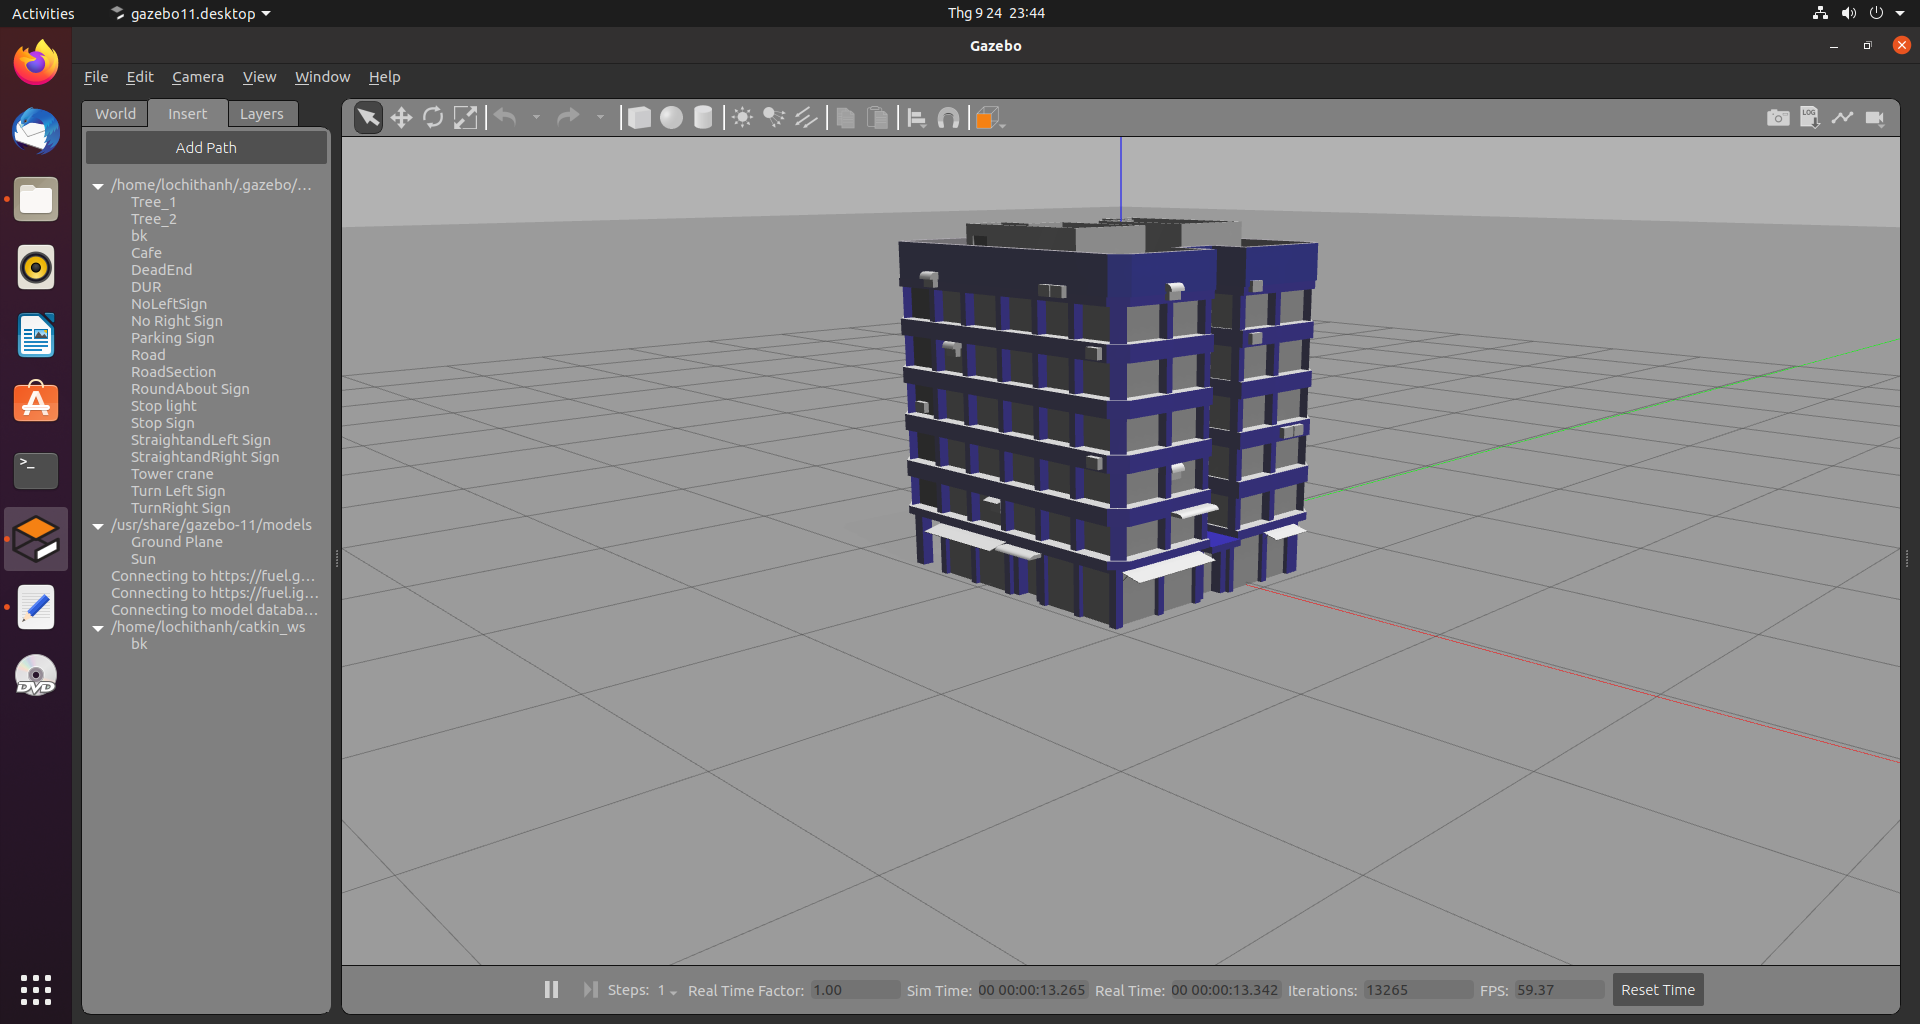
\includegraphics[width=\textwidth]{images/H1.png}
  \caption{Mô hình tòa H3.}

\end{figure}


\begin{figure}[ht]
  \centering
  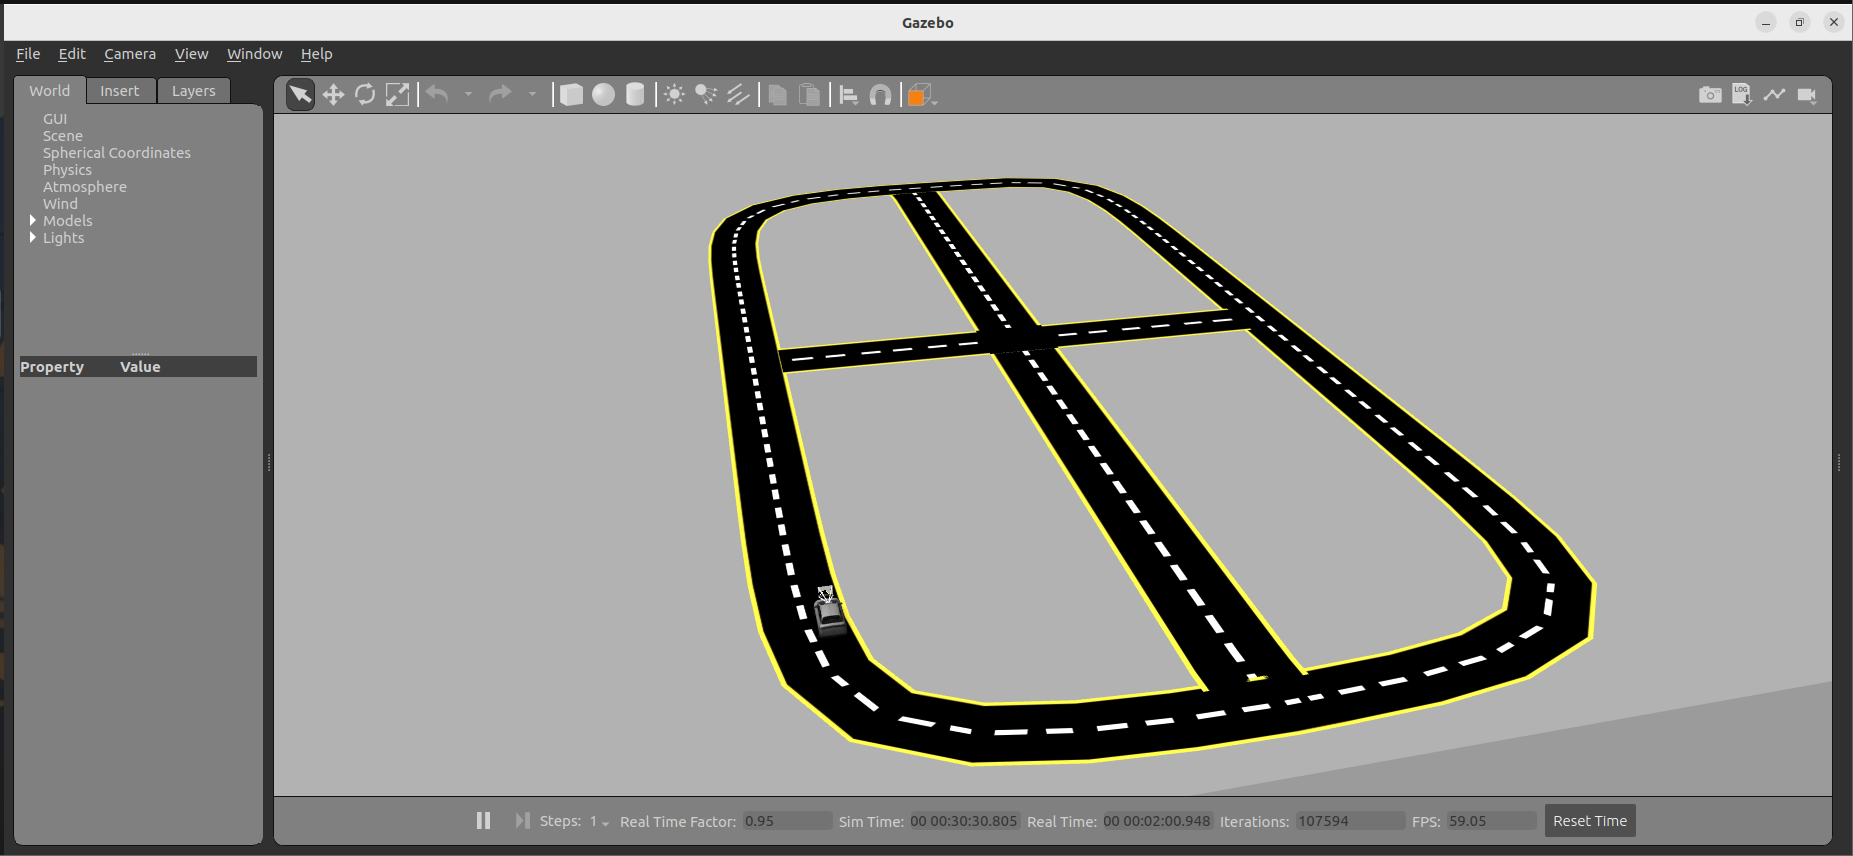
\includegraphics[width=\textwidth]{images/road.png}
  \caption{Test road.}

\end{figure}




















\section{Các khái niệm cần biết}
\subsection{Xử lý ảnh}
\subsubsection{Giới thiệu chung}
Xử lý ảnh là quá trình sử dụng máy tính để thu thập và phân tích các hình ảnh nhằm mục đích trích xuất, cải thiện hoặc biến đổi thông tin hình ảnh. Cụ thể, xử lý ảnh bao gồm các bước: thu thập ảnh, tiền xử lý (c ải thiện chất lượng), phân tích và nhận dạng (phân đoạn ảnh, chiết xuất đặc trưng), ra quyết định/dự đoán dựa trên kết quả phân tích.\\
\newline
Mục đích chính của xử lý ảnh là nâng cao chất lượng hình ảnh, nhận dạng các đối tượng (vật thể, khuôn mặt, chữ viết, v.v.) trong ảnh và hỗ trợ ra quyết định trong các hệ thống thông minh. Xử lý ảnh được ứng dụng rộng rãi trong y tế (phân tích Xquang, CT scanner), bảo mật (nhận dạng khuôn mặt), giao thông (nhận dạng biển báo, xe cộ), nông nghiệp (đánh giá chất lượng nông sản), v.v.
\subsubsection{Tensor trong xử lý ảnh}
Tensor là một khái niệm toán học dùng để biểu diễn dữ liệu đa chiều trong xử lý ảnh và thị giác máy tính.
\begin{itemize}
\item Vector 1D (tensor 1 chiều)
\item Ma trận 2D (tensor 2 chiều)
\item Tensor RGB 3D - [Chiều ảnh, Chiều cao, 3 kênh màu]
\end{itemize}
\newline
So với vector và ma trận thông thường, tensor có thể lưu trữ dữ liệu ở nhiều chiều, thể hiện cấu trúc dữ liệu phức tạp hơn.
Ví dụ:
%
%
%
%
\subsubsection{Convolution trong xử lý ảnh}
Convolution là một phép toán được sử dụng rộng rãi trong xử lý ảnh để tăng cường các đặc trưng mong muốn của ảnh.
\myparagraph{Định nghĩa Convolution}
Convolution là phép nhân 2 hàm f và g để tạo ra hàm mới h:

$h(t) = (f * g)(t) = \int_{-\infty}^{+\infty} f(\tau) g(t - \tau) d\tau$
\newline
Trong đó, $f$ là ảnh input, $g$ là bộ lọc (kernel) và $h$ là ảnh output.
Với mỗi phần tử xij trong ma trận X lấy ra một ma trận có kích thước bằng kích thước của kernel W có phần tử xij làm trung tâm (đây là vì sao kích thước của kernel thường lẻ) gọi là ma trận A. Sau đó tính tổng các phần tử của phép tính \textit{element-wise} của ma trận A và ma trận W, rồi viết vào ma trận kết quả Y.
\begin{equation}
    X=\begin{bmatrix}
        1 & 1 & 1 & 0 & 0 \\
        0 & \colorbox{yellow}{$1$} & 1 & 1 & 0 \\
        0 &  0 & 1 & 1 & 1\\
        0 & 0 & 1 & 1 & 0 \\
        0 & 1 & 1 & 0 & 0
    \end{bmatrix}
    \cdot
    W=\begin{bmatrix}
        1 & 0 & 1 \\
        0 & 1 & 0 \\
        1 & 0 & 1 
       
    \end{bmatrix}
    =
    Y=\begin{bmatrix}
        y_{11} & y_{12}& y_{13} \\
        y_{21} & y_{22}& y_{23} \\
        y_{31} & y_{32}& y_{33}\\
    \end{bmatrix}
\end{equation}
Ví dụ khi tính tại $x_{22}$, ma trận A cùng kích thước với W. Sau đó tính\[
y_{11} = x_{11} \cdot w_{11} + x_{12} \cdot w_{12} + x_{13} \cdot w_{13} + x_{21} \cdot w_{21} + x_{22} \cdot w_{22} + x_{23} \cdot w_{23} + x_{31} \cdot w_{31} + x_{32} \cdot w_{32} + x_{33} \cdot w_{33} = 4
\]

\myparagraph{Convolution trong xử lý ảnh}
Trong xử lý ảnh, convolution được dùng để:

\begin{itemize}
\item Làm nổi bật cạnh của các vật thể
\item Phát hiện các đặc trưng như cạnh, góc, đường thẳng, v.v.
\item Nhận dạng vật thể, khuôn mặt, chữ số, v.v.
\end{itemize}

\subsection{Padding và stride trong Convolution}
Khi thực hiện phép toán convolution trên ảnh, ta cần chú ý 2 thông số là padding và stride.
\subsubsection{Padding}
Padding là việc bổ sung các đường biên 0 xung quanh ảnh input ban đầu. Padding giúp giữ nguyên kích thước ảnh sau khi convolution.\\

Như ở trên thì mỗi lần thực hiện phép tính convolution xong thì kích thước ma trận Y đều nhỏ hơn X. Tuy nhiên giờ ta muốn ma trận Y thu được có kích thước bằng ma trận X => Tìm cách giải quyết cho các phần tử ở viền => Thêm giá trị 0 ở viền ngoài ma trận X.\\
\begin{equation}
X= \begin{bmatrix}
    0 & 0 & 0 & 0 & 0 & 0 & 0 \\
    0 & 1 & 1 & 1 & 0 & 0 & 0 \\
    0 & 0 & 1 & 1 & 1 & 0 & 0 \\
    0 & 0 & 0 & 1 & 1 & 1 & 0 \\
    0 & 0 & 0 & 1 & 1 & 0 & 0 \\
    0 & 0 & 1 & 1 & 0 & 0 & 0 \\
    0 & 0 & 0 & 0 & 0 & 0 & 0 \\
\end{bmatrix}
\end{equation}
\\
Rõ ràng là giờ đã giải quyết được vấn đề tìm A cho phần tử \(x_{11}\) , và ma trận Y thu được sẽ bằng kích thước ma trận X ban đầu.

Phép tính này gọi là convolution với \textbf{padding}=1. Padding=k nghĩa là thêm k vector 0 vào mỗi phía của ma trận.

Các kiểu padding thường dùng:

\begin{itemize}
\item Valid padding: Không thêm pixel biên .
\item Same padding: Thêm đủ số pixel biên để giữ nguyên kích thước.
\item Full padding: Thêm pixel cho tới khi kích thước input bằng nhau.
\end{itemize}
\subsubsection{Stride}
Stride là khoảng cách dịch chuyển của convolution kernel giữa các vị trí trên ảnh input.

Giá trị stride càng lớn thì kích thước ảnh output càng nhỏ.

Giá trị stride thường dùng là 1, 2 hoặc lớn hơn.


Như ở trên ta thực hiện tuần tự các phần tử trong ma trận X, thu được ma trận Y cùng kích thước ma trận X, ta gọi là \textbf{stride}=1.
\begin{equation}
X= \begin{bmatrix}
    0 & 0 & 0 & 0 & 0 & 0 & 0 \\
    0 & 1 & 1 & 1 & 0 & 0 & 0 \\
    0 & 0 & 1 & 1 & 1 & 0 & 0 \\
    0 & 0 & 0 & 1 & 1 & 1 & 0 \\
    0 & 0 & 0 & 1 & 1 & 0 & 0 \\
    0 & 0 & 1 & 1 & 0 & 0 & 0 \\
    0 & 0 & 0 & 0 & 0 & 0 & 0 \\
\end{bmatrix}{stride =1 , padding=1}
\end{equation}

Tuy nhiên nếu stride=k (k > 1) thì ta chỉ thực hiện phép tính convolution trên các phần tử \(x_{1+i \cdot k , 1+j \cdot k}\)

\begin{equation}
X= \begin{bmatrix}
    0 & 0 & 0 & 0 & 0 & 0 & 0 \\
    0 & \colorbox{yellow}{$1$} & 1 & \colorbox{yellow}{$1$} & 0 & \colorbox{yellow}{$0$} & 0 \\
    0 & 0 & 1 & 1 & 1 & 0 & 0 \\
    0 & \colorbox{yellow}{$0$} & 0 & \colorbox{yellow}{$1$} & 1 & \colorbox{yellow}{$1$} & 0 \\
    0 & 0 & 0 & 1 & 1 & 0 & 0 \\
    0 & \colorbox{yellow}{$0$} & 1 & \colorbox{yellow}{$1$} & 0 & \colorbox{yellow}{$0$} & 0 \\
    0 & 0 & 0 & 0 & 0 & 0 & 0 \\
\end{bmatrix}{stride =1 , padding=2}
\end{equation}

Hiểu đơn giản là bắt đầu từ vị trí \(x_{11}\) sau đó nhảy k bước theo chiều dọc và ngang cho đến hết ma trận X.
Công thức tổng quát cho phép tính convolution của ma trận X kích thước m*n với kernel kích thước k*k, stride = s, padding = p ra ma trận Y kích thước \(
(\frac{{m-k+2p}}{{s}}+1) \cdot (\frac{{n-k+2p}}{{s}}+1)\)\\
\textbf{Stride thường dùng để giảm kích thước của ma trận sau phép tính convolution.}
\subsubsection{Ý nghĩa của phép tính convolution }
Mục đích của phép tính convolution trên ảnh là làm mở, làm nét ảnh; xác định các đường;… Mỗi kernel khác nhau thì sẽ phép tính convolution sẽ có ý nghĩa khác nhau. Ví dụ:
\newpage
\begin{figure}[htbp]
        \centering
        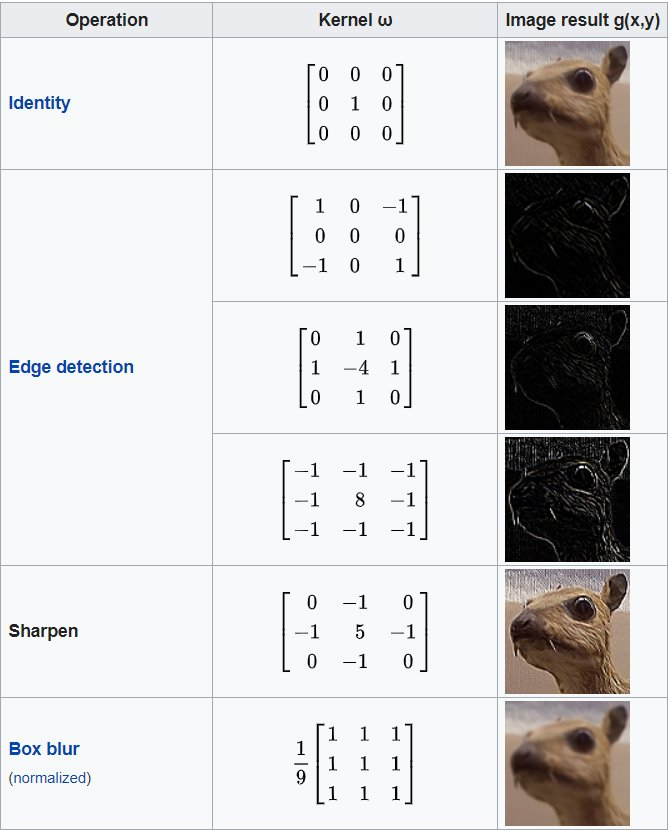
\includegraphics[width=0.6\textwidth]{images/1/image.png}
        \caption{}
\end{figure}
%
%
%
%
%
%
%
%
%
\subsection{Convolutional neutral network}
Mạng CNN là một tập hợp của các lớp Convolution được xếp chồng lên nhau. CNN sử dụng các hàm kích hoạt phi tuyến (như ReLU và tanh) để tạo ra thông tin trừu tượng. Sau khi đi qua các lớp này, mạng thu được trọng số trong các node và tạo ra thông tin trừu tượng cho các lớp kế tiếp.

\noindent Đặc điểm quan trọng của mô hình CNN là tính bất biến và tính kết hợp. Điều này có ảnh hưởng đến độ chính xác của mô hình khi đối tượng được chiếu từ nhiều góc độ khác nhau. \textbf{Pooling layer được sử dụng để tạo tính bất biến đối với các biến đổi như dịch chuyển, co giãn và quay}.

\noindent Các layer convolution giúp thể hiện các cấp độ biểu diễn từ mức độ thấp đến cao, kết hợp thông tin từ các filter. Liên kết giữa các layer đảm bảo kết nối cục bộ hiệu quả nhất. Mỗi nơ-ron trong lớp tiếp theo được tạo ra từ kết quả của convolution thuộc layer trước đó.

\noindent\textbf{ Pooling/subsampling layer được sử dụng để chọn lọc thông tin quan trọng và loại bỏ nhiễu}.
\begin{figure}[htbp]
        \centering
        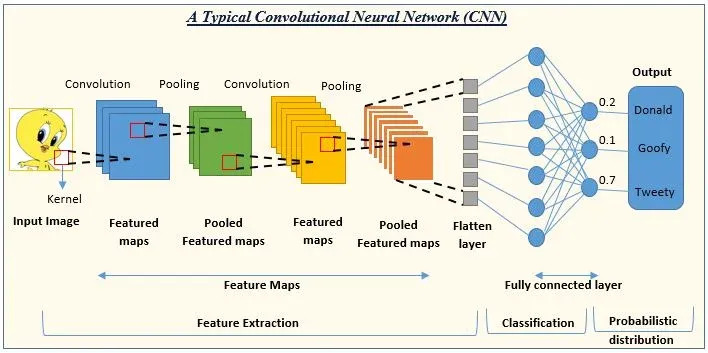
\includegraphics[width=0.6\textwidth]{images/2a-sign/cnn.jpg}
        \newline
        \caption{Cấu trúc của mạng CNN}
\end{figure}
\textbf{Cấu trúc cơ bản nhất của 1 CNN gồm 3 phần là:}
\begin{itemize}
    \item \textbf{Local receptive field (trường cục bộ):}Nhiệm vụ của trường cục bộ là phân tách và lọc dữ liệu cũng như thông tin ảnh, sau đó chọn ra các vùng ảnh có giá trị sử dụng cao nhất. 
    \item \textbf{Shared weights and bias (trọng số chia sẻ):}Trong mạng CNN, thành phần này có tác dụng giảm thiểu tối đa lượng tham số có tác dụng lớn. Trong mỗi convolution sẽ chứa nhiều feature map khác nhau, mỗi feature lại có khả năng giúp nhận diện một số feature trong ảnh. 
    \item \textbf{Pooling layer (lớp tổng hợp):}Pooling layer là lớp cuối cùng, với khả năng đơn giản hóa thông tin đầu ra. Khi đã hoàn tất tính toán và quét qua các lớp, pooling layer sẽ được tạo ra nhằm mục đích lược bớt các thông tin không cần thiết và tối ưu đầu ra. Điều này giúp người dùng nhận được kết quả ưng ý và đúng với yêu cầu hay mong muốn.
\end{itemize}
\begin{figure}[htbp]
        \centering
        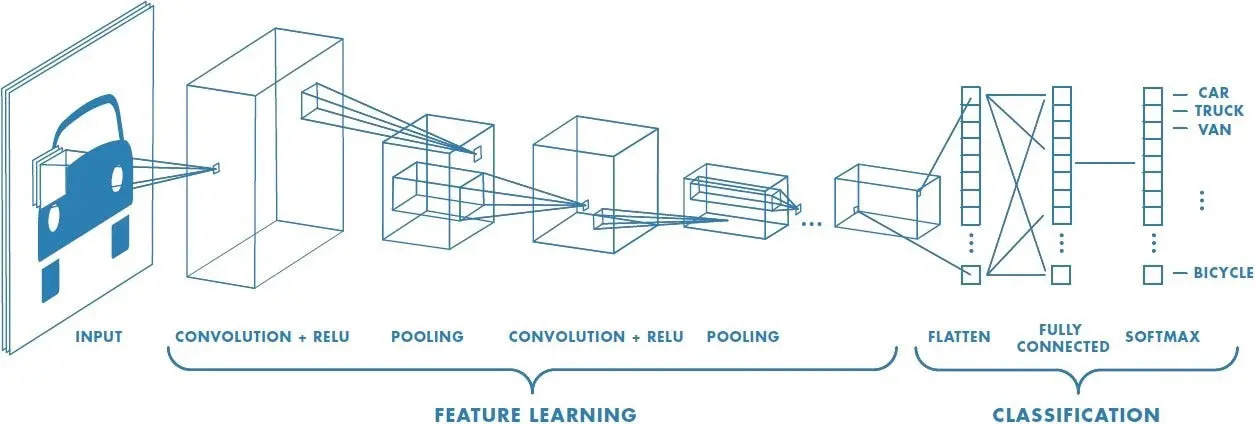
\includegraphics[width=0.7\textwidth]{images/2a-sign/cnn1.jpg}
        
\end{figure}


\section{Nhận diện biển báo giao thông}
Hệ thống nhận diện thường liên quan đến hai nhiệm vụ chính: phát hiện, bao gồm:
\begin{enumerate}
    \item \textbf{Detection: }xác định vị trí và kích thước của đối tượng trong ảnh đầu vào
    \item \textbf{Classification: } gán các đối tượng đã phát hiện vào các lớp con cụ thể
\end{enumerate}
Nhóm đã quyết định tích hợp một mô hình học máy vào hệ thống để cung cấp hỗ trợ trong quá trình nhận diện và phân loại. Để huấn luyện mô hình này, ta cần sử dụng dữ liệu có nhãn. Thay vì phải tự thu thập và gán nhãn, nhóm đã chọn và tận dụng hai bộ dữ liệu có sẵn là GTSDB (German Traffic Sign Detection Benchmark) và GTSRB (German Traffic Sign Recognition Benchmark).


\subsection{Giai đoạn 1: Xác định vị trí biển báo}
\subsubsection{Một số khái niệm}

\subsubsection{Giới thiệu YOLO}
YOLO chia một bức ảnh đầu vào thành một ô lưới có kích thước S×S. Giá trị S được chọn bằng 7 trong paper. Nếu tâm của một vật thể rơi vào một ô nào thì ô đó sẽ chịu trách nhiệm cho việc tìm kiếm vật thể đó.

\begin{figure}[htp]
  \centering
  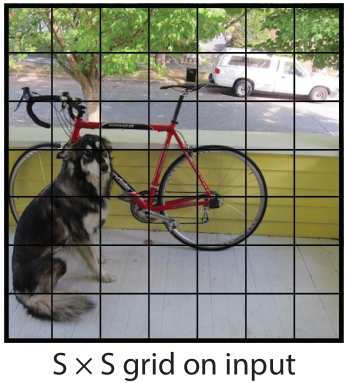
\includegraphics[width=0.4\textwidth]{images/2a-sign/grid1.png}
  \caption{Lưới 7x7}
\end{figure}

\noindent Hình trên là một ví dụ về một bức ảnh đầu vào được chia thành một ô lưới có kích thước S×S. Trong YOLO, giá trị S được chọn bằng 7. 
Mỗi grid cell sẽ dự đoán B bounding boxes và confidence score cho mỗi box đó. Ta sẽ xét kỹ hơn hai khái niệm này ngay dưới đây.\\

\noindent Confidence score sẽ phản ánh hai thông số:
\begin{itemize}
    \item Mức độ tự tin của mô hình trong việc dự đoán box đó chứa vật thể.
    \item Độ chính xác của predicted box là bao nhiêu (tức box đó khớp với ground-truth box đến mức nào).
\end{itemize}
Từ hai ý trên, ta định nghĩa confidence score một cách chặt chẽ hơn như sau: $Pr(Object)$ x $IOU^{truth}_{pred}$.\\
Từ công thức trên, ta có thể rút ra một vài nhận xét như sau:
\begin{itemize}
    \item Nếu không có vật thể nào tồn tại trong cell đó thì  p(Object) = 0 $\Rightarrow$ confidence score = 0.
    \item Ngược lại, nếu cell đó chứa vật thể $\Rightarrow$ p(Object) = 1, , vì thế ta kỳ vọng confidence score = IOU giữa predicted box và ground truth box.
\end{itemize}
Mỗi bounding box thể hiện 5 giá trị x, y, w, h, confidence:
\begin{itemize}
    \item (x, y) là tọa độ tâm (offset) của bounding box so với với vị trí của của grid cell, vì thế nên giá trị của x, y sẽ rơi vào đoạn [0,1].
    \item w, h là width, height của bounding boxes, được chuẩn hóa theo width và height của bức ảnh gốc, vì thế giá trị của chúng sẽ rơi vào đoạn [0,1].
    \item Confidence biểu diễn giá trị IOU giữa predicted box và ground truth box.
    \begin{figure}[htbp]
        \centering
        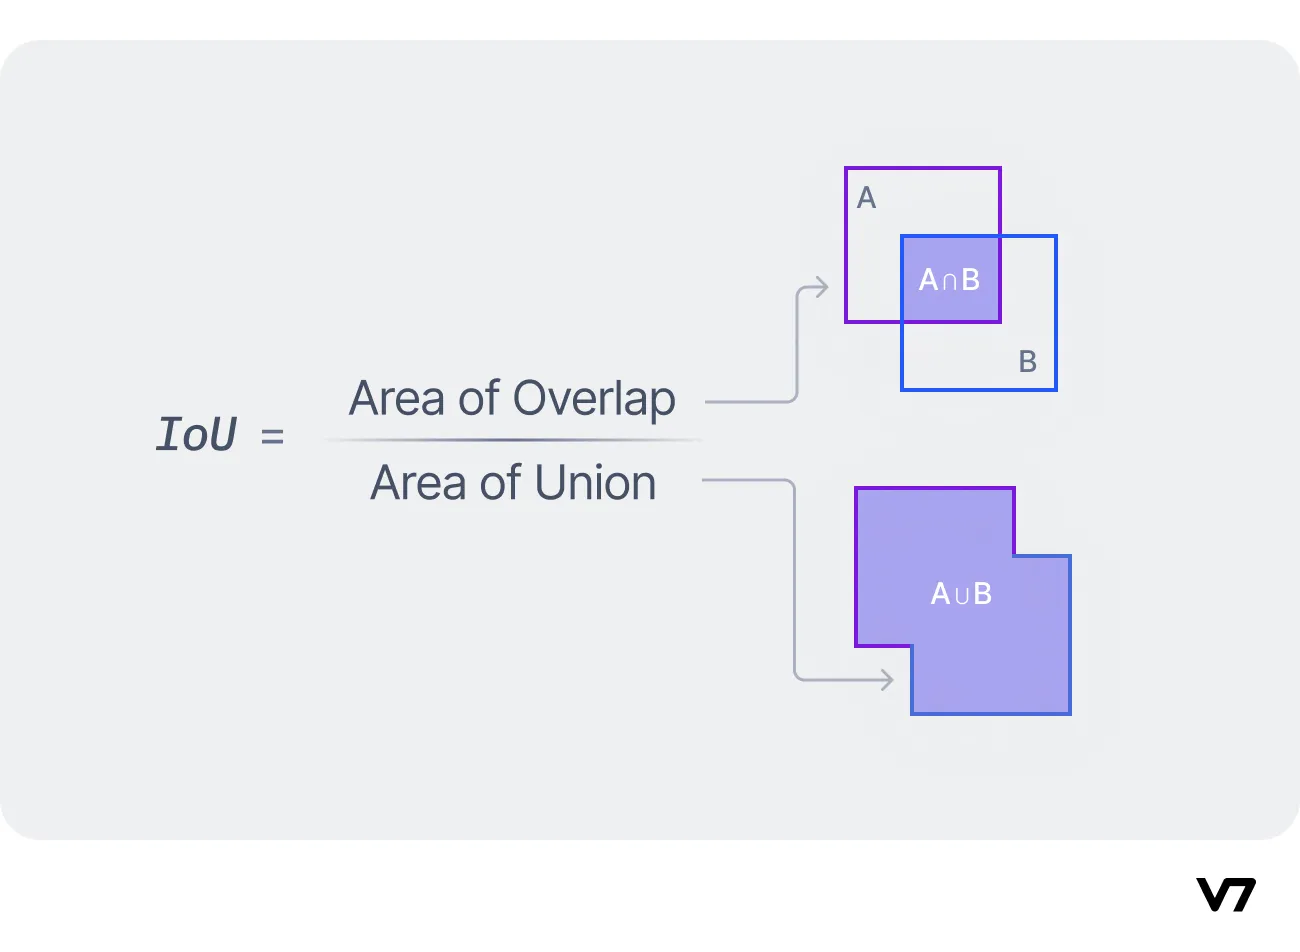
\includegraphics[width=0.6\textwidth]{images/2a-sign/IOU.png}
        \caption{Intersection over Union}
    \end{figure}
\end{itemize}
Mỗi grid cell cũng sẽ dự đoán C xác suất có điều kiện của các class: $p(Class_{i}|Object)$ (Các xác suất này được lấy điều kiện trên grid cell chứa đối tượng).

\noindent Tại thời điểm test, ta nhân xác suất có điều kiện của mỗi class với dự đoán confidence của từng box như sau: 
\begin{center}
    $p(Class_{i}|Object)$ x $p(Object$ x $IOU^{truth}_{pred}$ = $p(Class_{i})$ x $IOU^{truth}_{pred}$
\end{center}
Công thức trên cho ta confidence scores của từng class cho mỗi box. Công thức này cho ta biết:
\begin{itemize}
    \item Xác suất của $class_i$ xuất hiện trong box đó
    \item Độ khớp của của predicted box so với vật thể.
\end{itemize}
Như vậy, có thể tóm gọn lại quy trình hoạt động của YOLO như sau:
\begin{figure}[htbp]
        \centering
        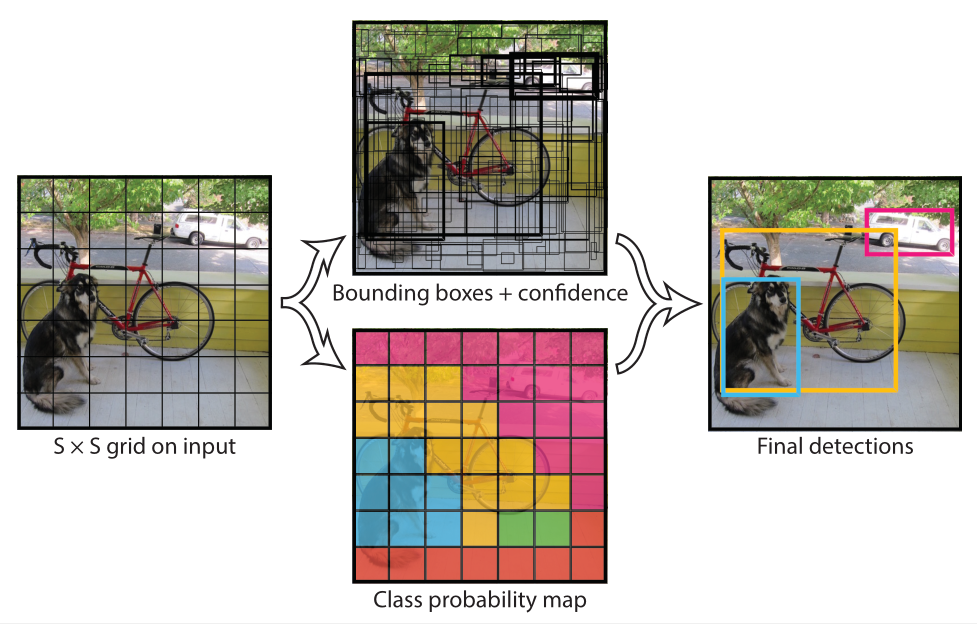
\includegraphics[width=0.6\textwidth]{images/2a-sign/grid2.png}
        \caption{Quy trình của YOLO}
\end{figure}
Trong phạm vi của đề tài này, quyết định của nhóm là sử dụng mô hình YOLOv3 để thực hiện nhiệm vụ nhận diện và định vị đối tượng. Để hiểu rõ hơn về lựa chọn này, nhóm sẽ giới thiệu không chỉ về YOLOv3 mà còn về các phiên bản trước đó bao gồm YOLOv1 và YOLOv2. Điều này giúp ta có cái nhìn tổng quan về sự tiến triển và cải tiến của mô hình YOLO theo thời gian, cũng như lý do mà YOLOv3 được chọn làm nền tảng cho nghiên cứu và thực nghiệm của nhóm.

\subsubsection{YOLOv1}
\myparagraph{Kiến trúc}
Kiến trúc mạng YOLOv1 được lấy ý tưởng từ mô hình GoogLeNet cho phân loại ảnh. Nó gồm có 24 Convolutional Layers dùng để trích xuất các features từ bức ảnh, theo sau bởi 2 Fully Connected Layers để dự đoán output probabilities và coordinates. Thay vì sử dụng inception modules trong GoogLeNet, YOLO chỉ sử dụng reduction layers có kích thước 1x1 theo sau bởi Convolutional Layers có kích thước 3x3 
\begin{figure}[htbp]
        \centering
        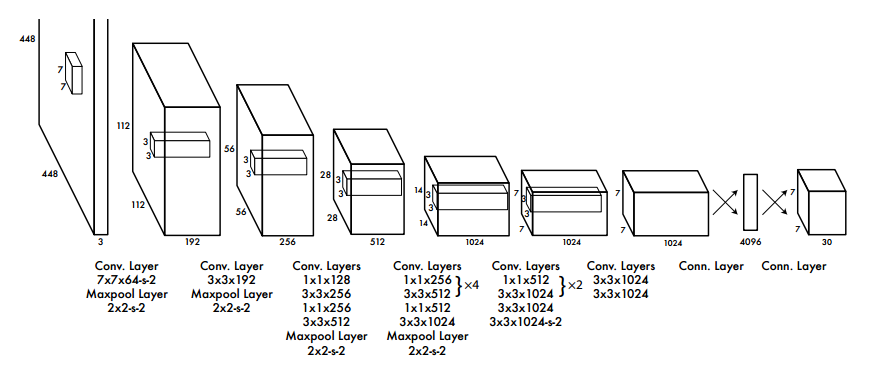
\includegraphics[width=0.8\textwidth]{images/2a-sign/yolo1_arch.png}
        \caption{Kiến trúc YOLOv1}
\end{figure}

\myparagraph{Hàm mất mát}
\begin{figure}[htbp]
        \centering
        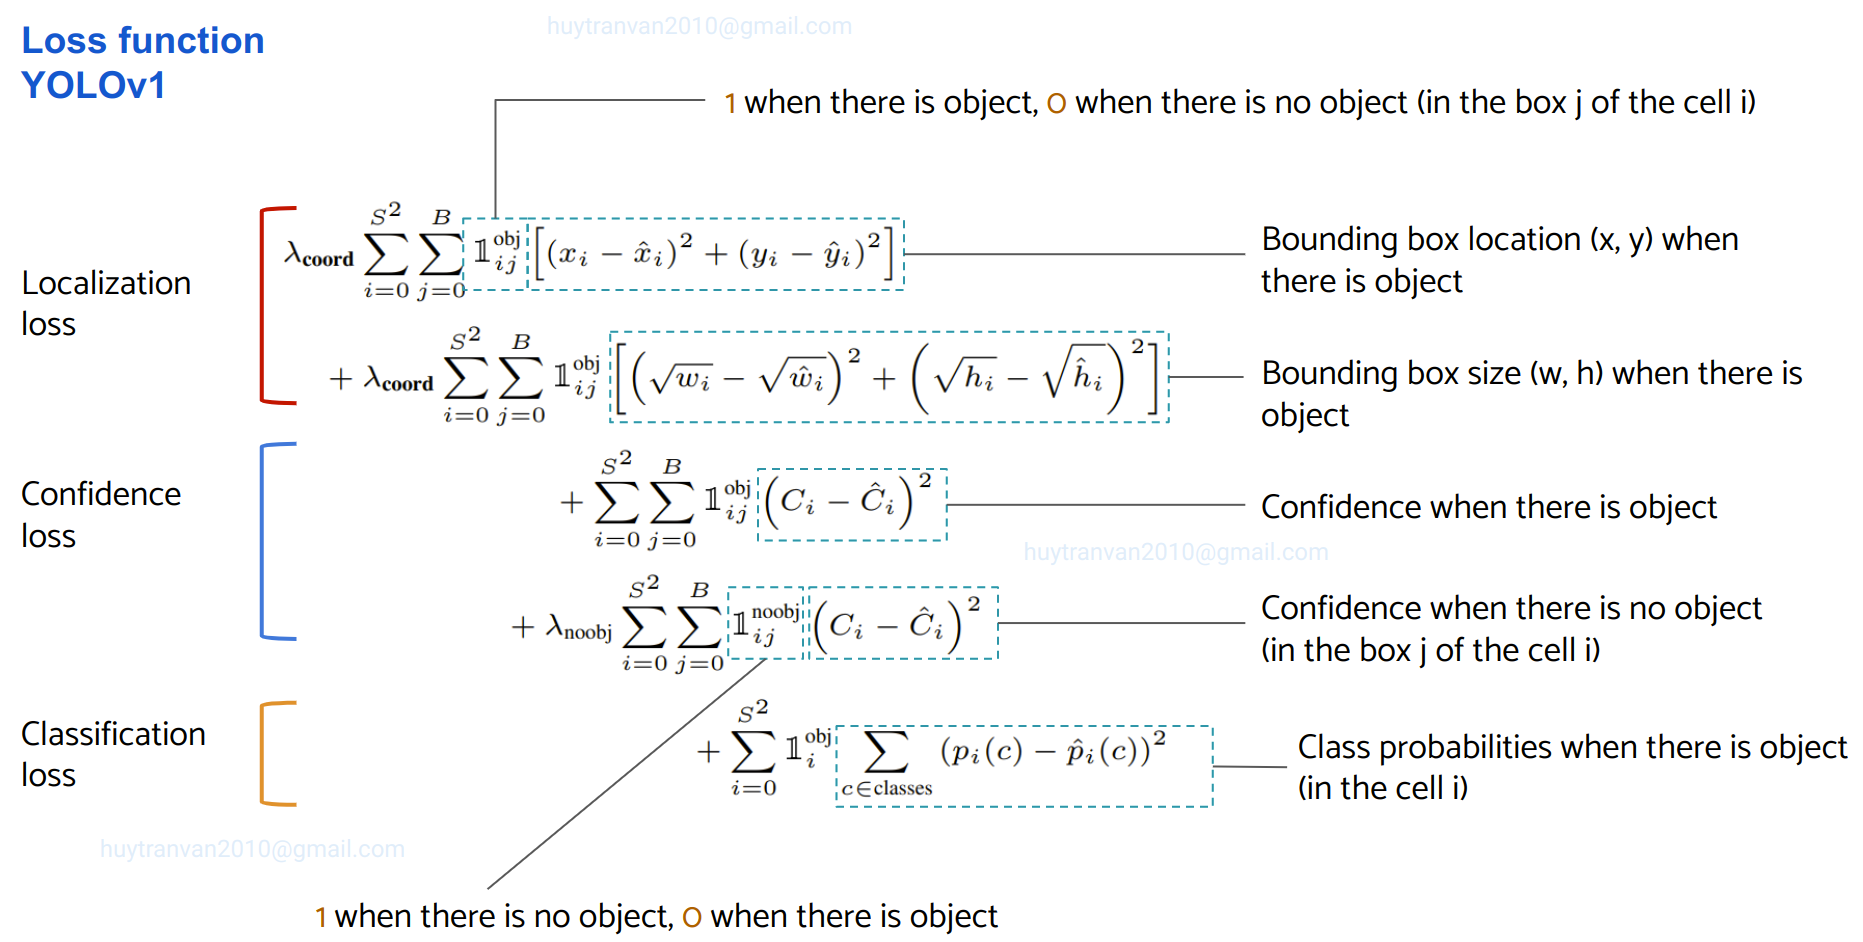
\includegraphics[width=0.8\textwidth]{images/2a-sign/YOLO_loss.png}
        \caption{Hàm mất mát tổng quát}
\end{figure}
\begin{itemize}
    \item \textbf{Localization loss}
    \begin{equation*}
\mathcal{L}_{loc} = \lambda_{coord} \sum_{i=0}^{S^2} \sum_{j=0}^B \mathds{1}_{ij}^{obj} [(x_i - \hat{x}_i)^2 + (y_i - \hat{y}_i)^2 ] +\lambda_{coord} \sum_{i=0}^{S^2} \sum_{j=0}^B \mathds{1}_{ij}^{obj} [(\sqrt{w_i} - \sqrt{\hat{w}_i})^2 + (\sqrt{h_i} - \sqrt{\hat{h}_i})^2]
    \end{equation*}
$\mathds{1}_{i}^{obj}$ = 1 thể hiện trong cell i có object xuất hiện (ngược lại thì bằng 0).\\
$\mathds{1}_{i}^{obj} = 1$ nếu box j của grid cell i có chứa object, ngược lại bằng 0. Ở đây grid cell i phải chứa object trước đã, chứa object rồi thì mới khớp được với prediected box.\\

Khi huấn luyện chúng ta đã biết grounth-truth box thuộc cell nào. Khi dự đoán đưa ra nhiều predicted boxes cho mỗi grid cell. Chúng ta chỉ muốn duy nhất một predicted box chịu trách nhiệm cho object của grid cell. Do đó box thứ j được coi chứa object trong grid cell i là predicted box có IoU cao nhất trong 2 boxes thuộc grid cell đó. Trong hoàn cảnh này tất nhiên đang đề cập đến grid cell i
 có object.
\begin{figure}[htbp]
    \centering
    \subfigure[htp]{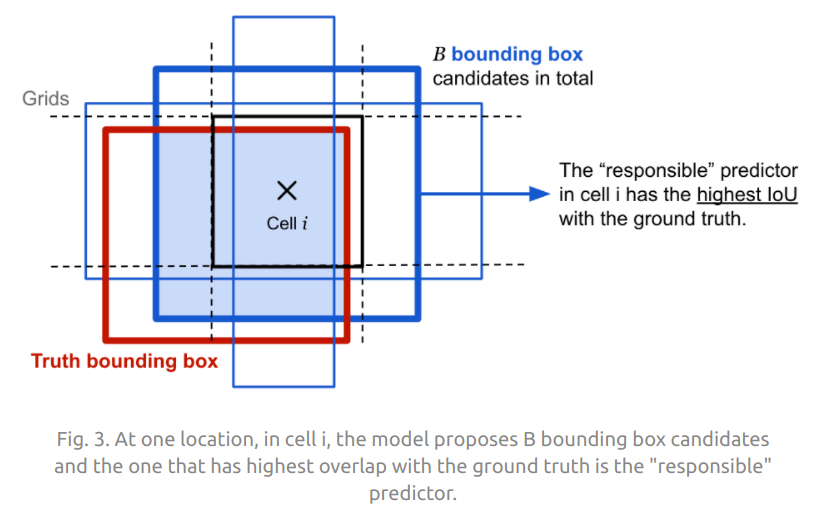
\includegraphics[width=0.4\textwidth]{images/2a-sign/L-loss1.png}}
    \subfigure[htp]{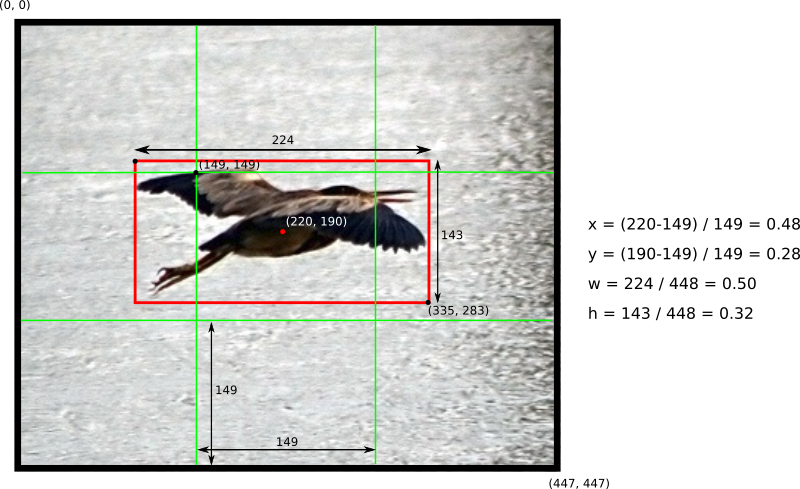
\includegraphics[width=0.4\textwidth]{images/2a-sign/L-loss2.png}}
\end{figure}

Trong loss function $\mathcal{L}_{loc}$ nhận thấy width và height dùng square root (căn bậc 2). Điều này để tính đến việc chênh lệch giữa hai box lớn ít bị ảnh hưởng hơn so với chênh lệch giữa hai box nhỏ. Cùng lấy ví dụ để hiểu rõ hơn. Ví dụ chúng ta lấy $\omega_1 = 0.55$, $\hat{\omega}_1 = 0.5$, $\omega_2 = 0.5$, $\hat{\omega}_2 = 0.45$, nhận thấy $\omega_1 - \hat{\omega}_1 = 0.5 = \omega_2 -\hat{\omega}_2$, tuy nhiên bounding boxes nhỏ hơn $\omega_2 = 0.5$, $\hat{\omega}_2 = 0.45$ bị lệch nhiều hơn so với bounding boxes lớn $\omega_1 = 0.55$, $\hat{\omega}_1 = 0.5$. Vì vậy, lấy căn bậc 2 của giá trị này sẽ làm giảm độ ảnh hưởng của Bounding Box lớn khi có lệch nhỏ. 
    \item \textbf{Confidence loss (hay object loss)}
    \begin{equation*}
        \mathcal{L}_{obj} = {\sum_{i=0}^{S^2} \sum_{j=0}^B \mathds{1}_{ij}^{obj} (C_{ij} - \hat{C}_{ij})^2} +\lambda_{noobj}{\sum_{i=0}^{S^2} \sum_{j=0}^B \mathds{1}_{ij}^{noobj} (C_{ij} - \hat{C}_{ij})^2}
    \end{equation*}
Thành phần thứ nhất của object loss chính là phần loss cho trường hợp cell i có chứa objet, tức là $C_i = 1, C_{ij} = 1,\hat{C}_{ij} = Pr(object) . IOU_{pred}^{truth}$ là giá trị dự đoán cho bounding box j thuộc cell i.\\
Thành phần thứ nhất của object loss chính là phần loss cho trường hợp ngược lại, cell i không chứa objet, tức là $C_i = 0, C_{ij} = 0,\hat{C}_{ij} = Pr(object) . IOU_{pred}^{truth}$ là giá trị dự đoán cho bounding box j thuộc cell i.\\

$\mathds{1}_{ij}^{obj} = 1 (\mathds{1}_{ij}^{noobj} = 0)$ nếu box j của cell i có chứa vật thể, và $\mathds{1}_{ij}^{obj} = 0 (\mathds{1}_{ij}^{noobj} = 1)$ cho trường hợp ngược lại. Ở đây cứ grid cell và box của nó không match với nhau thì cho vào nhóm này, bao gồm cả những grid cell không chứa object và grid cell chứa object nhưng không khớp với box do có IoU nhỏ hơn box còn lại. Và những trường hợp không khớp như này chúng ta chỉ đi minimize objectness score, không quan tâm đến coordinates và class probabilities (vì vốn dĩ đã không chứa object).
\begin{figure}[htbp]
        \centering
        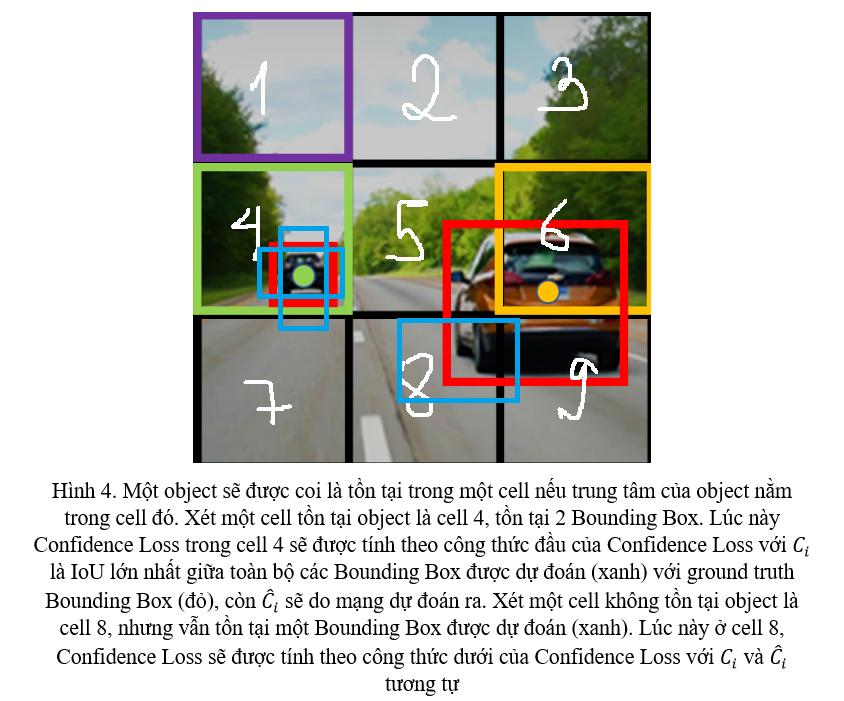
\includegraphics[width=0.5\textwidth]{images/2a-sign/L-loss3.png}
        \caption{Minh họa confidence loss}
\end{figure}

Ở đây, có một điều cần chú ý là trong ảnh đa số các grid cell không chứa object nên nếu để weights của localization loss và confidence loss cho vị trí không có object như nhau thì kết quả sẽ không tốt. Model lúc này có xu hướng tập trung dự đoán các box không chứa object để giảm loss nhiều nhất có thể. Do đó ở đây sẽ thiết lập weights khác nhau $\lambda_\text{noobj} =0.5, \lambda_\text{coord} = 5$ để tăng hiệu suất của model.
    \item \textbf{Classification loss}
\begin{equation*}
    \mathcal{L}_{cls}={\sum_{i=0}^{S^2} \mathds{1}_i^{obj}  \sum_{c \in classes} (p_i(c) - \hat{p}_i(c))^2}
\end{equation*}
trong đó $1^{obj}_{i}=1$ nếu grid cell thứ i chứa object.\\

$p_i(c)=Pr(class_i \mid object)$ được tính chung cho cả grid cell không phụ thuộc vào số bounding boxes của grid cell. Phần loss này chung cho grid cell có chứa object. Nếu class nào xuất hiện trong grid cell đó thì ta có $p(c) = 1$, các classes còn lại bằng 0.
\end{itemize}

\myparagraph{Non-Max Suppression}
Chú ý khi nhận diện có rất nhiều bounding boxes có thể phụ trách cho một vật thể. Để loại bỏ bớt các bounding boxes thừa chúng ta sẽ áp dụng Non-Max Supression. Tuy nhiên trước tiên chúng ta cần biến đổi ouput một chút. Ở bên trên chúng ta cũng đã đề cập:
\[
Pr(class_i | object) \cdot Pr(object) \cdot IOU_{pred}^{truth} = Pr(class_i) \cdot IOU_{pred}^{truth}
\]
Tương ứng với mỗi bounding box chúng ta sẽ có 20 giá trị $Pr(class_i) \cdot IOU_{pred}^{truth}$ thể hiện score của từng class trong bounding box có tính đến sự khớp với ground truth box. Tổng cộng chúng ta có $98 \times 20 = 1960$  các giá trị như này cho 98 bounding boxes do mỗi có $7 \times 7$ grid cell, mỗi cell có 2 boxes. Thực chất việc đưa về tensor $7 \times 7 \times 30 = 1470$ giúp chúng ta giảm số tham số trong mô hình thay vì phải dùng FC layer với 1960 units. Sau FC layer với 1470 units chúng ta reshape lại về tensor $7 \times 7 \times 30$  như hình bên dưới.
\begin{figure}[htbp]
        \centering
        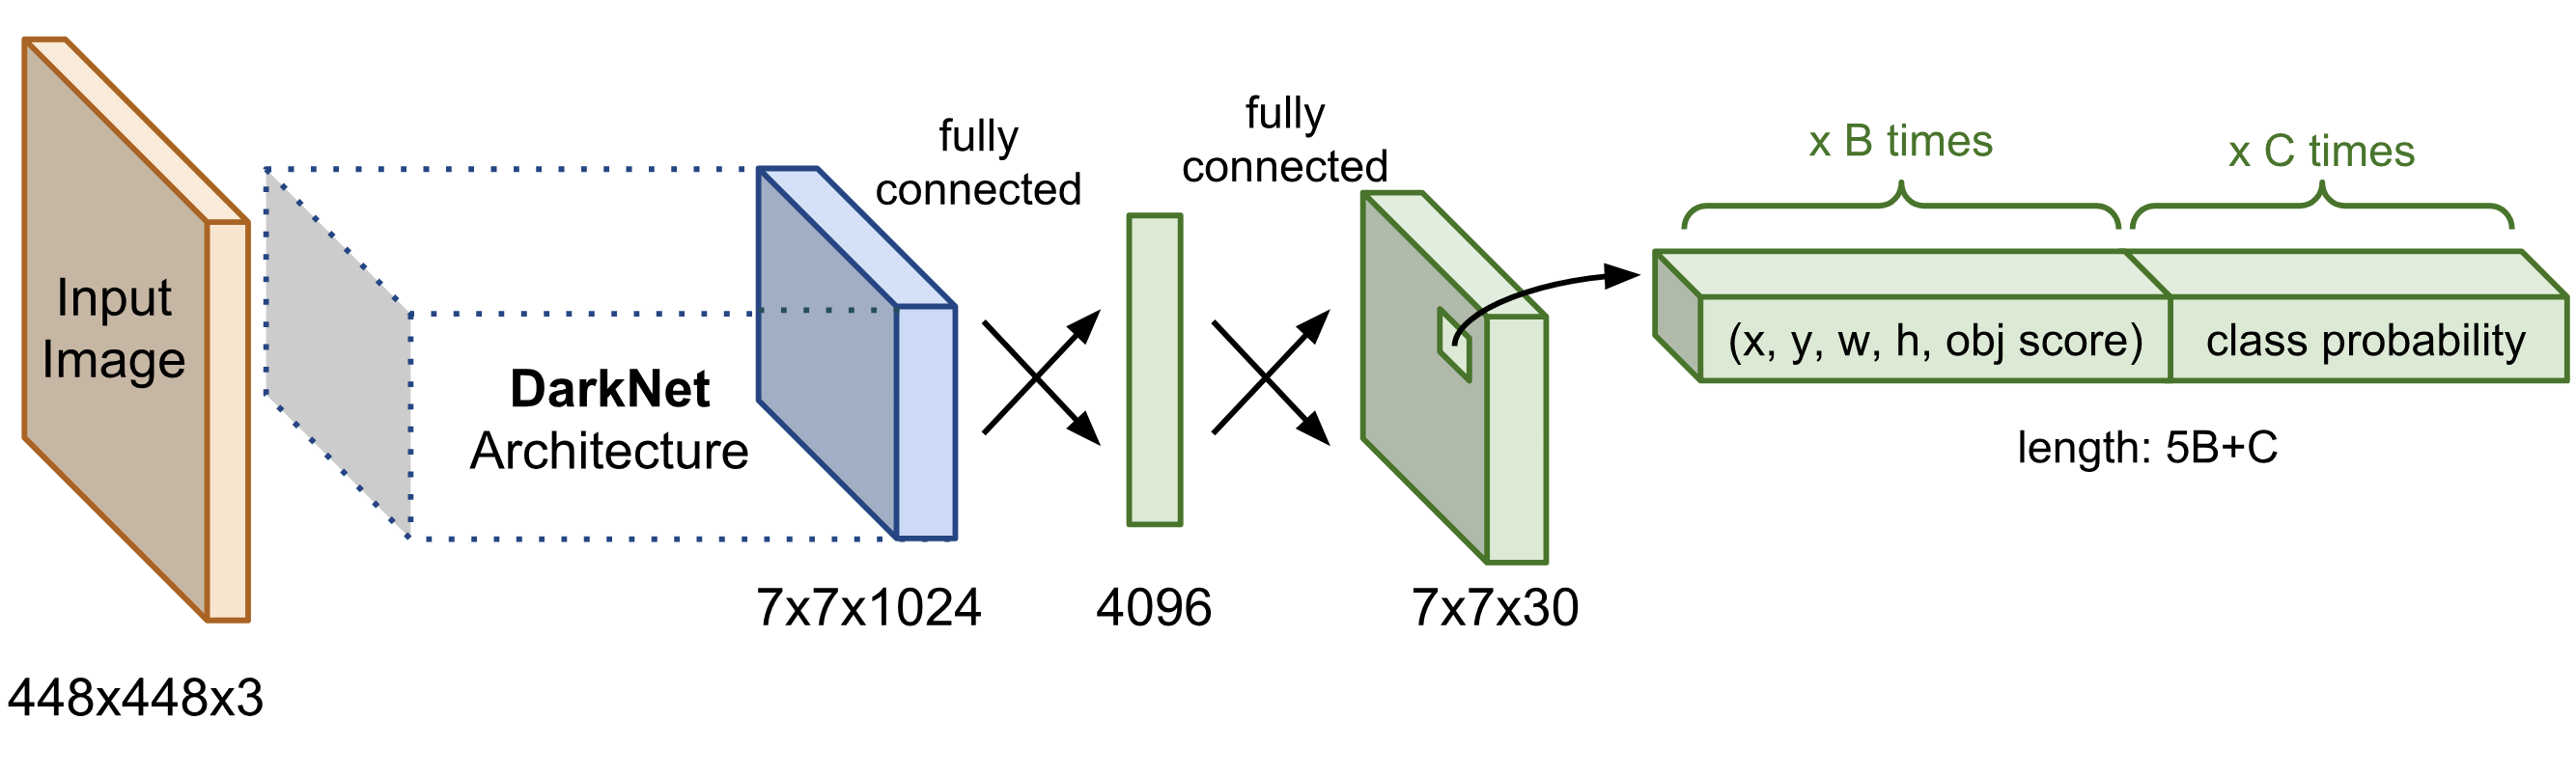
\includegraphics[width=0.6\textwidth]{images/2a-sign/1.png}
\end{figure}

\begin{figure}[htbp]
        \centering
        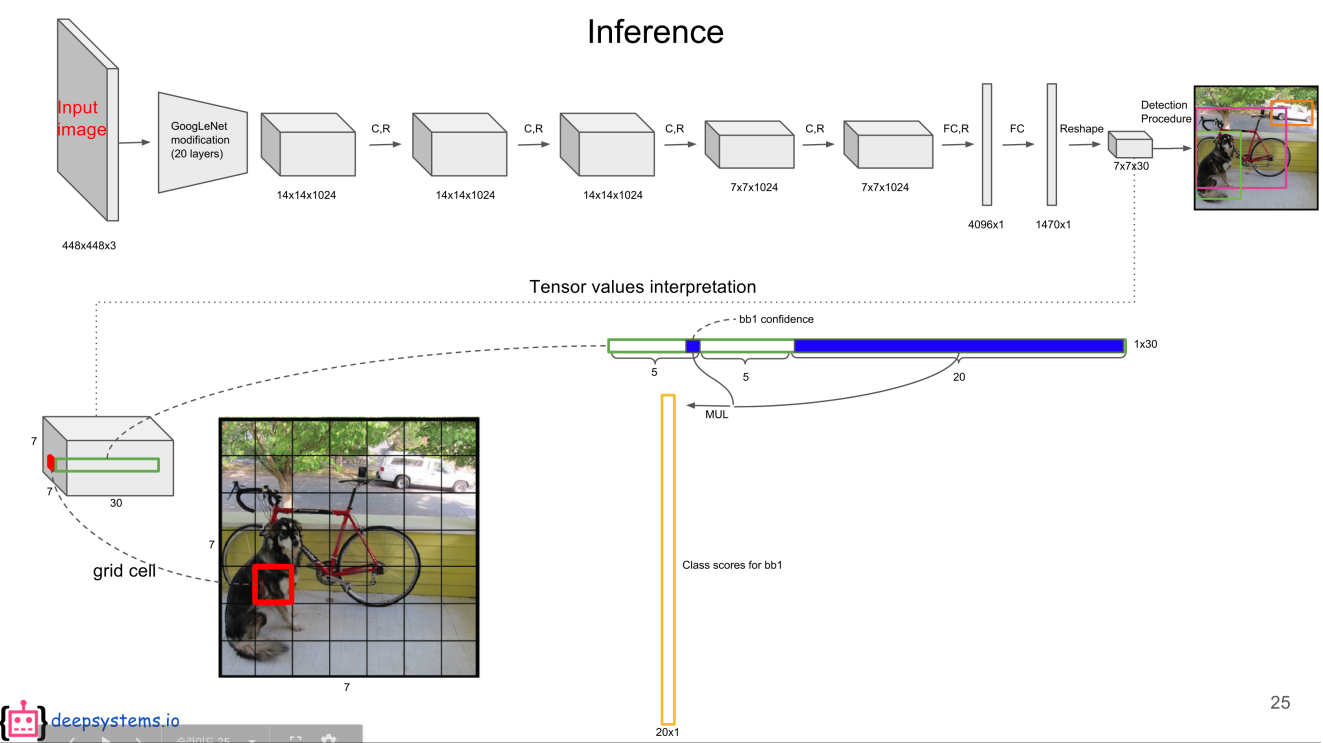
\includegraphics[width=0.6\textwidth]{images/2a-sign/yolo1_inference.png}
\end{figure}
Sau đó chúng ta cần biến đổi một chút để có được class score cho mỗi bounding box như đã trình bày ở phần trên. Chúng ta có tổng cộng 98 predicted bounding boxes. Quá trình NMS có thể được tóm tắt như hình dưới đây:
\newpage
\begin{figure}[h]
        \centering
        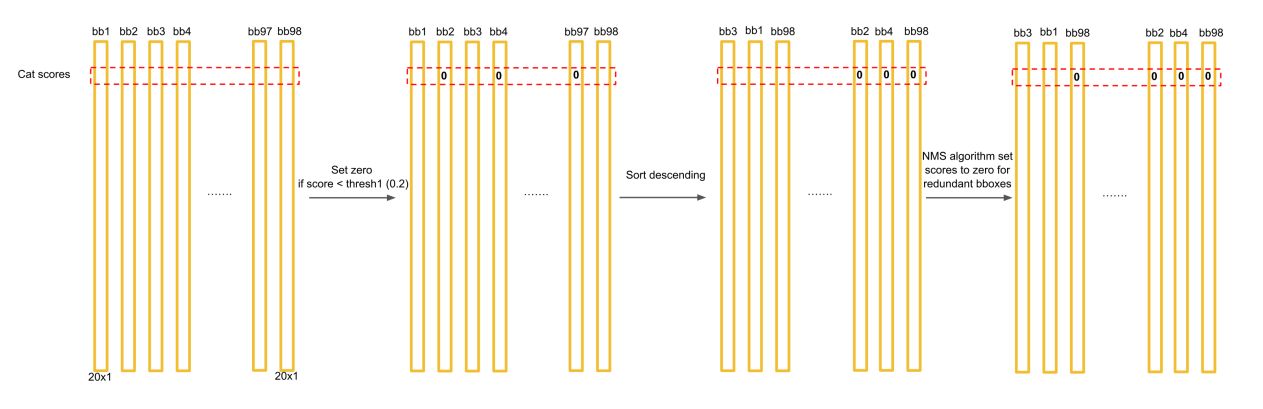
\includegraphics[width=0.8\textwidth]{images/2a-sign/yolo1_nms.png}
\end{figure}

Để đơn giản gọi $Pr(class_i) \cdot IOU_{pred}^{truth}$ là class confidence - kết quả sau khi thực hiện phép nhân. Xét cho tất cả bounding boxes:
\begin{itemize}
    \item Đối với $c_1$ class đầu tiên, nếu class confidence $c_1$ 
 của box nào nhỏ hơn threshold score thì set class confidence của box đó = 0
 \item Sắp xếp boxes theo chiều giảm của class confidence $c_1$
 \item Áp dụng NMS bắt đầu từ box bên trái có class confidence 
 $c_1$ lớn nhất, các box phía bên phải có IOU so với box đầu lớn hơn IOU threshold thì set class confidence của box đó = 0.
 \item Làm xong với box bên trái có class confidence $c_1$
 max rồi sẽ làm tiếp đến box còn lại (có class confidence $c_1$
 còn khác 0)
\item Cứ làm như vậy đến khi bên tay phải không còn box nào có class confidence $c_1$ khác 0. Như vậy xong cho một class. Lúc này class confidence của class đó trong các boxes được chọn sẽ lớn hơn 0, và bằng 0 trong các boxes không được chọn.
\item Lặp lại các bước trên lần lượt cho các class còn lại.
\end{itemize}
Sau khi thực hiện xong các bước trên sẽ đến bước vẽ các bounding box. Nên nhớ sau khi xử lý trong một bounding box có thể có nhiều class confidences khác 0. Đối với mỗi bounding box sẽ chọn ra class có confidence lớn nhất. Giá trị của class confidence này phải lớn hơn 0. Khi đó bounding box là hợp lệ có chứa thông tin class, class confidence và các thông số hình học.
\begin{figure}[htbp]
        \centering
        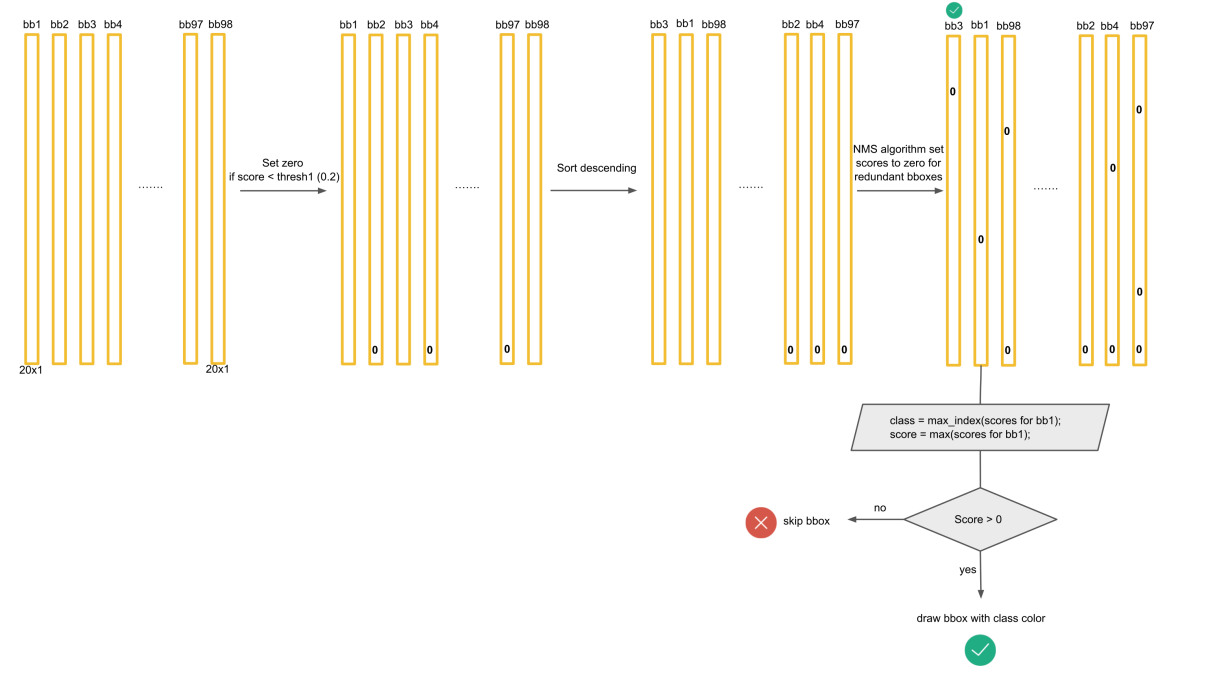
\includegraphics[width=0.8\textwidth]{images/2a-sign/yolo1_nms2.png}
\end{figure}

\subsubsection{YOLOv3}
YOLOv3 có kiến trúc khá giống YOLOv2. Tác giả đã thêm các cải tiến mới trong các nghiên cứu object detection thời điểm đó vào YOLOv2 để tạo ra YOLOv3. Base network mới được dùng, lớn hơn Darknet-19 nhưng vẫn đảm bảo được tốc độ inference.
\myparagraph{Dự đoán bounding box}
Trong dự đoán của mỗi box sẽ có các giá trị $t_x, t_y, t_w, t_h$ và objectness prediction - những giá trị này được sử dụng để tính loss. Nếu grid cell offset so với góc trên bên trái của ảnh $(c_x, c_y)$ và anchor box có width và height $p_w, p_h$ thì predictions (được tính toán lại, không phải output của model) sẽ là
\begin{equation*}
    \begin{aligned}
b_x &= \sigma(t_x) + c_x\\
b_y &= \sigma(t_y) + c_y\\
b_w &= p_w e^{t_w}\\
b_h &= p_h e^{t_h}\\
\end{aligned}
\end{equation*}
\begin{figure}[htp]
    \centering
    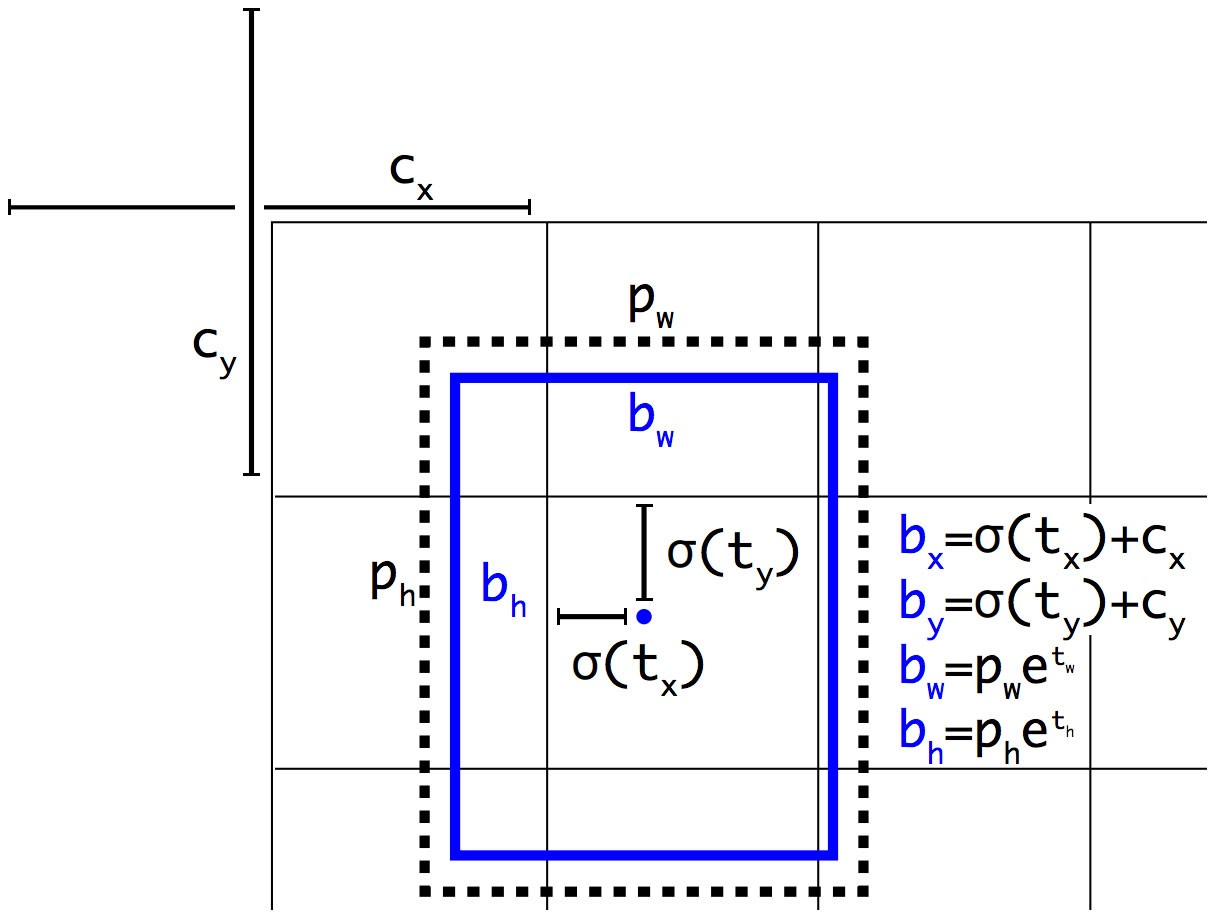
\includegraphics[width=0.4\textwidth]{images/2a-sign/yolov3.jpeg}
    \caption{Bounding box location prediction}
\end{figure}

$(c_x, c_y)$ - tọa độ góc trên bên trái của grid cell chứa anchor box tương ứng. Tọa độ này được xác định sau khi đã chia grid cell, ví dụ như hình bên trên $c_x = 1, c_y = 1$. $p_w, p_h$ cũng vậy,cũng được normalize theo width và height sau khi đã chia grid cell.\\
\newline
YOLOv3 dự đoán objectness score cho mỗi bounding box bằng logistic regression. Nếu bounding box prior (anchor) overlap với ground-truth box lớn hơn so với các anchor boxes khác thì objectness score bằng 1. Nếu anchor box không có IoU lớn nhất nhưng overlap với ground-truth box và IoU lớn hơn threshold 0.5 thì chúng ta bỏ qua dự đoán đó - không tính loss. Mỗi ground-truth box chỉ liên quan đến một anchor box. Nếu anchor box không được gán cho ground-truth box nào thì khi tính loss cho nó sẽ bỏ qua classification loss, localization loss và chỉ tính confidence loss cho object - liên quan đến việc có object hay không.

\myparagraph{Dự đoán các lớp}
Mỗi box dự đoán các classes mà box đó có thể chứa bằng multilabel classification. Chúng ta không sử dụng softmax và thay vào đó sử dụng các logistic classifiers độc lập với nhau. Trong suốt quá trình training thì sử dụng binary cross-entropy loss cho class predictions. Thông thường chỉ sử dụng softmax khi mỗi box có duy nhất một class, tuy nhiên với nhiều dataset các objects có thể rất gần nhau và việc sử dụng này không hiệu quả.

\myparagraph{Trích xuất đặc trưng}
YOLOv3 sử dụng mạng neural network mới để trích xuất đặc trưng Darknet-53. Darknet-53 vẫn dựa trên sự thành công của 3x3, 1x1 Conv layers giống như kiến trúc Darknet-19 cũ, tuy nhiên ở đây sử dụng thêm residual blocks. Model mới có 53 Conv layers nên gọi là DarkNet-53.
\begin{figure}[htp]
    \centering
    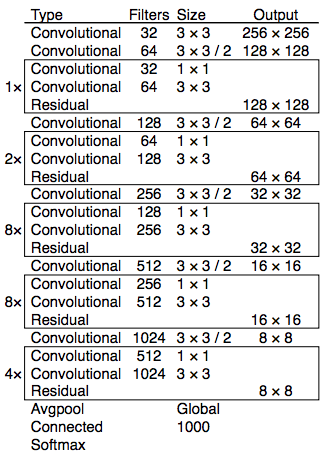
\includegraphics[width=0.4\textwidth]{images/2a-sign/yolov3_archi.png}
    \caption{Kiến trúc Darknet-53}
\end{figure}

\noindent Darknet-53 mạnh mẽ hơn so với Darknet-19. Darknet-53 tốt hơn so với ResNet-101 và nhanh hơn 1.5 lần. Darknet-53 có performnace tương đương ResNet-152 nhưng nhanh hơn 2 lần.\\

\noindent Darknet-53 có BFLOP/s (billion floating point operations per second) lớn. Điều này có nghĩa rằng kiến trúc của Darknet-53 sử dụng tốt GPU, giúp nó có tốc độ nhanh hơn.
\myparagraph{Multi-scale prediction}
YOLOv3 đưa ra dự đoán cho 3 scales khác nhau. YOLOv3 trích xuất features từ những scales này bằng cách sử dụng khái niệm tương tự Feature Pyramid Network. Từ base feature extractor sẽ thêm một số Conv layers.\\
Ở mỗi scale sẽ dự đoán 3 boxes cho mỗi vị trí (grid cell), do đó output tensor cho mỗi scale là N x N x [3 x (4 + 1 + 80)] với:
\begin{itemize}
    \item 4 bounding box offsets
    \item 1 objectness prediction
    \item 80 class predictions
\end{itemize}
Cụ thể việc dự đoán cho 3 scales khác nhau là:
\begin{itemize}
    \item Ở feature map cuối cùng
    \item Feature map ở trước đó 2 layers, feature map được được upsample 2x. YOLOv3 lấy feature map có resolution lớn hơn (ở trước nữa trong mạng NN) và kết hợp với upsampled feature thông qua concatenation. Sau đó áp dụng một số Conv layers và dự đoán output cuối cùng.
    \item Thực hiện thiết kế như scale thứ 2 cho scale thứ 3.
\end{itemize}

\begin{figure}[htp]
    \centering
    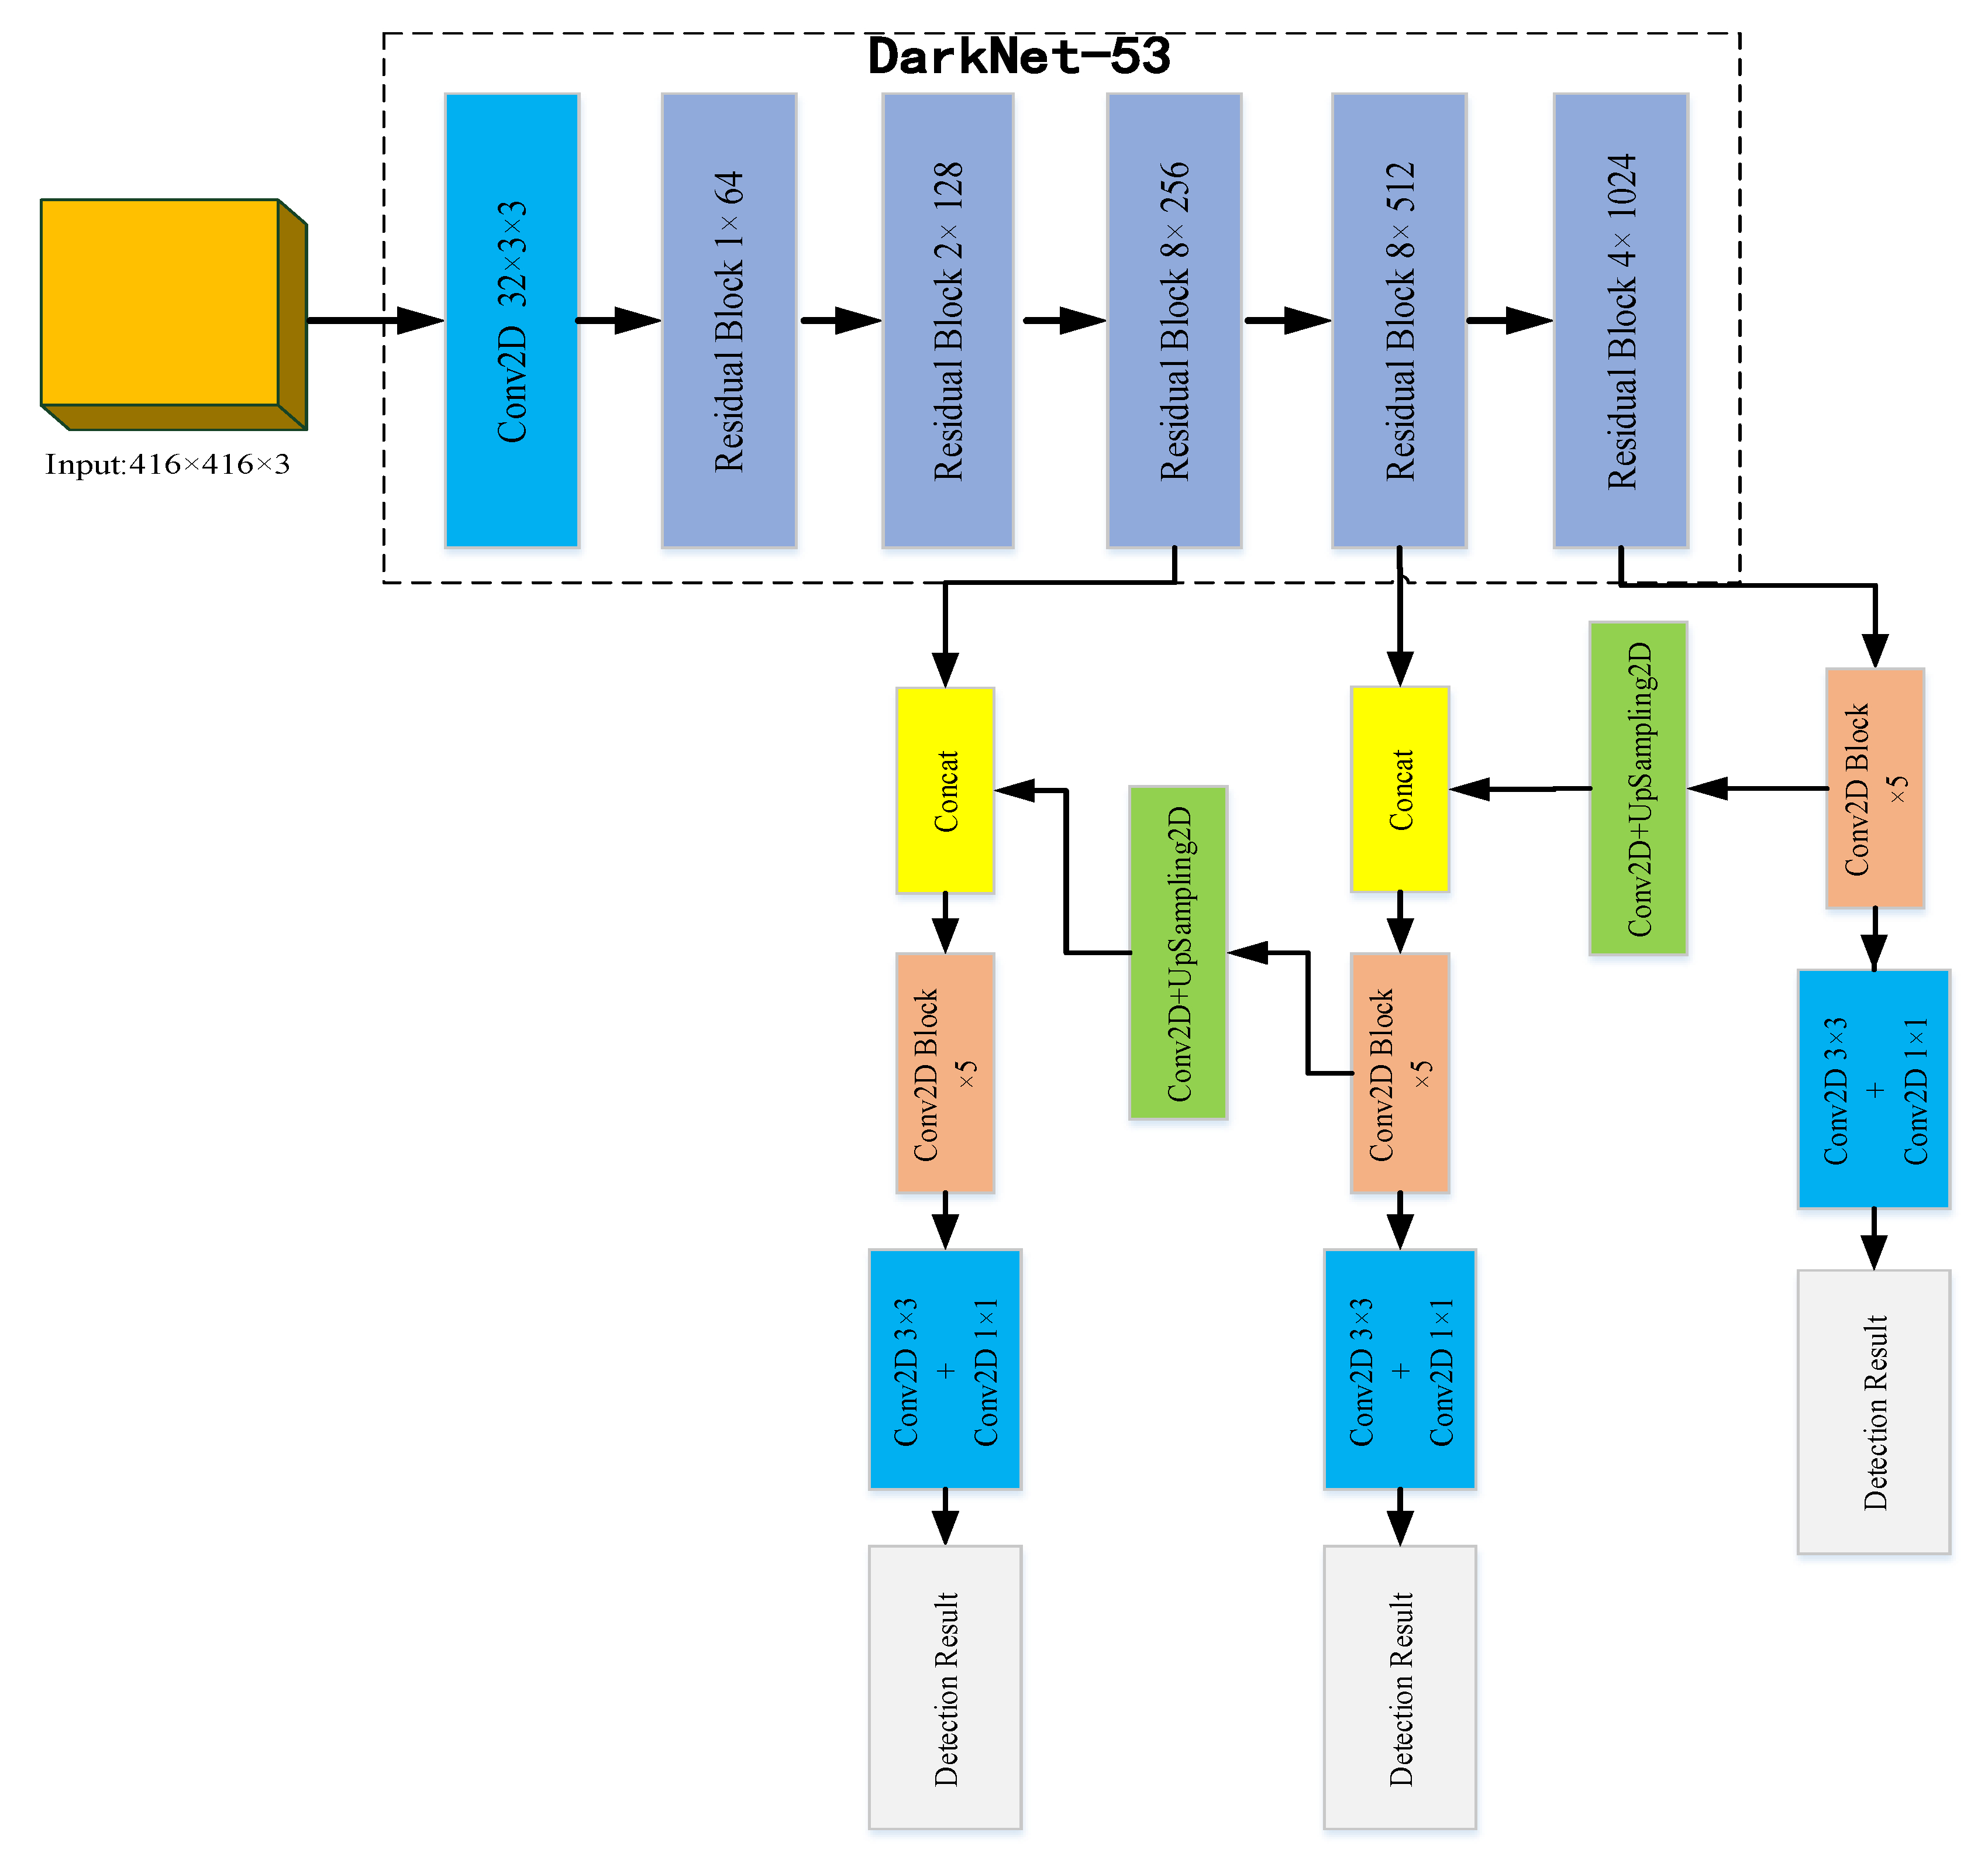
\includegraphics[width=0.6\textwidth]{images/2a-sign/YOLOv3-arch.jpg}
    \caption{Kiến trúc YOLOv3}
\end{figure}

\noindent Chính việc dự đoán với các scales khác nhau mà YOLOv3 đã cải thiện khi dự đoán các object nhỏ.

\noindent YOLOv3 vẫn sử dụng K-Means để chọn ra trước 9 prior boxes (anchor boxes). Đối với COCO dataset, width và height của mỗi anchor box là (10×13), (16×30), (33×23), (30×61), (62×45), (59× 119), (116 × 90), (156 × 198), (373 × 326).






\subsection{Áp dụng dataset cho bài toán}
Kiến trúc giải thuật mà nhóm sẽ sử dụng  gồm hai mô hình được xếp chồng lên nhau. Mô hình thứ nhất thực hiện nhiệm vụ xác định vị trí biển báo giao thông đang ở đâu trong bức ảnh được camera của xe ghi lại, có rất nhiều loại biển báo và sẽ được chia thành bốn loại lớn là:
\begin{itemize}
    \item Biến cấm: bao gồm các biển báo giao thông có hình tròn, nền trắng và viền đỏ. VD: giới hạn tốc độ, ... 
    \item Biển nguy hiểm: bao gồm các biển báo giao thông có hình tam giác, nền trắng và viền đỏ. VD: ngã tư, đường trơn trượt, ... 
    \item Biển bắt buộc : bao gồm các biển báo giao thông có hình tròn và nền màu xanh. VD: rẽ trái, rẽ phải, đi thẳng, ... 
    \item Các loại còn lại: bao gồm các biển báo giao thông không thuộc các danh mục trước đó. VD: đường ưu tiên, dừng lại, ... 
\end{itemize}
Sau khi dã xác định được vị trí của biển báo, hình ảnh sẽ được thu gọn lại vào bounding box của biển báo, sử dụng output của mô hình thứ nhất, điều chỉnh ảnh về kích thước 32x32 làm input cho mô hình thứ hai sử dụng mạng CNN và deep learning như đã đề cập ở trên để phân loại cụ thể đó là biển báo gì trong 43 lớp đã được xác định từ trước của bộ dataset. Như vậy, bằng việc sử dụng 2 lớp mô hình chồng lên nhau ta có thể giải quyết được vấn đề đặt ra.\\
Ta có thể tóm gọn lại kiến trúc cho bài toán phát hiện biển báo như sau:
\begin{figure}[htp]
    \centering
    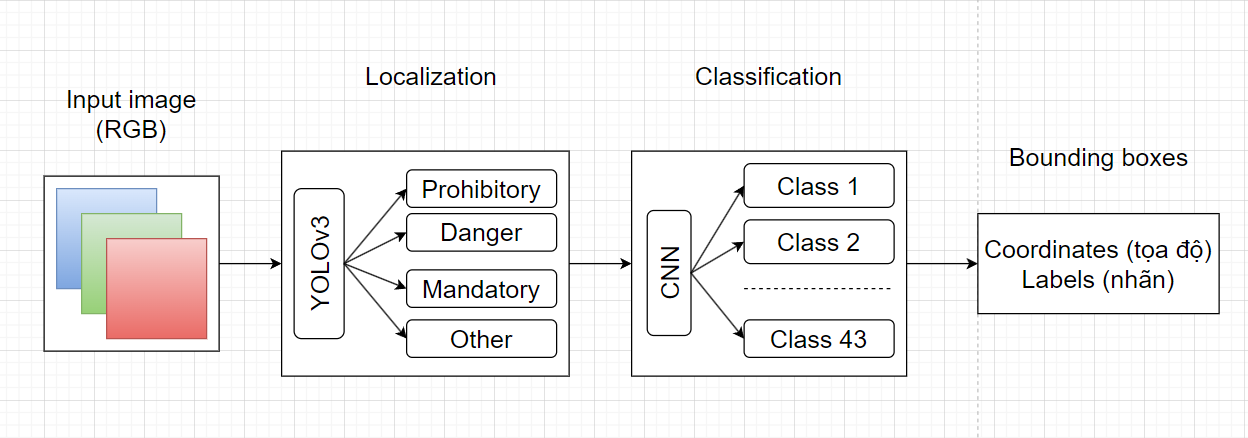
\includegraphics[width=0.8\textwidth]{images/2c-sign/sign-sys.png}
    \caption{Giải thuật}
    \label{fig:algo}
\end{figure}

\noindent Quay trở lại, ta đã đề cập là sẽ sử dụng hai bộ dữ liệu có sẵn là bộ biển báo giao thông của Đức GTSDB và GTSRB. Mô hình thứ nhất được huấn luyện trên bộ dữ liệu GTSDB (German Traffic Sign Detection Benchmark) gồm 900 bức ảnh đầu vào dạng RGB. Bộ dữ liệu bao gồm cả những hình ảnh không có biển báo giao thông để sử dụng trong quá trình huấn luyện. Tuy nhiên, quyết định đã được đưa ra để loại bỏ những hình ảnh này. Bộ dữ liệu kết quả đã được chia thành các tập con để huấn luyện và kiểm tra. \\
\newline
Nhãn cho các bounding box của từng hình ảnh được lưu trong 1 file txt như sau:

\begin{lstlisting}
00001.ppm;983;388;1024;432;40
00001.ppm;386;494;442;552;38
00001.ppm;973;335;1031;390;13
\end{lstlisting}
Thông số đầu tiên là tên bức ảnh, được lưu dưới dạng .ppm. Năm thông số tiếp theo lần lượt là: tọa độ góc trái, tọa độ góc phải, lớp (biển báo thuộc về lớp bao nhiêu trong 43 lớp đã xác định trước). Ví dụ:
\begin{lstlisting}[language = Python]
0 = speed limit 20 (prohibitory)
...
9 = no overtaking (prohibitory)
...
14 = stop (other)
...
31 = animals (danger)
33 = go right (mandatory)
34 = go left (mandatory)

\end{lstlisting}
Đầu tiên ta cần chuyển tất cả thông số này về định dạng mà YOLO dùng để huân luyện: tọa độ tâm x, tọa độ tâm y, chiều rộng và chiều cao của đối tượng, đồng thời chuẩn hóa các thông số về đoạn [0,1]. Sử dụng công thức như sau:
\begin{equation*}
    \begin{aligned}
        X_{centre} &= \frac{X_{min} + X_{max} }{2} \cdot \frac{1}{w}\\
        Y_{centre} &= \frac{Y_{min} + Y_{max} }{2} \cdot \frac{1}{h}\\
        width &= \frac{X_{max} - X_{min} }{2} \cdot \frac{1}{w}\\
        height &= \frac{Y_{max} - Y_{min} }{2} \cdot \frac{1}{h}\\
    \end{aligned}
\end{equation*}
Ta thu được các file .ppm được chuyển sang định dạng .jpg, với mỗi ảnh sẽ là một file.txt chứa các thông số được chuẩn hóa cho từng bounding box của biển báo:
\begin{figure}[htbp]
    \centering
    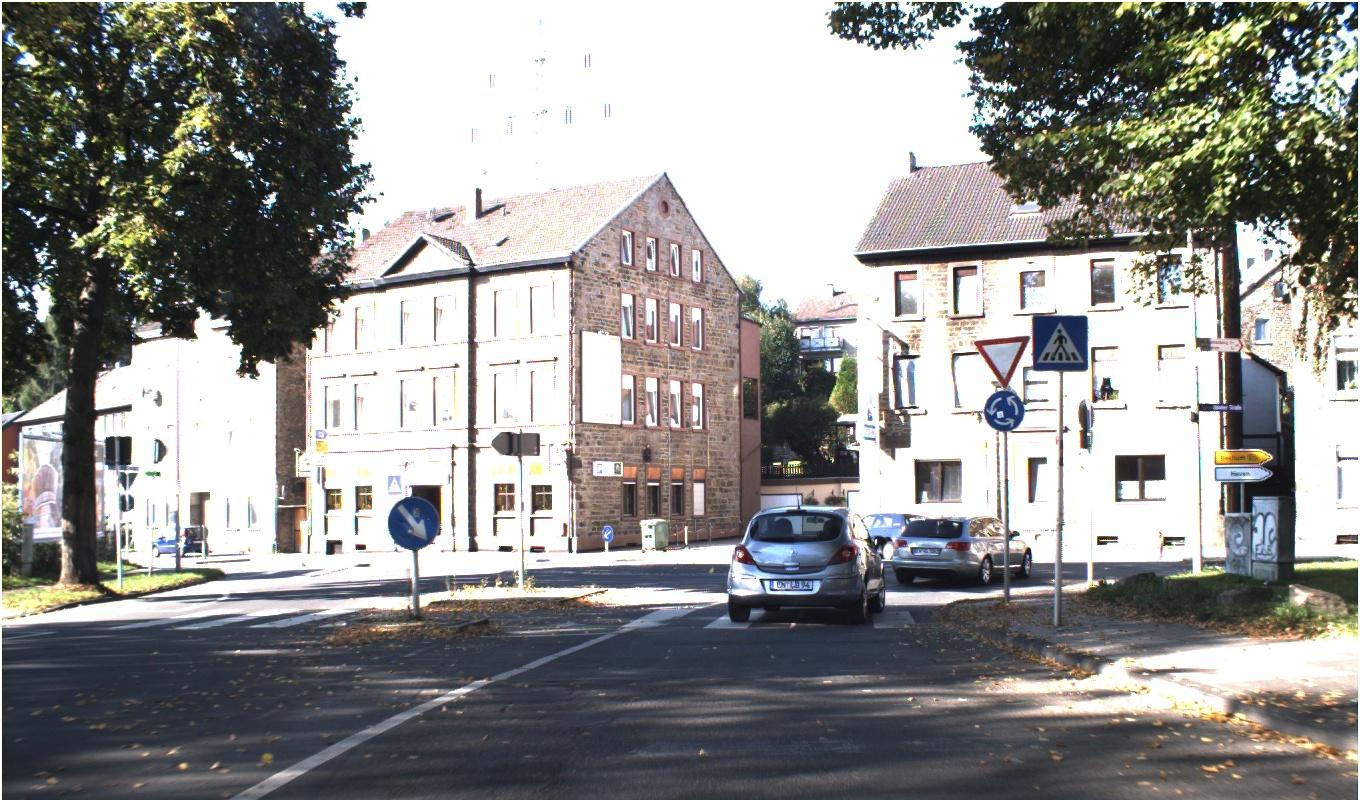
\includegraphics[width = 0.6\textwidth]{images/2c-sign/00001.jpg}
    \caption{Ảnh dataset}
\end{figure}
\begin{lstlisting}[language = Python]
#class X Y W H
2 0.7378676470588236 0.5125 0.030147058823529412 0.055
2 0.3044117647058823 0.65375 0.041176470588235294 0.0725
3 0.736764705882353 0.453125 0.04264705882352941 0.06875
\end{lstlisting}
Lúc này ta đã chuẩn bị đầy đủ dữ liệu để cho ra mô hình thứ nhất sử dụng YOLOv3.

\noindent Sau khi training xong và thu được file .weight với kết quả tốt nhất, ta tiếp tục đến với huấn luyện mô hình thứ hai - phân loại biển báo. \\
\newline 
Mô hình thứ hai được huấn luyện trên GTSRB với tổng cộng 66,000 hình ảnh RGB có dạng 32x32x3, gồm 43 loại biển báo mà ta đã đề cập đến ở phía trên. Ta có thể xem qua số lượng của từng loại biển báo như sau:
\newpage
\begin{figure}[htbp]
    \centering
    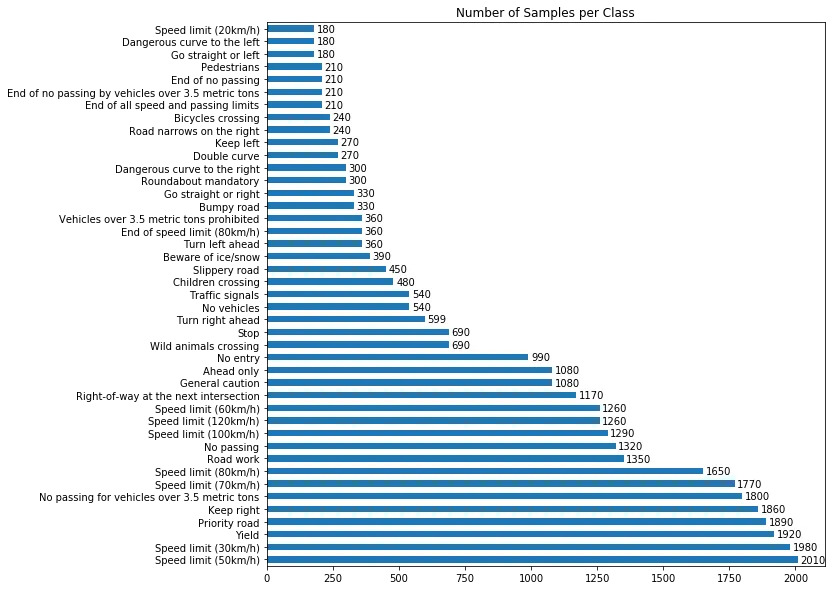
\includegraphics[width = 0.7\textwidth]{images/2c-sign/overall.jpg}
    \caption{Tổng quan GTSRB}
    \label{fig:overall}
\end{figure}

\noindent Tập dữ liệu này cũng sẽ chia thành nhiều phần với tý lệ nhất định cho ba mục đích gồm huấn luyện, kiểm tra và kiểm thử mô hình. Dựa vào \hyperlink{fig:overall}{\textcolor{blue}{hình}} trên ta thấy có sự chênh lệch không nhỏ giữa các biển báo khác nhau, vì thế trước khi huấn luyện cần làm thêm một bước là tăng cường dữ liệu:
\begin{lstlisting}[language = Python]
aug = ImageDataGenerator(rotation_range=0.18, 
                            zoom_range=0.15, 
                            width_shift_range=0.2, height_shift_range=0.2, 
                            horizontal_flip=True)
\end{lstlisting}

Sau khi huấn luyện cho mô hình thứ hai xong và nhận được kết quả như mong muốn, ta lưu model lại với định dạng .h5 để tiếp tục sử dụng. Dựa trên giải thuật đã trình bày trong \hyperlink{fig:algo}{\textcolor{blue}{hình}} ta cần tiền xử lí output của mô hình thứ nhất trước khi đưa nó vào làm input cho mô hình dự đoán thứ hai:
\begin{enumerate}
    \item \textbf{Gray-scale:} \\
    Do ảnh ban đầu có định dạng là RGB là một tập hợp gồm các điểm, mà mỗi điểm là bộ 3 màu red, green và blue, như vậy sẽ chứa các thông tin không cần thiết. Việc gray-scale giúp cho ta giảm bớt số lượng thông tin dư thừa, đồng thời phù hợp với model chúng ta train (lúc train model ta sử dụng ảnh gray-scale, nên khi ta predict ta cũng phải sử dụng ảnh gray-scale)
    \item \textbf{Sửa kích thước thành 32x32}\\
    Tùy thuộc vào vị trí đứng của xe, mà biển báo nhìn thấy được trong hình sẽ to hay nhỏ,
nên ta cần resize lại về cùng 1 kích thước. Khi đó ta mới có thể đem vào model.predict.
    \item \textbf{Local Histogram Equalization}\\
    Đây là phương pháp tăng độ tương phản cho ảnh khi ở dạng gray-scale. Nhờ vào phương
pháp này, ta có thể tăng độ chính xác khi predict.
\end{enumerate}
Về các biển báo cần nhận diện, trong chủ đề lần này, nhóm đã đề ra 1 số yêu cầu theo thứ tự ưu tiên để từ đó quyết định rằng tập dữ liệu cần thiết để giữ nguyên hay thay đổi số lượng của tập dữ liệu:
\begin{itemize}
    \item Tốc độ xử lý thời gian thực (Real-time processing)
    \item Độ chính xác cao (High precision)
\end{itemize}
Dựa trên hai tiêu chí này, nên trong quy mô của đồ án lần này model thứ hai sẽ bị lược bỏ bớt biển báo không cần thiết trong việc mô phỏng cũng như chạy kiểm thử, đồng thời chỉnh sửa một chút ở mô hình mạng CNN áp dụng để phù hợp hơn với số lượng mới cho tập dữ liệu. Như vậy, các biển báo nhóm sẽ sử dụng là:
\begin{itemize}
    \item Speed limit (60 km/h)
    \item Turn left ahead
    \item Turn right ahead
    \item Stop
\end{itemize}
Bằng cách này, tốc độ xử lí của xe trong mô phỏng cũng như hiệu suất dự đoán của mô hình sẽ nhanh và chính xác hơn. 
\subsubsection*{Kết quả thu được}
\newpage
\begin{itemize}
    \item \textbf{Speed limit (60 km/h)}
    \begin{figure}[htbp]
    \centering
    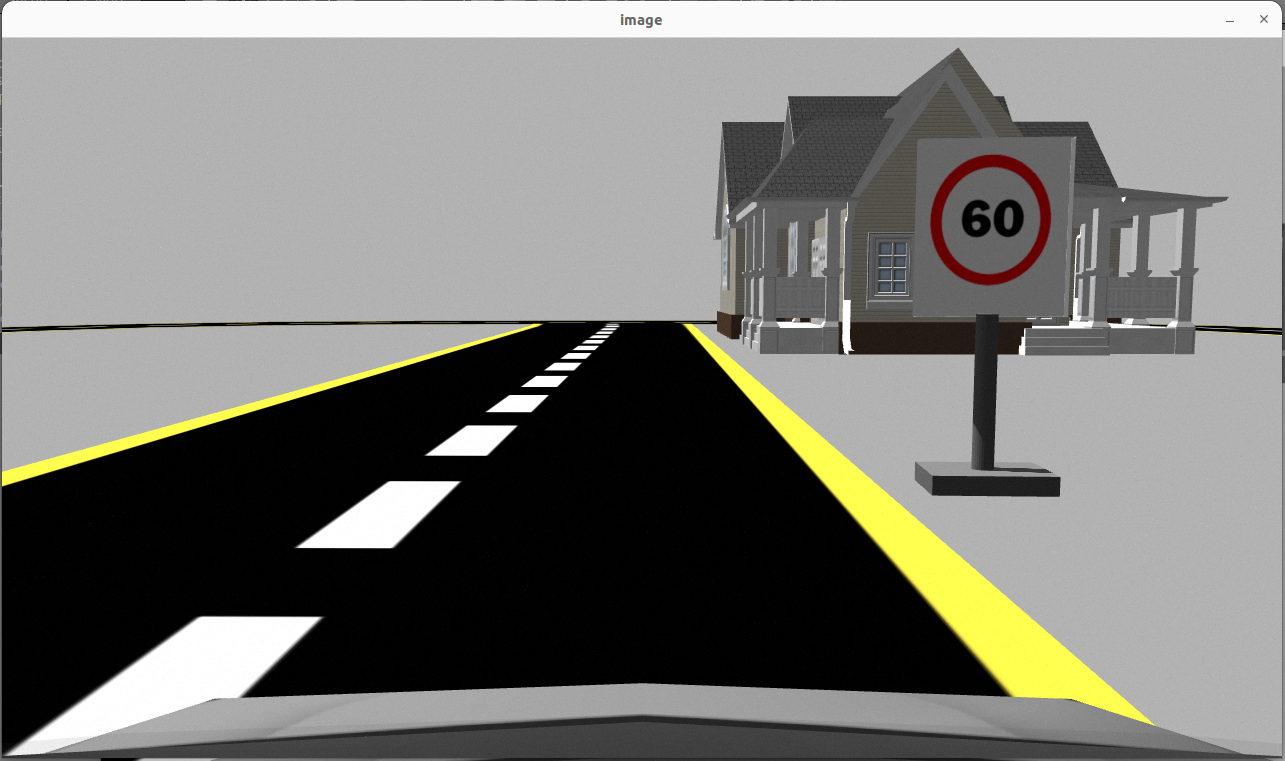
\includegraphics[width = 0.7\textwidth]{images/2c-sign/60-in.png}
    \caption{Input}
\end{figure}
    \begin{figure}[htbp]
    \centering
    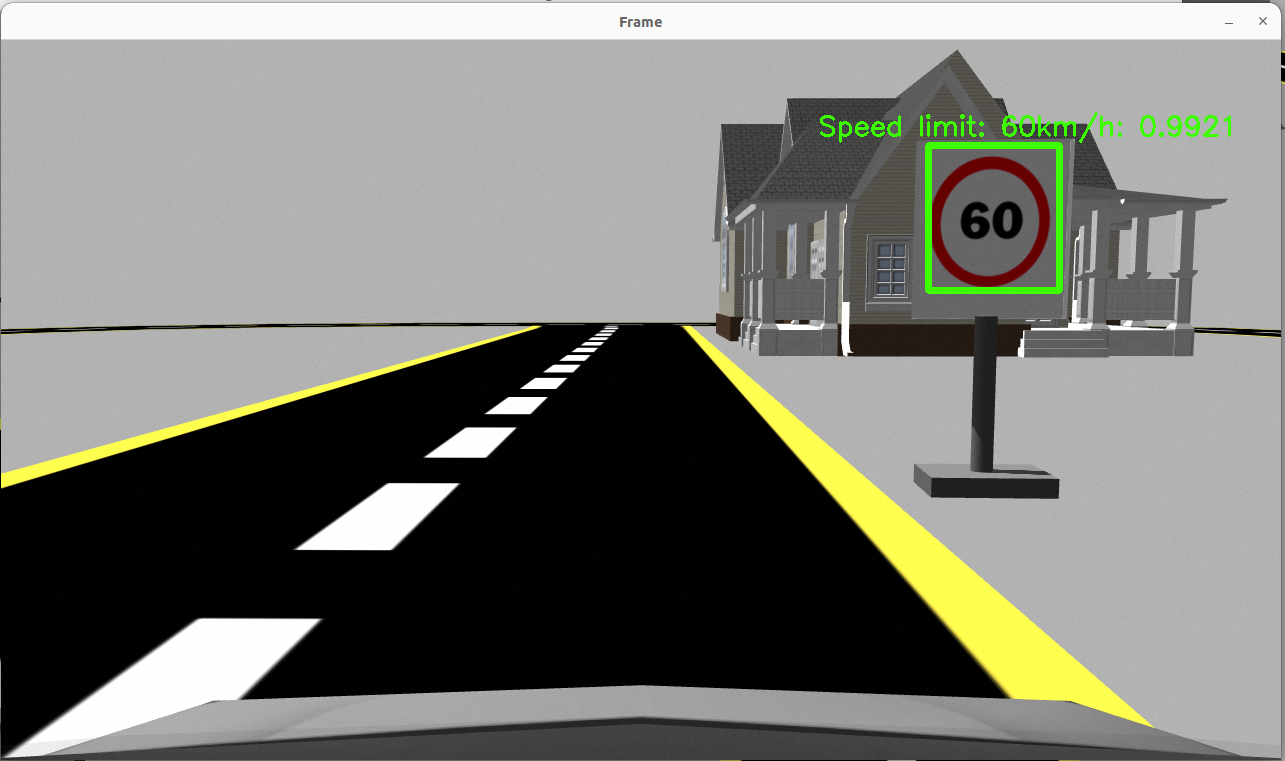
\includegraphics[width = 0.7\textwidth]{images/2c-sign/60-out.png}
    \caption{Output}
\end{figure}
\newpage
    \item \textbf{Turn left ahead}
    \begin{figure}[htbp]
    \centering
    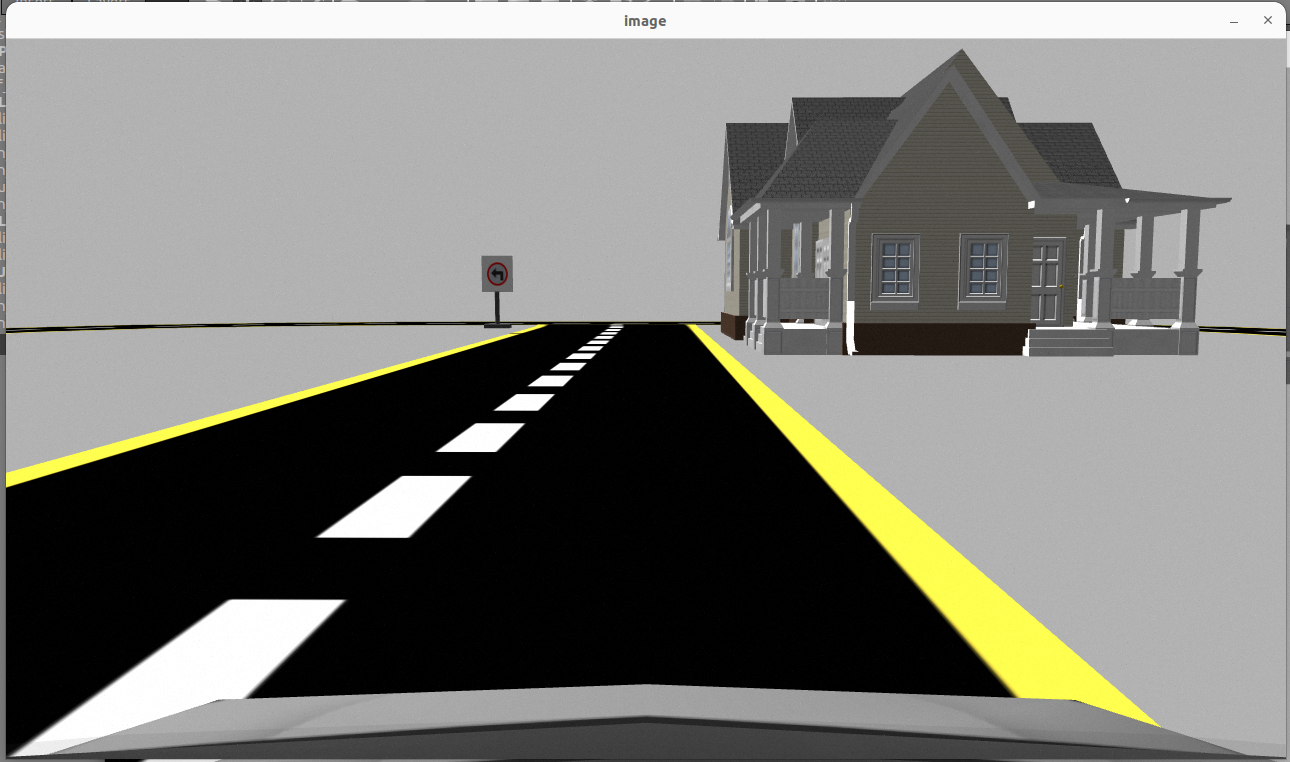
\includegraphics[width = 0.7\textwidth]{images/2c-sign/left-in.png}
    \caption{Input}
\end{figure}
    \begin{figure}[htbp]
    \centering
    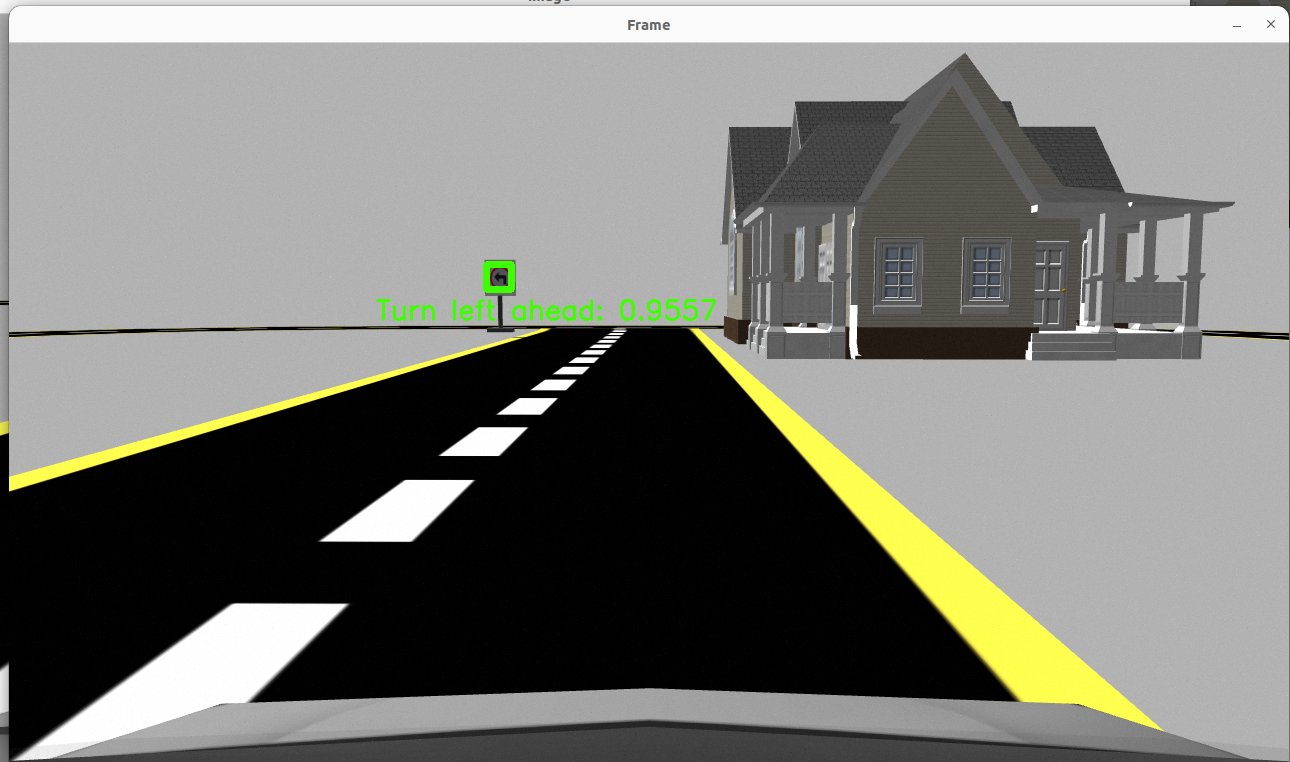
\includegraphics[width = 0.7\textwidth]{images/2c-sign/left-out.png}
    \caption{Output}
\end{figure}
\newpage
    \item \textbf{Stop}
    \begin{figure}[htbp]
    \centering
    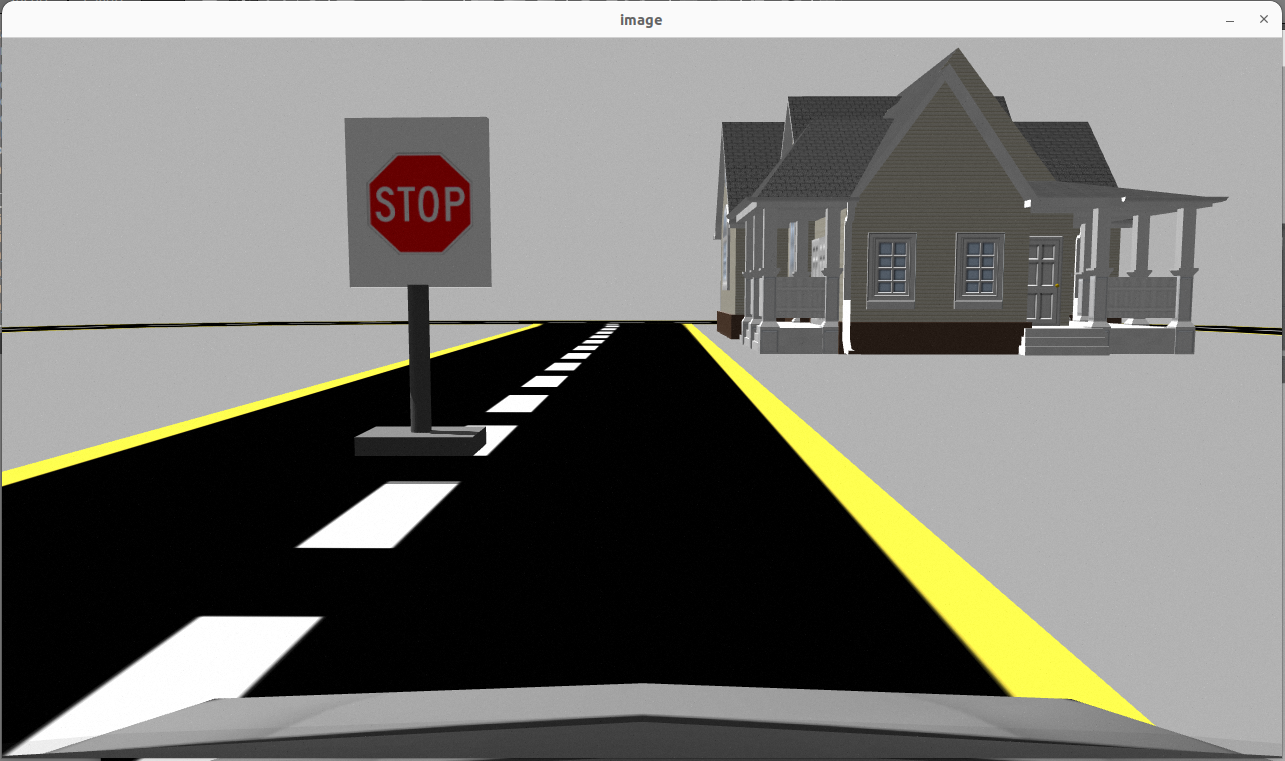
\includegraphics[width = 0.7\textwidth]{images/2c-sign/stop-in.png}
    \caption{Input}
\end{figure}
    \begin{figure}[htbp]
    \centering
    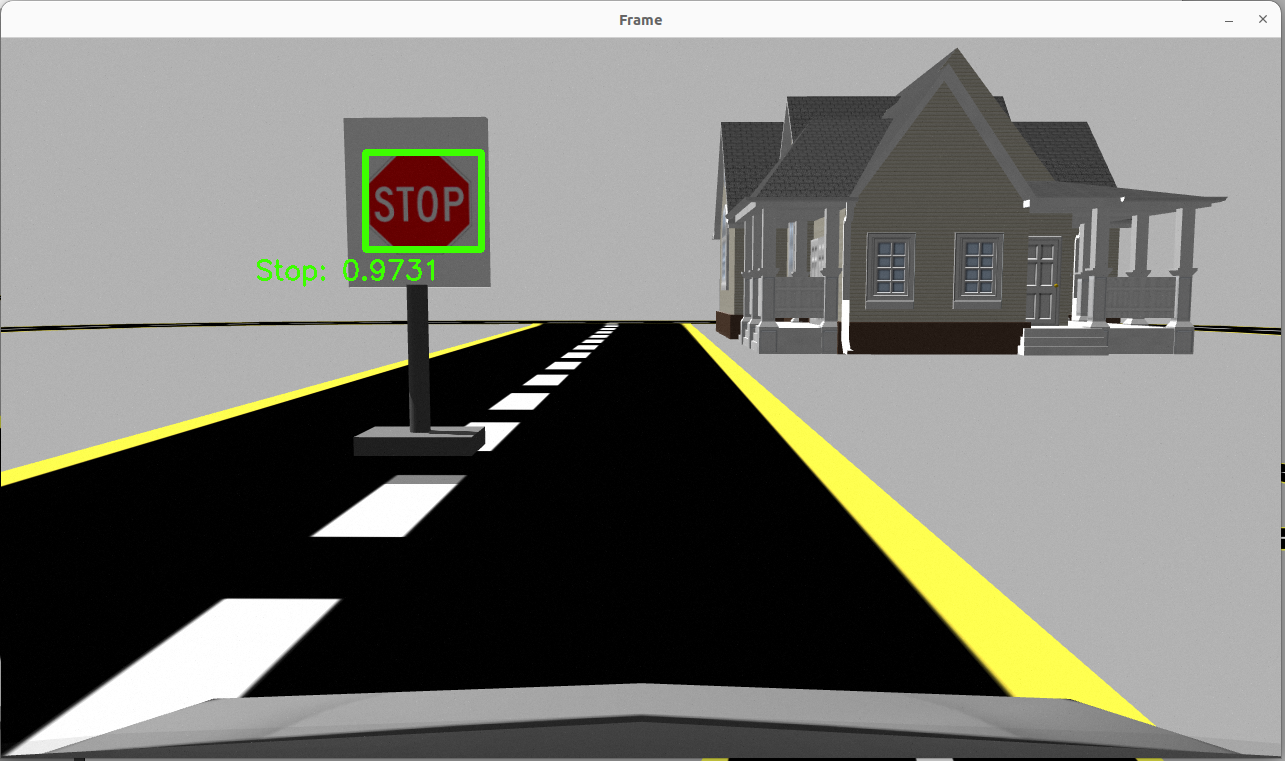
\includegraphics[width = 0.7\textwidth]{images/2c-sign/stop-out.png}
    \caption{Output}
\end{figure}
\end{itemize}
\newpage

\section{Bài toán nhận diện làn đường}
Trong bài toán lần này, nhóm sẽ đề xuất một giải thuật nhằm giúp xe phát hiện vị trí tương đối của bản thân chiếc xe và khoảng cách từ nó đến 2 vạch kẻ của làn đường. Mục đích của việc này là giúp xe có thể đưa ra những thông số về khoảng cách, độ lệch so với trung tâm hoặc phương hướng của làn đường (thẳng, cong) rồi từ đó bộ điều khiển sẽ tính toán và cân bằng ở chính giữa làn đường trong suốt thời gian di chuyển. Nhóm xin phép đề xuất một giải thuật như sau, tạm gọi là \textbf{giải thuật góc nhìn của chim (bird's eyes view algorithm)}. \\
\newline
Cụ thể, các bước cần thực hiện để hiện thực giải thuật như sau:
\begin{enumerate}
    \item \textbf{Hiệu chỉnh camera:}
    \begin{itemize}
        \item Sử dụng một tập hình ảnh bàn cờ vua chụp từ cùng một camera như ảnh đầu vào.
        \item Trả về tọa độ 4 góc của bàn cờ vua bằng các hàm của thư viện OpenCV.
        \item Sử dụng các góc phát hiện được để hiệu chỉnh camera và lấy ma trận hiệu chỉnh camera cùng các hệ số méo.
    \end{itemize}

    \item \textbf{Điều chỉnh méo ảnh:}
    \begin{itemize}
        \item Áp dụng ma trận hiệu chỉnh camera và các hệ số méo để sửa chữa méo ống kính trong ảnh gốc.
    \end{itemize}

    \item \textbf{Phân ngưỡng ảnh:}
    \begin{itemize}
        \item Sử dụng các biến đổi màu sắc, độ dốc và các kỹ thuật khác để tạo ra ảnh nhị phân dựa trên ngưỡng.
        \item Các phương pháp ngưỡng có thể bao gồm ngưỡng độ dốc, ngưỡng màu (ví dụ, trong không gian màu HLS hoặc LAB) và ngưỡng thích ứng.
    \end{itemize}

    \item \textbf{Biến đổi góc nhìn:}
    \begin{itemize}
        \item Áp dụng một biến đổi góc nhìn để có được "góc nhìn từ trên cao" của làn đường.
        \item Xác định các điểm nguồn và đích cho biến đổi góc nhìn.
        \item Sử dụng các hàm getPerspectiveTransform và warpPerspective của OpenCV.
    \end{itemize}

    \item \textbf{Phát hiện làn đường và điều chỉnh điểm làn:}
    \begin{itemize}
        \item Xác định điểm làn bằng cách sử dụng các kỹ thuật như đỉnh lịch sử hoặc cửa sổ trượt.
        \item Điều chỉnh một đa thức để biểu diễn biên giới của làn đường được phát hiện.
    \end{itemize}

    \item \textbf{Ước lượng độ cong làn đường:}
    \begin{itemize}
        \item Tính toán cong đường của làn đường được điều chỉnh bằng các công thức toán học phù hợp.
        \item Xác định vị trí của xe so với trung tâm của làn đường.
    \end{itemize}

    \item \textbf{Điều chỉnh làn trở lại:}
    \begin{itemize}
        \item Điều chỉnh biên giới của làn đường được phát hiện trở lại trên ảnh gốc bằng cách sử dụng biến đổi góc nhìn nghịch đảo.
    \end{itemize}

    \item \textbf{Hiển thị:}
    \begin{itemize}
        \item Xuất hiển thị hình ảnh của biên giới làn đường trên ảnh gốc bao gồm các ước lượng số liệu về đường cong và vị trí của xe.
    \end{itemize}
\end{enumerate}
\newline 
Như vậy, có thể hiểu đây là một quá trình chuyển đổi góc nhìn 2D từ camera quay trở lại điểm nhìn thật trong thế giới 3D thật vốn có. Trong giải thuật này, quá trình hiệu chỉnh camera là một bước quan trọng để khắc phục méo ảnh từ góc độ hình ảnh, đặc biệt là khi camera nhìn vào các đối tượng 3D trong thế giới thực và chuyển đổi chúng thành một ảnh 2D trên mặt phẳng hình ảnh. Méo ảnh có thể làm thay đổi hình dạng và kích thước của đối tượng trong quá trình này, ảnh hưởng đến khả năng nhận dạng làn đường.\\
\newline
Tóm tắt lại, ta có quy trình hiện thực giải thuật như sau:
\begin{figure}[htbp]
    \centering
    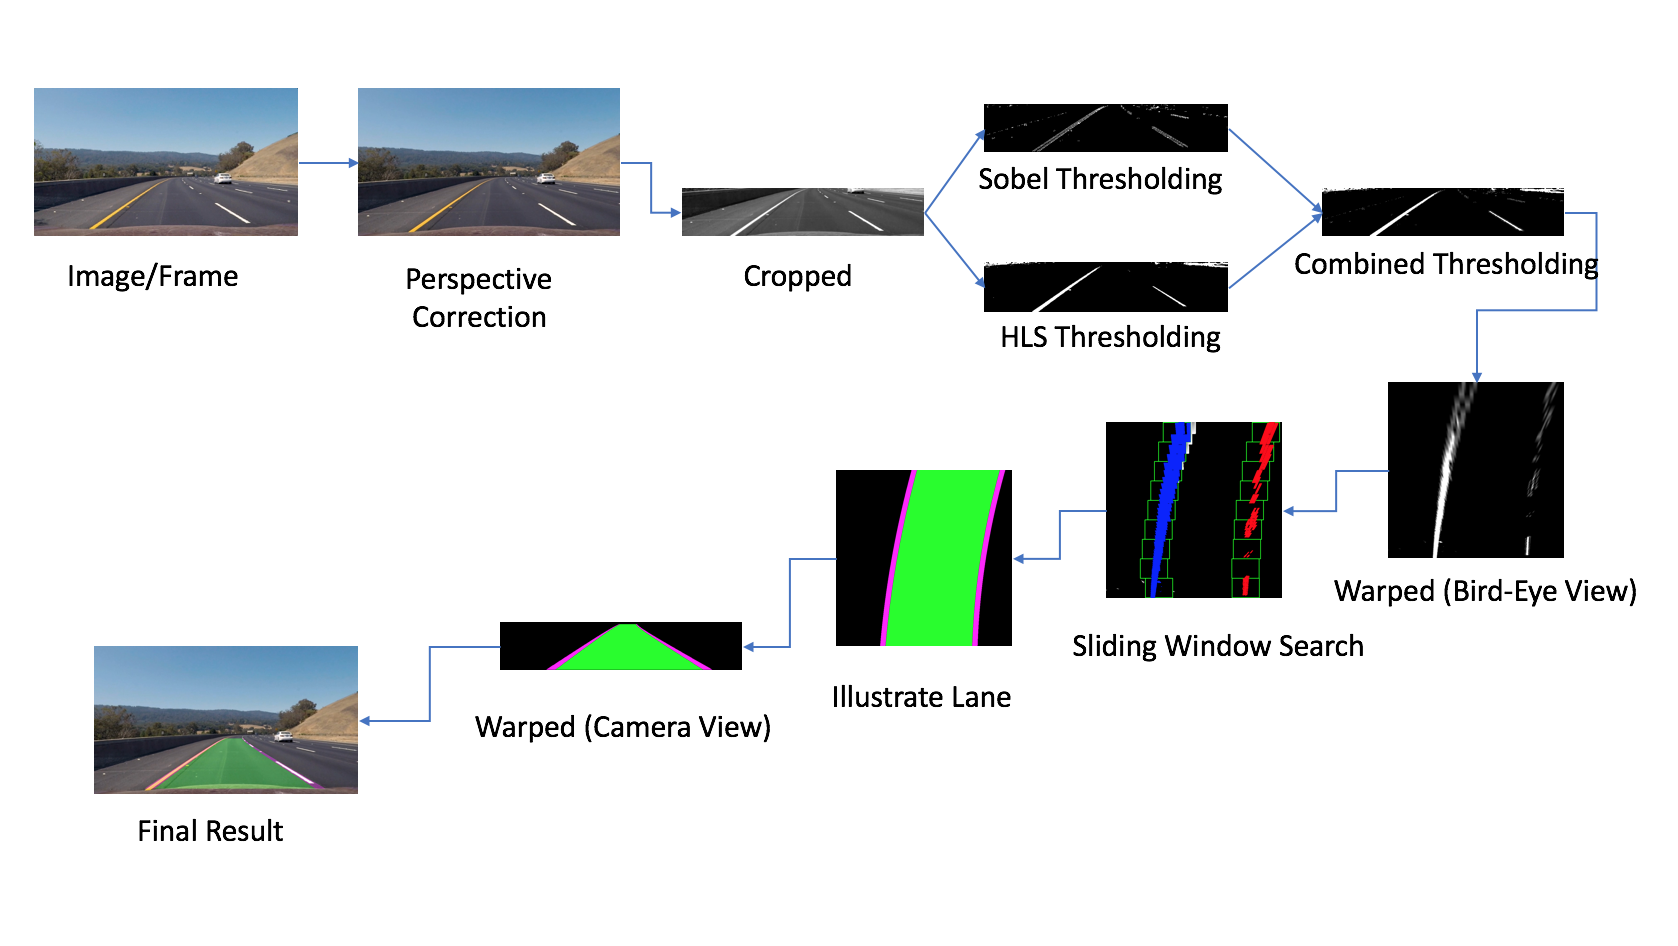
\includegraphics[width = 0.8\textwidth]{images/3-lane/pipeline.png}
    \caption{Bird's eyes view}
\end{figure}
\newline 
Sau đây, ta sẽ đi sau hơn vào từng phần đồng thời giải thích rõ hơn phương pháp và giải thuật mà nhóm đang sử dụng.

\subsection{Hiệu chỉnh camera (camera calibration)}
Quá trình chụp ảnh thông qua ống kính có thể tạo ra sự méo lệch đáng kể trong hình ảnh. Có hai loại méo lệch chính, đó là méo lệch tâm cầu và méo lệch tiếp xúc. Hiện tượng méo ảnh xảy ra khi camera quan sát các đối tượng có đặc tính 3D trong thế giới thực và muốn chuyển chúng thành mặt phẳng 2D trên ảnh. Thực tế, quá trình chuyển đổi này không thể hiệu quả và gây ra nhiều méo ảnh trong hình ảnh, làm thay đổi hình dạng và kích thước của đối tượng trong quá trình chuyển đổi. Do đó, việc đánh giá mức độ méo ảnh của hình ảnh được coi là bước tiền xử lý quan trọng. Thực tế, bước này ảnh hưởng đáng kể đến hiệu suất của việc phát hiện làn đường, vì hình ảnh bị méo sẽ làm cho làn đường trong một số phần trở nên cong và đưa ra khỏi ứng dụng phát hiện từ thực tế. Nó cũng làm cho hình ảnh trông nghiêng, khiến cho một số đối tượng trông xa hơn hoặc gần hơn so với thực tế.
\newpage
\begin{figure}[htbp]
    \centering
    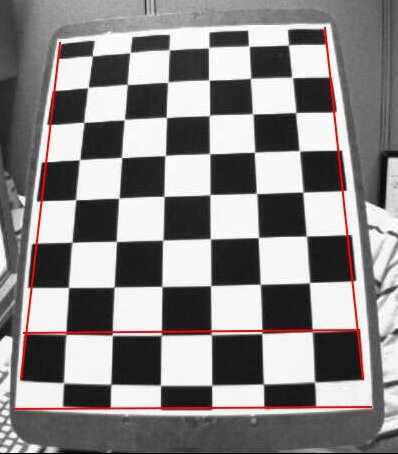
\includegraphics[width = 0.4\textwidth]{images/3-lane/calib_radial.jpg}
    \caption{Hiện tượng lệch ảnh}
\end{figure}
Trong đó:
\begin{itemize}
    \item (x,y) là tọa độ của một điểm trong hình ảnh bị méo.
    \item $(x_{distorted},y_{distorted})$ là tọa độ tương ứng của điểm đã được làm phẳng sau khi được sửa chữa.
    \item r là khoảng cách từ trung tâm của hình ảnh đến điểm (x,y).
    \item $k_1, k_2, k_3$ là các hệ số méo lệch tâm cầu xác định mức độ méo lệch tâm cầu.
\end{itemize}
\noindent Độ méo lệch tâm cầu có thể được biểu diễn như sau:
\begin{equation*}
    \begin{aligned}
        x_{distorted} &= x(1 + k_1 r^2 + k_2 r^4 + k_3 r^6)\\
        y_{distorted} &= y(1 + k_1 r^2 + k_2 r^4 + k_3 r^6)
    \end{aligned}
\end{equation*}

\noindent Tương tự, méo lệch tiếp xúc xảy ra vì ống kính chụp ảnh không được căn chỉnh hoàn hảo song song với mặt phẳng hình ảnh. Do đó, một số khu vực trong hình ảnh có thể trông gần hơn so với dự kiến. Số lượng méo lệch tiếp xúc có thể được biểu diễn như sau:
\begin{equation*}
    \begin{aligned}
        x_{distorted} &= x + [2 p_1 x y + p_2(r^2 + 2x^2)]\\
        y_{distorted} &= y + [p_1 (r^2 + 2 y^2) + 2 p_2 x y]
    \end{aligned}
\end{equation*}

\noindent Tóm lại, chúng ta cần xác định năm tham số, được gọi là các hệ số méo lệch, theo công thức:
\begin{center}
    Distortion coefficients = ($k_1$, $k_2$, $p_1$, $p_2$, $k_3$)
\end{center}

\noindent Tiêu cự và quang tâm có thể được sử dụng để tạo ra ma trận camera, từ đó có thể loại bỏ méo lệch do ống kính của một camera cụ thể. Ma trận camera là duy nhất đối với một camera cụ thể, vì vậy khi tính toán một lần, nó có thể được sử dụng lại trên các hình ảnh khác chụp bởi cùng một camera. Ma trận này được biểu diễn dưới dạng ma trận 3 x 3: 
\[
Camera Matrix = 
\left[
\begin{array}{ccc}
    f_x & 0 & c_x \\
    0 & f_y & c_y \\
    0 & 0 & 1
\end{array}
\right]
\]
Các bước thực hiện hiệu chỉnh ảnh như sau:
\begin{enumerate}
    \item Chuẩn bị "điểm vật", là các tọa độ (x, y, z) của các góc của bảng cờ vua trong thế giới thật. Điều này giả sử bảng cờ vua được cố định trên mặt phẳng (x, y) ở z = 0. Đồng thời, giả sử kích thước của mô hình bảng cờ vua giống nhau cho tất cả các hình ảnh, nên "điểm vật" sẽ giống nhau cho mỗi hình ảnh hiệu chỉnh.
    \item Tiếp theo, hình ảnh hiệu chỉnh được nạp tuần tự, chuyển đổi sang ảnh xám (gray scale), và tìm kiếm mô hình bảng cờ vua bằng \textbf{cv2.findChessboardCorners}. Khi mô hình được tìm thấy, vị trí của các góc được làm sáng cường thêm để đạt được độ chính xác sub-pixel bằng cách sử dụng \textbf{cv2.cornerSubPix}. Điều này nâng cao độ chính xác của hiệu chỉnh. Tọa độ của góc được thêm vào danh sách chứa tất cả các điểm ảnh, trong khi "đối tượng" được chuẩn bị được thêm vào danh sách chứa tất cả các "điểm vật".
    \item Hệ số méo (distortion coefficients )và ma trận camera (camera matrix) được tính toán bằng cách sử dụng hàm \textbf{cv2.calibrateCamera()}, trong đó hình ảnh và điểm "đối tượng" được chuyển làm đầu vào. Quan trọng là kiểm tra xem kết quả có đạt được không, vì hiệu chỉnh là một quy trình số học phi tuyến tính, nên nó có thể tạo ra kết quả không tối ưu. Để làm điều này, hình ảnh hiệu chỉnh được đọc một lần nữa và đưa ra sự méo ảnh. Hình ảnh đã được làm phẳng được hiển thị để kiểm tra mắt xem sự méo ảnh đã được sửa chữa hay chưa. Sau khi dữ liệu đã được kiểm tra, các tham số được đóng gói và lưu vào tệp. Một ví dụ về hình ảnh đầu vào, hình ảnh với góc của bảng cờ vua và hình ảnh đã được làm phẳng được hiển thị.
\end{enumerate}
\begin{table}[h]
    \centering
    \begin{tabular}{|c|c|c|}
        \hline
        \rowcolor[gray]{0.9}
        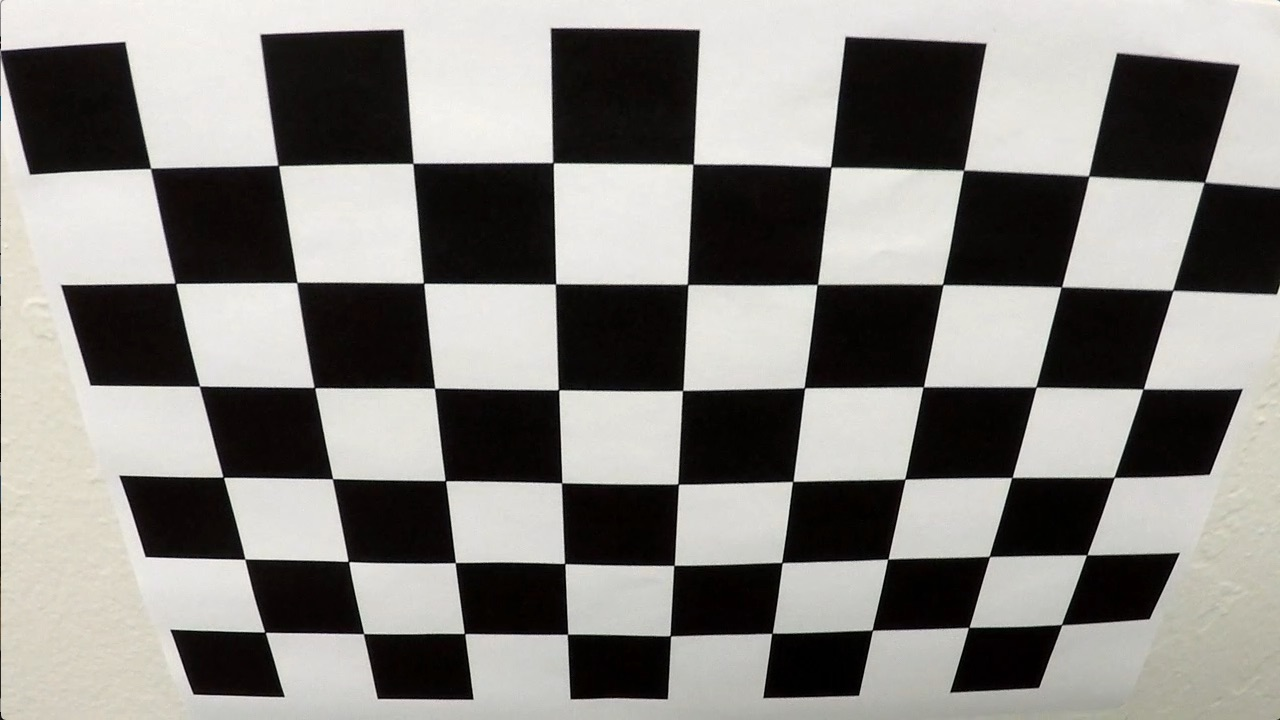
\includegraphics[width=0.3\linewidth]{images/3-lane/o.jpg} & 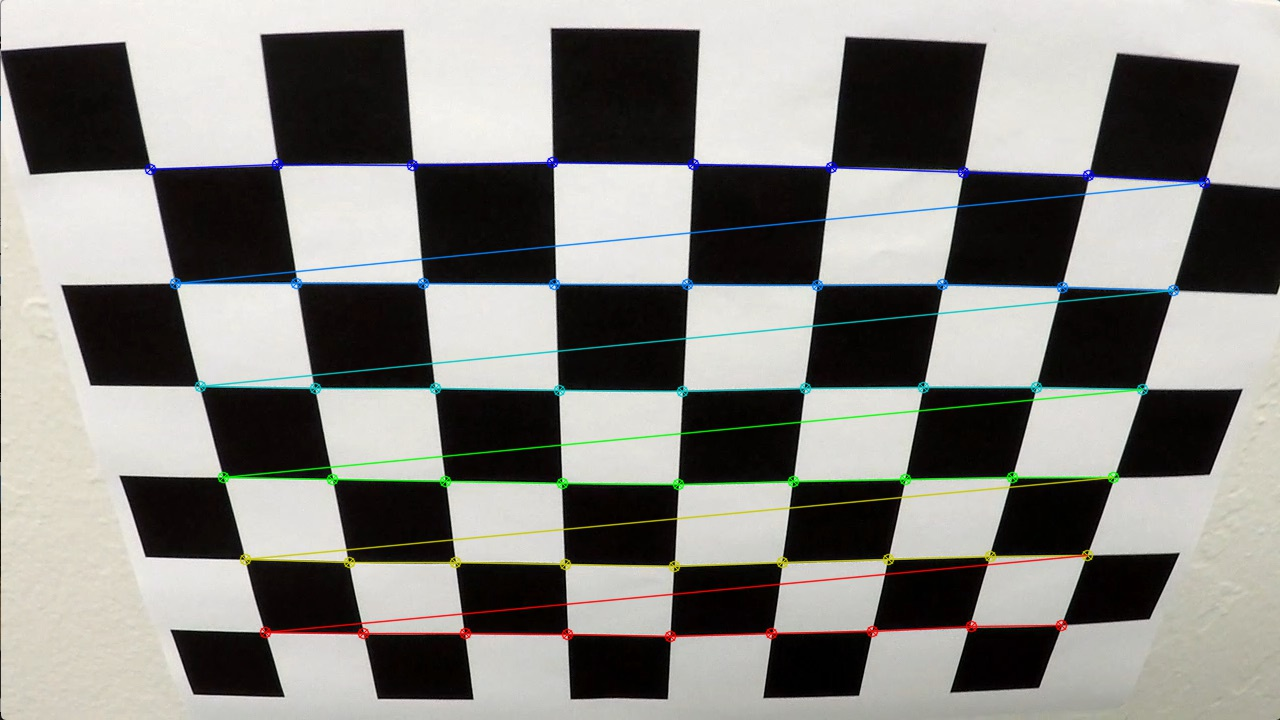
\includegraphics[width=0.3\linewidth]{images/3-lane/c.jpg} & 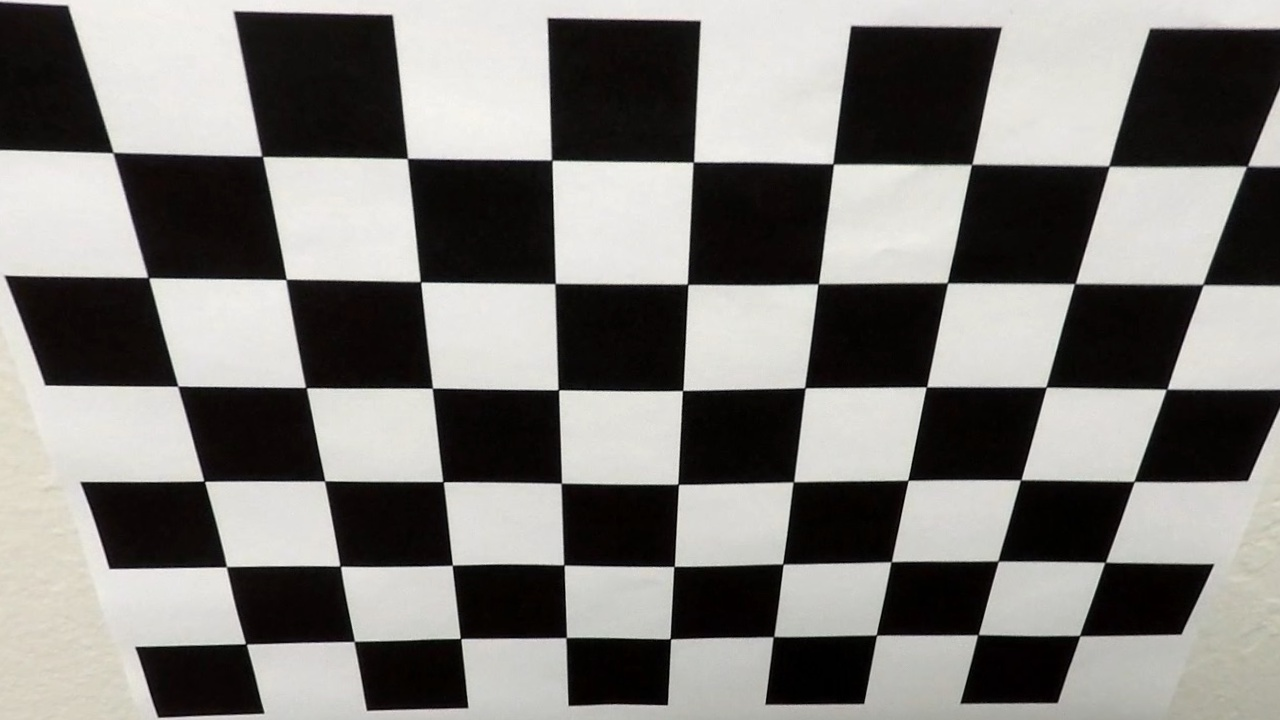
\includegraphics[width=0.3\linewidth]{images/3-lane/u.jpg} \\
        \hline
        \rowcolor[gray]{0.9}
        \textbf{Original image} & \textbf{Chessboard corners} & \textbf{Undistorted image} \\
        \hline
        \rowcolor[gray]{0.9}
    \end{tabular}
        \caption{Hiệu chỉnh ảnh trên bàn cờ vua}
\end{table}

\noindent Ma trận camera bao gồm mô hình camera "lỗ khóa" (pinhole) trong đó. Nó cung cấp mối quan hệ giữa tọa độ của các điểm liên quan đến camera trong không gian 3D và vị trí của điểm đó trên hình ảnh theo đơn vị pixel. Nếu X, Y và Z là tọa độ của điểm trong không gian 3D, vị trí của nó trên hình ảnh (u và v) theo đơn vị pixel được tính bằng cách sử dụng:
\newline
\begin{equation*}
    \begin{aligned}
        \left[
    \begin{array}{c}
    \\
         u  \\
         v  \\
         1
    \end{array}   
\right]
&= sM
\left[
    \begin{array}{c}
    
         X  \\
         Y  \\
         Z
    \end{array}   
\right]
    \end{aligned}
\end{equation*}
Trong đó M đại diện cho ma trận camera, và ss là một hệ số vô hướng khác không bằng không. Phương trình này sẽ được sử dụng sau này.
\newpage
\subsection{Áp dụng hiệu chỉnh ảnh}
Áp dụng hiệu chỉnh ảnh, ta thu được hình ảnh trước và sau khi sử dụng trên như sau:
\begin{figure}[htbp]
    \centering
    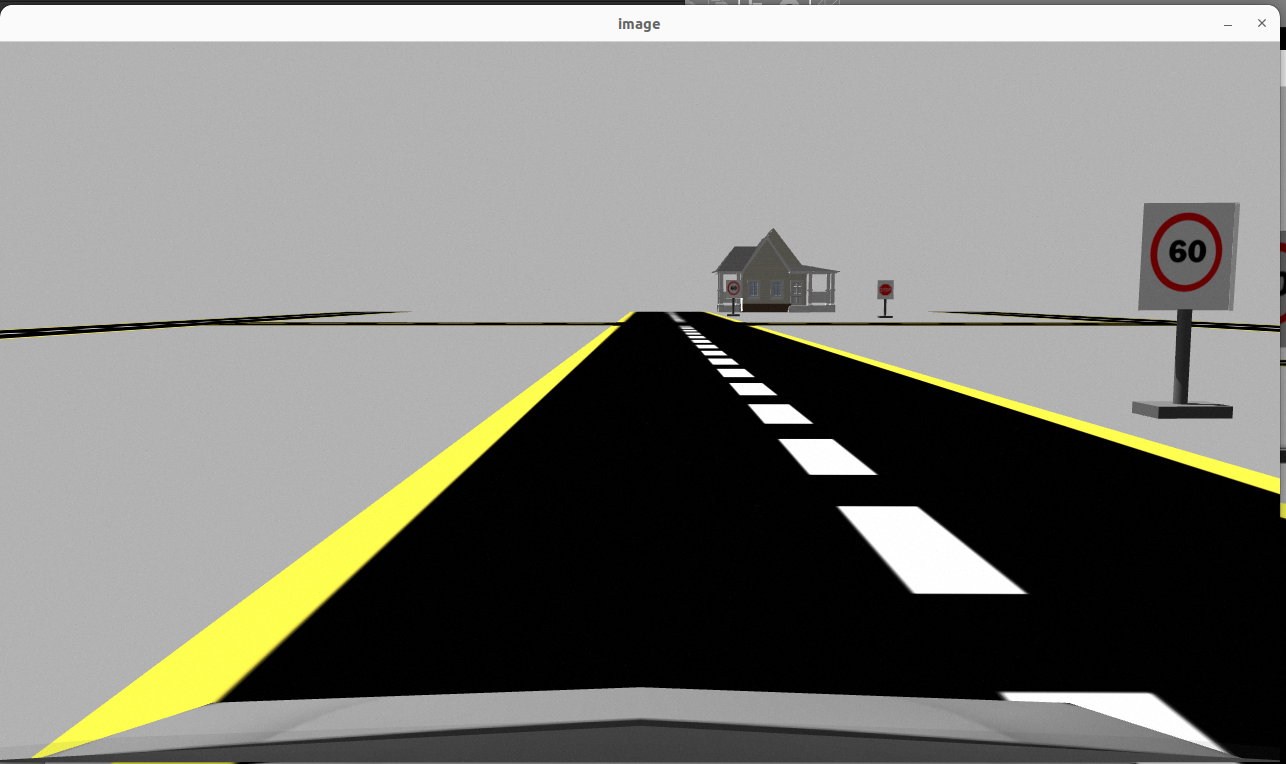
\includegraphics[width=0.6\linewidth]{images/3-lane/d._img.png}
    \caption{Trước hiệu chỉnh}
\end{figure}
\begin{figure}[htbp]
    \centering
    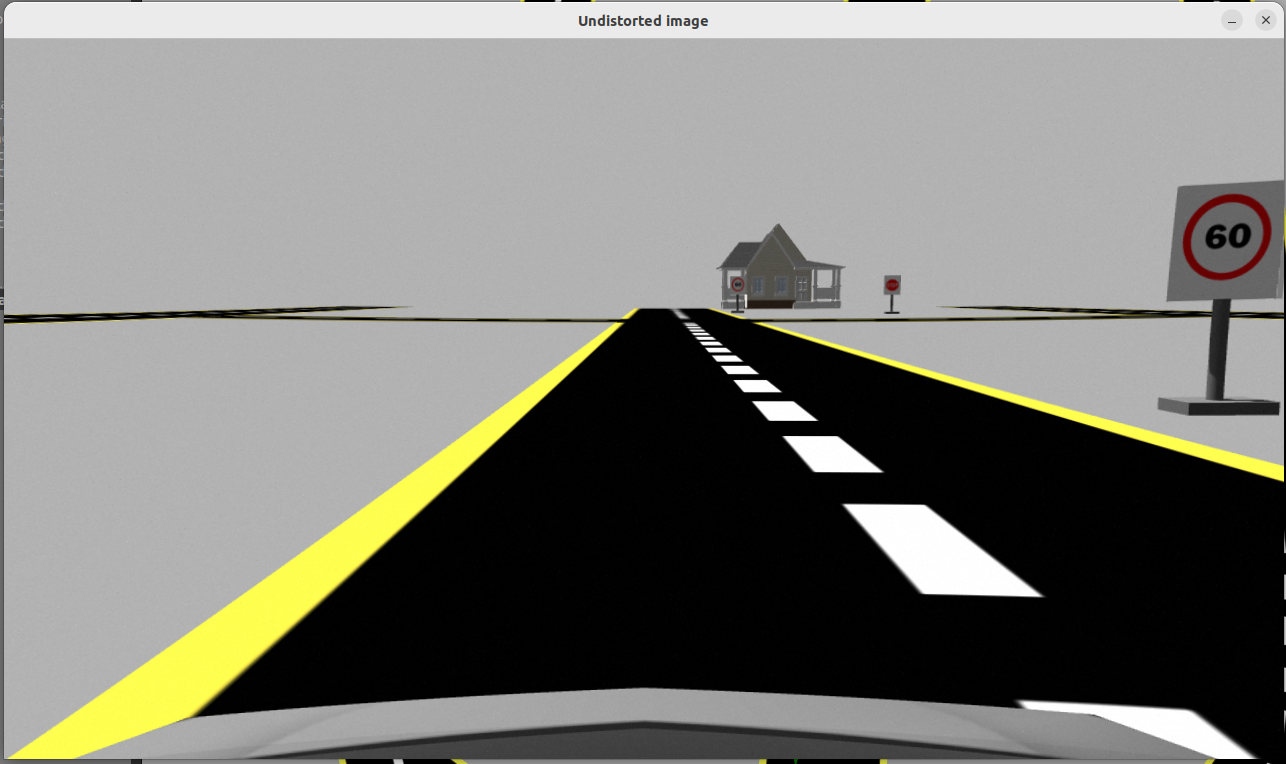
\includegraphics[width=0.6\linewidth]{images/3-lane/u._img.png}
    \caption{Sau hiệu chỉnh}
\end{figure}

\noindent Có thể ngay lúc này, khi nhìn vào bức ảnh đã được hiệu chỉnh, ta vẫn chưa thấy sự khác biệt quá lớn lao nào so với bức ảnh đầu vào, tuy nhiên việc này sẽ tăng hiệu quả cũng như độ chính xác trong việc áp dụng các giải thuật về sau.

\subsection{Phân ngưỡng ảnh}
\subsubsection{Edge và Gradient}
\subsubsection*{Edge}
Trong ảnh số, những điểm ảnh có cường độ ảnh sáng thay đổi mạnh so với các điểm xung quanh thường được gọi là các điểm cạnh (edge point). Cạnh (edge) là tập hợp các điểm cạnh tạo nên một hình dạng có ý nghĩa nào đó liên quan đến thông tin hình dạng và cấu trúc của đối tượng trong ảnh, ví dụ đường bao của một khuôn mặt, cấu trúc vành mũ, ... Tách cạnh là quá trình trích rút các thông tin tin cạnh bằng các phép toán xử lý ảnh.\\
Ví dụ như ta có một bức ảnh và ta lấy một đường kẻ ngang rồi ta sẽ lấy mức xác theo đường thằng đó, ta sẽ thấy được sự thay đổi mức xám ở các vị trí. \\

\begin{figure}[htbp]
    \centering
    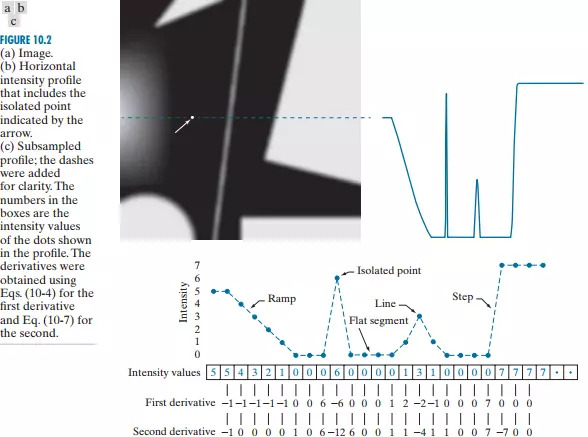
\includegraphics[width=0.5\linewidth]{images/3-lane/edge.jpg}
\end{figure}
\subsubsection*{Gradient}
Khi nhắc đến sự thay đổi đổi thì ta thường nhắc tới Gradient. Gradient của hàm cho biết hàm tăng mạnh như thế nào.\\
Ví dụ với hàm 1 chiều: $f(x) = x^2$ thì Gradient của nó được ký hiệu và tính như sau: $$\nabla f(x) = \frac{\partial f(x)}{\partial x} = 2x$$
\begin{itemize}
    \item Grad(2) = 4 chỉ ra hướng tăng của hàm là bên phải
    \item Grad (-1) = -2 chỉ ra hướng tăng của hàm nằm ở bên trái.
\end{itemize}
Gradient không chỉ tính bằng đạo hàm bậc 1, ta cũng thể tính bằng đạo hàm bậc. Với độ biến đổi của mức sáng bên trên ta tính được đạo hàm bậc 1, bậc 2 và công thức tương ứng như sau: 
\begin{figure}[htbp]
    \centering
    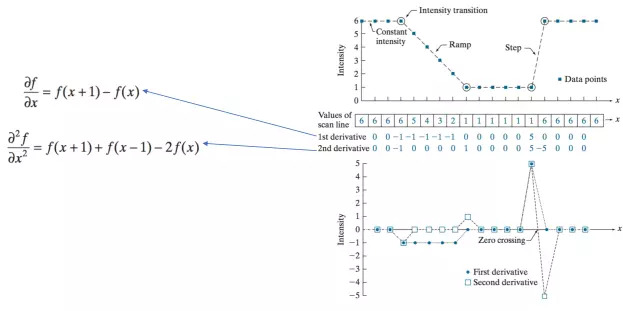
\includegraphics[width=0.5\linewidth]{images/3-lane/gradgrad.jpg}
\end{figure}
\newpage
\subsubsection{Phát hiện cạnh sử dụng đạo hàm}
Ta có bức ảnh đã được hiệu chỉnh trong phần trước:\\

\begin{figure}[htp]
    \centering
    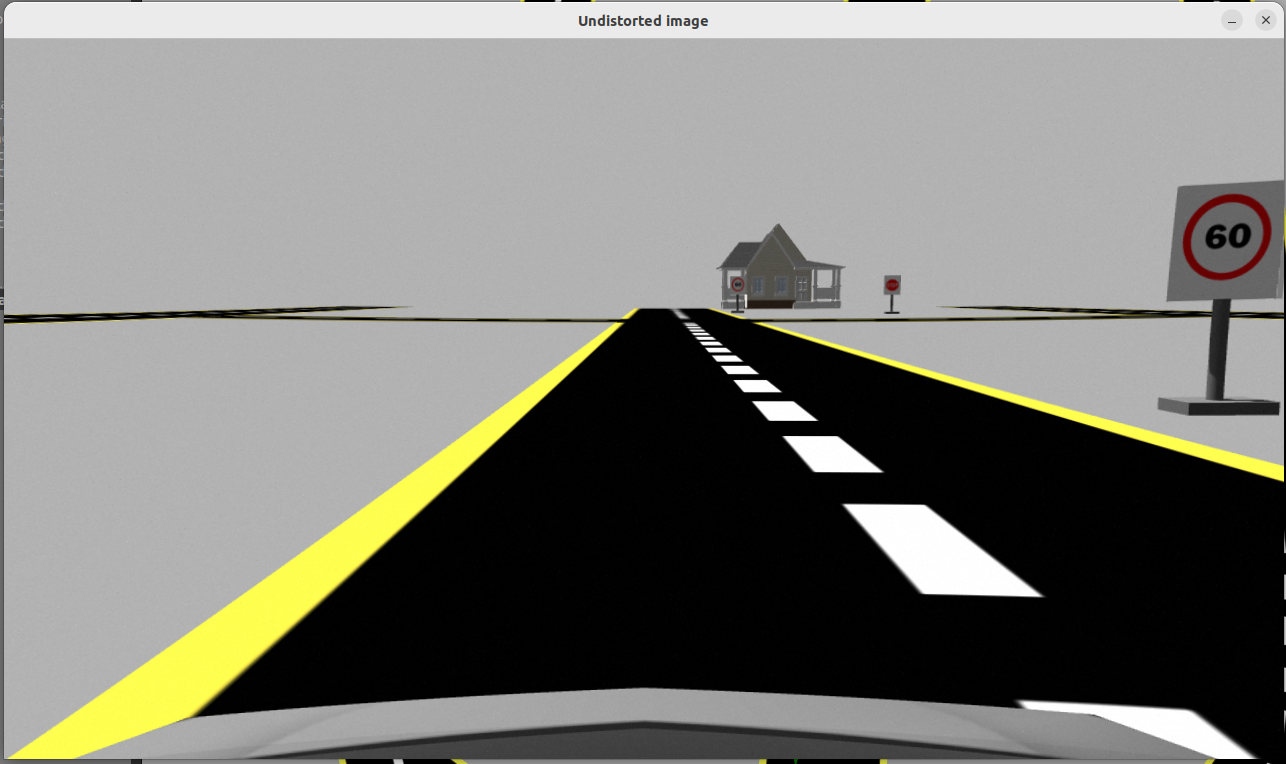
\includegraphics[width=0.4\linewidth]{images/3-lane/u._img.png}
    \caption{Ảnh đã hiệu chỉnh}
\end{figure}
\noindent Có thể sử dụng đạo hàm để phát hiện biên cạnh hoặc đường viền của làn đường trong hình ảnh, đặc biệt là khi màu sắc của đường và nền có sự tương phản cao. Trong hệ màu RGB, mỗi điểm ảnh có thể được biểu diễn bằng ba giá trị tương ứng với mức độ đỏ (R), xanh lá cây (G), và xanh dương (B). Sự thay đổi nhanh chóng trong giá trị này có thể tương ứng với sự thay đổi trong màu sắc, cho phép chúng ta phát hiện được các đường biên.

\noindent Một cách phổ biến để phát hiện cạnh là sử dụng đạo hàm của ảnh. Đạo hàm có thể được tính theo nhiều cách, nhưng một cách phổ biến là sử dụng bộ lọc Sobel hoặc Scharr. 

\noindent Như đã nói ở trên, có hai cách để phát hiện cạnh sử dụng đạo hàm:
\begin{itemize}
    \item Phát hiện giá trị cực tiểu hoặc cực đại địa phương trong đạo hàm bậc 1
    \item Phát hiện zero-crosssing (chính là chỗ giá trị từ âm sang dương hoặc ngược lại bạn có thể nhìn chú thích ở hình trên) trong đạo hàm bậc 2.
\end{itemize}

% \begin{figure}[htbp]
%     \centering
%     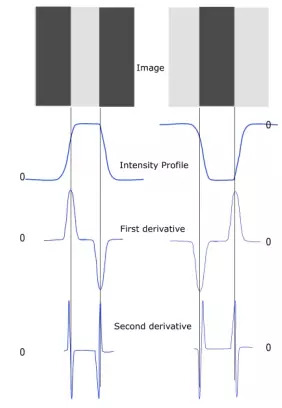
\includegraphics[width=0.3\linewidth]{images/3-lane/deri.jpg}
% \end{figure}

\noindent Đạo hàm trong không gian 2 chiều được tính như sau:
\[
    \nabla f(x,y) = \frac{\partial f(x,y)}{\partial x} \Vec{i} + \frac{\partial f(x,y)}{\partial y} \Vec{j}
\]
Tuy nhiên để áp dụng trong xử lí ảnh, việc xấp xỉ hóa đạo hàm của hàm rời rạc là cần thiết. Xấp xỉ đạo hàm bậc nhất hàm gradient được tính như sau (1), ở đây giá trị nhỏ nhất trong ảnh là 1 pixel:
\[
\frac{\partial f(x,y)}{\partial x} = f(x+1,y) - f(x,y)
\]
\[
\frac{\partial f(x,y)}{\partial y} = f(x,y+1) - f(x,y)
\]
Độ lớn của gradient cho biết cường độ của cạnh tại điểm đó:
\[
|\nabla f(x,y)| = \sqrt{\left( \frac{\partial f(x,y)}{\partial x}\right)^2 + \left(\frac{\partial f(x,y)}{\partial y}\right)^2}
\]
Trong xử lí ảnh, ta có các bước để tính gradient như sau:
\begin{itemize}
    \item Gradient theo cột
    \item Gradient theo hàng
    \item tổng hợp hai Gradient trên
\end{itemize}
Nếu chúng ta sử dụng phương pháp thông thường để tính gradient bằng cách duyệt từng hàng và cột của ma trận, quá trình này thường mất nhiều thời gian tính toán. Để tối ưu hóa quá trình này, có một số phương pháp và kỹ thuật hiện đại mà chúng ta có thể áp dụng.\\
Một trong những cách là sử dụng phép tính gradient thông qua các phép toán ma trận và kernel mà chúng ta đã học từ bài trước. Thay vì duyệt qua từng phần tử của ma trận và tính gradient riêng lẻ, chúng ta có thể sử dụng các phép toán ma trận để thực hiện tính toán này một cách hiệu quả hơn.\\
Cụ thể, ta có thể sử dụng phép tích chập (convolution) với kernel đã được học trước đó để áp dụng tính toán gradient cho toàn bộ ma trận một cách đồng thời. Điều này giúp giảm thiểu số lượng phép toán cần thực hiện và tăng tốc quá trình tính gradient.\\
Với việc sử dụng phép toán kernel và kỹ thuật convolution, chúng ta không chỉ giảm thời gian tính toán mà còn tận dụng được hiệu suất của các thư viện và trình tối ưu hóa ma trận hiện đại, giúp tăng cường khả năng tính toán của thuật toán gradient trong bài toán của chúng ta.

\subsubsection{Áp dụng phương pháp để phân ngưỡng ảnh}
Có khá nhiều kernel thông dụng được sử dụng cho việc phát hiện biên và cạnh, cũng như có một số phương pháp hiện đại có thể dùng cho việc này(có thể kể đến giải thuật Canny), nhóm nhận định rằng với tính chất cũng như yêu cầu về sự cân bằng giữa tốc độ xử lí và độ chính cao cao, nên sẽ chọn \textbf{Sobel kernel}, vừa đơn giản hóa các thông tin mà máy chủ cần xử lí, đồng thời vẫn đảm bảo được độ chính xác cao.\\
Sobel kernel:
\[\frac{1}{4}
\left[
    \begin{array}{ccc}
        1 & 0 & -1  \\
        2 & 0 & -2 \\
        1 & 0 & -1
    \end{array}
\right]
\]

Như vạy, sau khi xử dụng Sobel kernel để lọc bức ảnh đầu vào, ta thu được:

\begin{figure}[htbp]
    \centering
    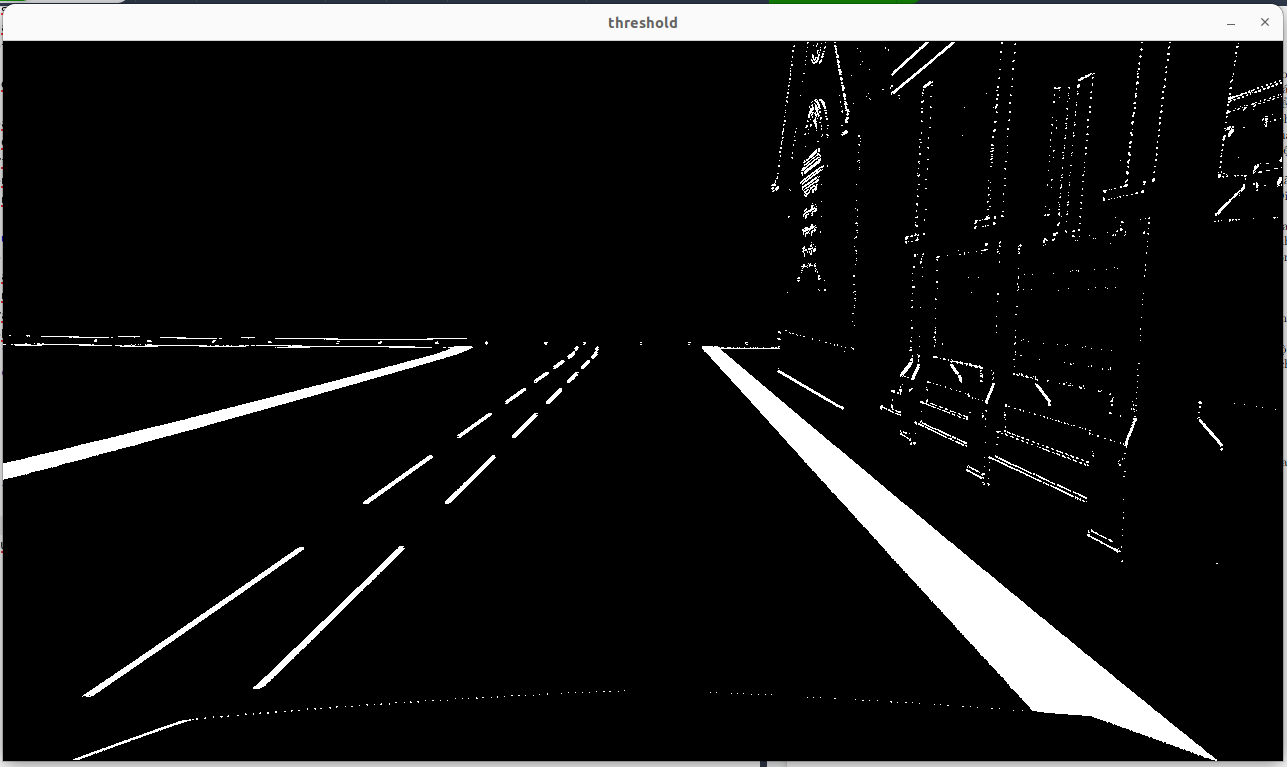
\includegraphics[width=0.8\linewidth]{images/3-lane/threshold.png}
    \caption{Phân ngưỡng ảnh}
\end{figure}

Với việc làn đường màu trắng và vàng, là những màu có cường độ lớn, ta đã thu được hình ảnh trong đó những đường kẻ nối liền bên tay phải và các đường nét đứt bên trái đều là cạnh và làn đường mà ta đã phát hiện được.

\subsection{Chuyển góc nhìn (get perspective transform)}
Tiếp theo, ta sẽ tiến hành việc thay đổi góc nhìn của ô tô đối với làn đường. Ta cũng thấy, trong hình ảnh mà camera thu nhận, làn đường không phải là hai đường thẳng song song mà lại là hai đường thẳng giao nhau ở phía xa của bức ảnh. Như vậy, việc đánh giá tính chất của làn đường (thẳng, cong trái, phải ..) là rất khó khắn, vì vậy ta sẽ tiến hành chuyển đổi góc nhìn của ô tô sang như thể đang nhìn vuông góc từ trên trời xuống.\\
Các bước được dùng để tiến hành đổi góc nhìn như sau:
\begin{enumerate}
    \item Chọn ma trận đến, ma trận đích 
    \item Tính toán ma trận dùng để biến đổi từ ma trận đầu thành ma trận cuối và ngược lại (sử dụng \textbf{cv2.getPerspectiveTransform}
    \item Thay đổi bức ảnh đầu vào bằng \textbf{cv2.warpPerspective} và xuất ra kết quả.
\end{enumerate}
Lưu ý, vì ta đang xử lí trên ảnh nên ma trận bốn điểm là một ma trận 4 x 2 vì đây là không gian 2D. Đồng thời các điểm này phải nằm trong độ lớn giới hạn của khung hình là 1280 x 720 (pixel). Sau khi thực thi ta thu được kết quả sau:\\
%
Với bức ảnh đầu vào:\begin{figure}[htbp]
    \centering
    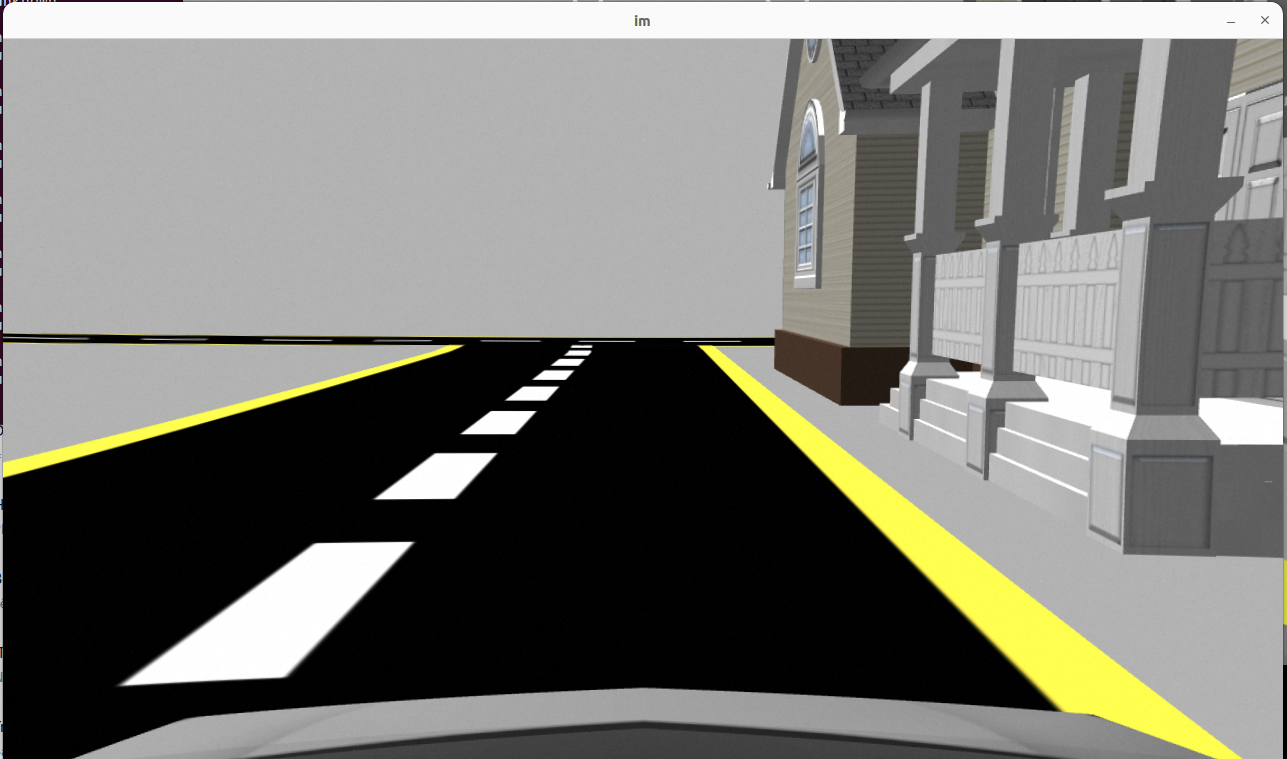
\includegraphics[width=0.4\linewidth]{images/3-lane/ori.png}
    \caption{Đầu vào}
\end{figure}
ta được:
\begin{figure}[htbp]
    \centering
    \subfigure[]{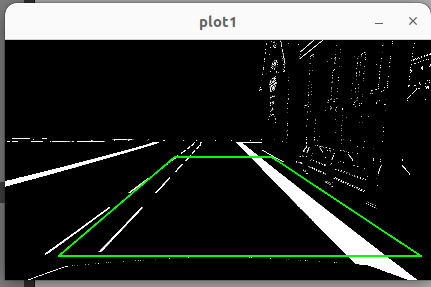
\includegraphics[width=0.4\linewidth]{images/3-lane/plot1.png}}
    \subfigure[]{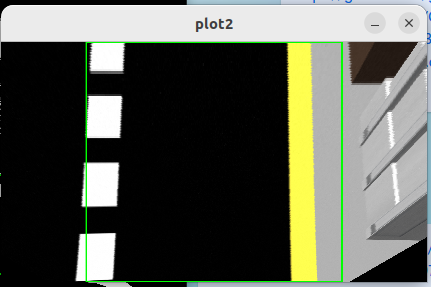
\includegraphics[width=0.4\linewidth]{images/3-lane/plot2.png}}
    \caption{Đổi góc nhìn}
\end{figure}

\noindent Như vậy, giải thuật thay đổi tầm nhìn của ô tô, cộng với việc đã phân ngưỡng ảnh trước đó, bức ảnh thu được gần như đã hiển thị rõ phàn mà ta gọi là làn đường cũng như loại bỏ những thông tin không cần thiết về các vật thể khác nhau xuất hiện trên đường. Tiếp theo ta sẽ sử dụng một số phép tính toán để có thể vẽ ra một đường thẳng (hoặc cong) có thế chưa gần hết từng bên của làn đường dể có thể thực hiện tính toán cân bằng. 

\subsection{Nhận diện làn đường}
Có thể thấy được trên hình, phần làn đường không chỉ đơn giản là những pixel đơn rời rạc được nối lại với nhau tạo thành một đường thẳng hay cong, mà bao gồm một vùng pixel gồm các pixel có độ lớn tương đồng nhau. Để có thể vẽ ra được một làn đường phù hợp, ta sẽ sử dụng phương pháp của sổ trượt (sliding window search). Tóm tắt quy trình sử dụng phương pháp này như sau:
\begin{enumerate}
    \item \textbf{Chia ảnh thành các cửa sổ nhỏ:}\\ Hình ảnh được chia thành các cửa sổ (window) nhỏ có kích thước cố định hoặc biến đổi được. Mỗi cửa sổ đại diện cho một vùng nhỏ trên hình ảnh.
    \item \textbf{Duyệt qua từng cửa sổ:}\\ Các cửa sổ được duyệt qua từ trái sang phải và từ trên xuống dưới hoặc theo hướng khác nhau tùy thuộc vào chiều của sliding window. Mỗi cửa sổ được đưa vào một mô hình hoặc bộ phân loại để kiểm tra xem nó có chứa đối tượng quan tâm hay không.
    \item \textbf{Xác định vị trí của đối tượng:}\\ Khi một cửa sổ được đưa vào mô hình và được phân loại, vị trí của nó trên hình ảnh được xác định. Các cửa sổ được di chuyển tiếp theo và quá trình lặp lại cho đến khi toàn bộ hình ảnh được duyệt qua.
    \item \textbf{Tối ưu hóa và loại bỏ cửa sổ không cần thiết:}\\ Đối với hiệu suất tốt hơn, có thể thực hiện các kỹ thuật tối ưu hóa như sử dụng các kỹ thuật quét tăng cường (e.g., image pyramid) để giảm số lượng cửa sổ cần xem xét.
    
\end{enumerate}
Sau khi sử dụng qui trình trên, hình ảnh đường thẳng (hoặc cong) được dùng để fit với mỗi làn đường sẽ có dạng như sau:
\begin{figure}[htbp]
    \centering
    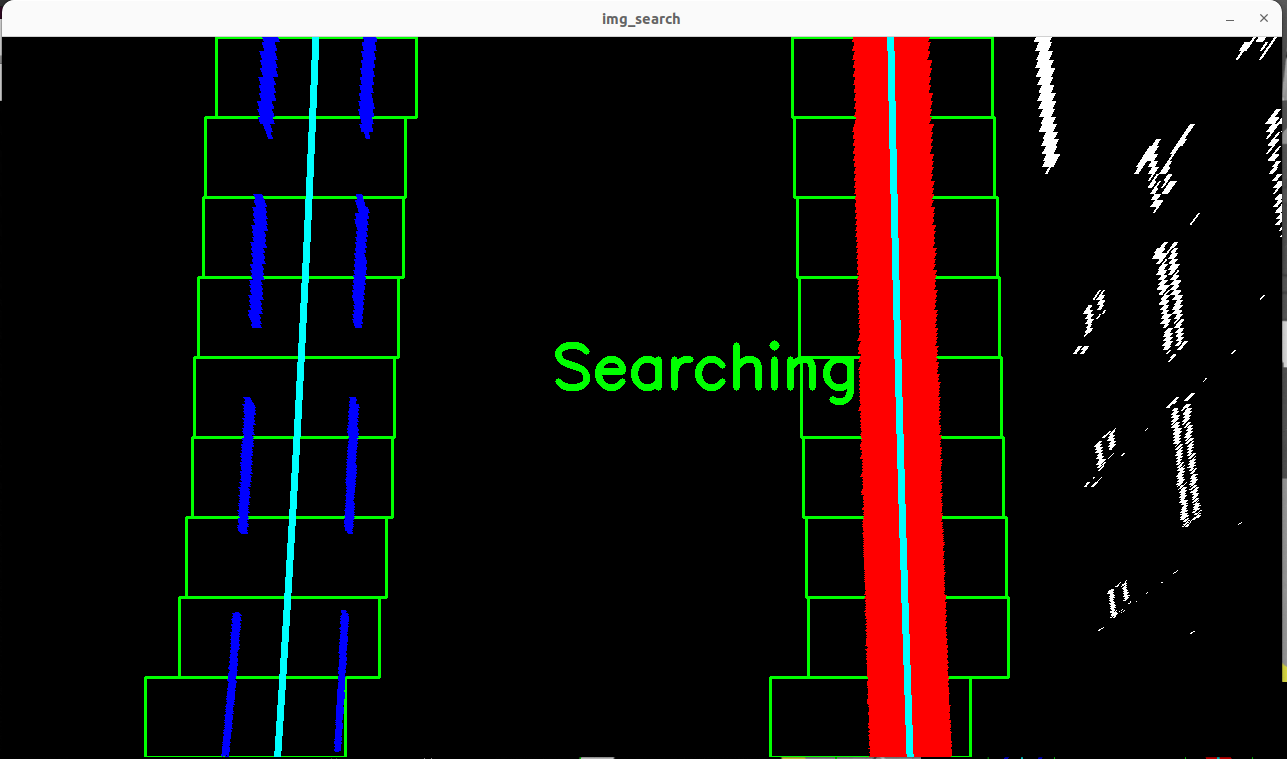
\includegraphics[width=0.6\linewidth]{images/3-lane/sliding.png}
    \caption{Nhận diện làn đường}
\end{figure}
\subsection{Tổng hợp}
Như vậy, sau khi có được thông tin của các đường thẳng (hoặc cong) fit với hai làn đường, từ đó ta sẽ sử dụng chúng để tính toán các thông số tiếp theo như là độ cong của mỗi làn, khoảng cách của xe với trung tâm của làn, ta cũng sẽ vẽ 1 đường nhầm thể hiện xu hướng rẽ trung bình của hai làn đường để biết rằng đường đang thẳng hay cong sang trái(phải).... Đồng thời ta sẽ để output chứa tất cả các hình ảnh của các bước trên với mục đích xe sẽ phải quản lí chặt chẽ các thông tin đó cũng như dễ dàng hơn cho việc debug sau này.\\
Ta thu được:
\begin{figure}[htbp]
    \centering
    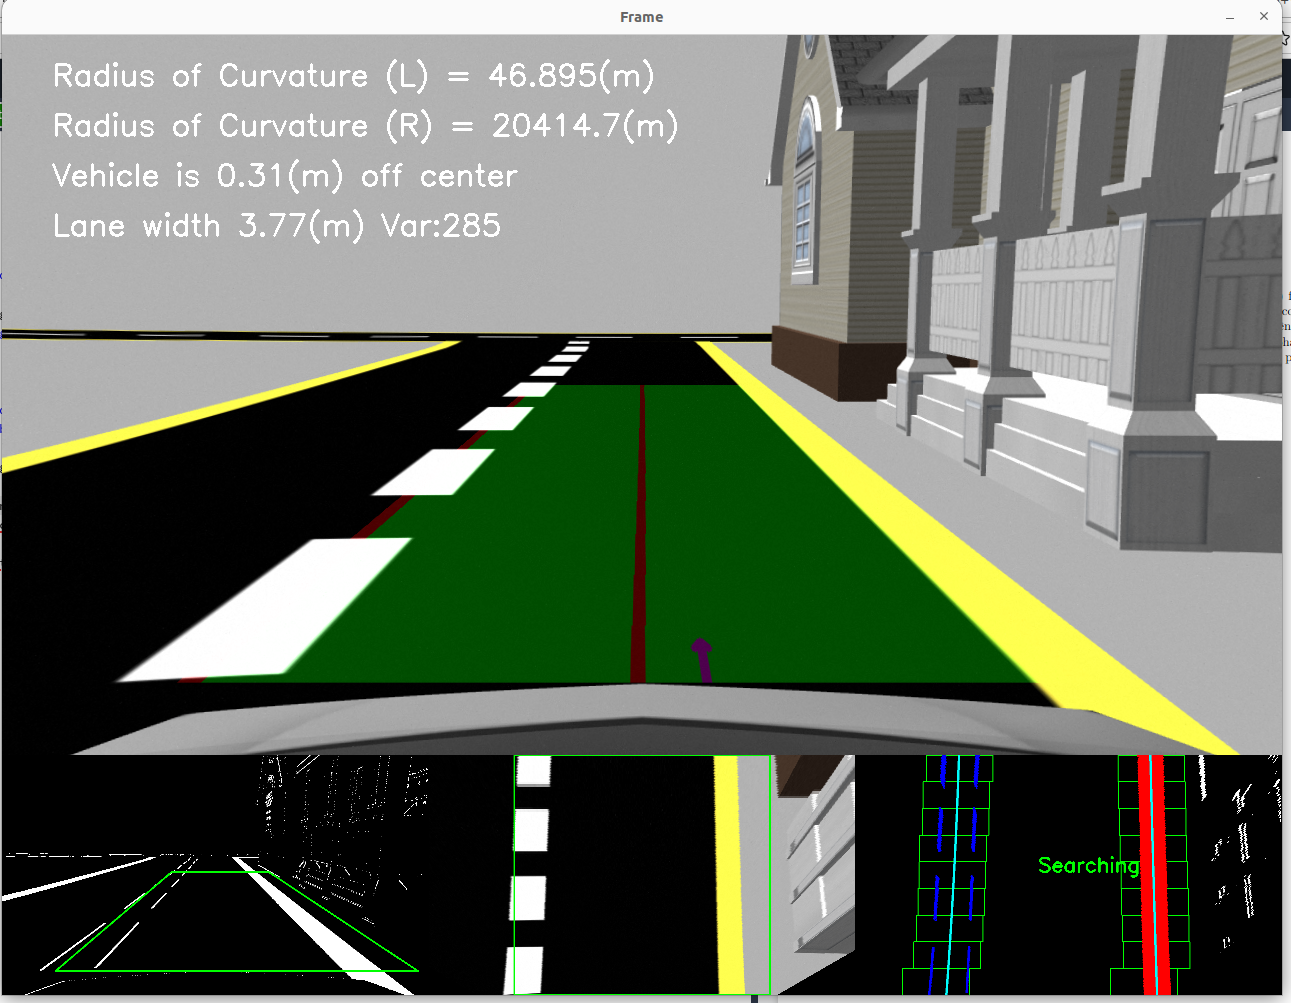
\includegraphics[width=0.8\linewidth]{images/3-lane/combine.png}
    \caption{Tổng hợp thông tin}
\end{figure}
\end{document}
